% B.Tech. Project: final presentation (Beamer)
% Build:  cd presentation && latexmk -pdf btp_final.tex
%   or:   pdflatex btp_final && pdflatex btp_final
% Figures are read directly from the repository result folders (see \graphicspath).
\documentclass[aspectratio=169,11pt,xcolor=table]{beamer}

\usetheme{Madrid}
\usecolortheme{default}
\usefonttheme{professionalfonts}

\usepackage[T1]{fontenc}
\usepackage{lmodern}
\usepackage{amsmath,amssymb}
\usepackage{booktabs}
\usepackage{multirow}
\usepackage{array}
\usepackage{tikz}
\usetikzlibrary{arrows.meta,positioning,shapes.geometric,fit,calc,backgrounds}
\usepackage{graphicx}

\graphicspath{%
  {../results/fhlm/figures/}%
  {../results/figures/}%
  {../results/}%
  {../paper/extended/figures/}%
  {../paper/figures/}%
  {../results/v2/}%
}

% ---------- colours ----------
\definecolor{iitblue}{RGB}{16,52,110}
\definecolor{accent}{RGB}{200,40,40}
\definecolor{good}{RGB}{20,120,60}
\definecolor{soft}{RGB}{235,240,248}
\setbeamercolor{structure}{fg=iitblue}
\setbeamercolor{palette primary}{bg=iitblue,fg=white}
\setbeamercolor{palette secondary}{bg=iitblue!85!black,fg=white}
\setbeamercolor{palette tertiary}{bg=iitblue!70!black,fg=white}
\setbeamercolor{frametitle}{bg=iitblue,fg=white}
\setbeamercolor{title}{bg=iitblue,fg=white}
\setbeamercolor{block title}{bg=iitblue,fg=white}
\setbeamercolor{block body}{bg=soft}
\setbeamercolor{block title alerted}{bg=accent,fg=white}
\setbeamercolor{block body alerted}{bg=accent!8}
\setbeamercolor{block title example}{bg=good,fg=white}
\setbeamercolor{block body example}{bg=good!8}
\setbeamertemplate{navigation symbols}{}
\setbeamertemplate{itemize items}[circle]
\setbeamertemplate{blocks}[rounded][shadow=false]
\setbeamerfont{frametitle}{size=\large,series=\bfseries}
\setbeamerfont{section in toc}{size=\small}
\makeatletter
\patchcmd{\beamer@sectionintoc}{\vskip1.5em}{\vskip0.6em}{}{}
\makeatother

\newcommand{\rstar}{r^{\ast}}
\newcommand{\hl}[1]{\textcolor{accent}{\textbf{#1}}}
\newcommand{\gd}[1]{\textcolor{good}{\textbf{#1}}}
\newcommand{\best}[1]{\textbf{\textcolor{good}{#1}}}

\AtBeginSection[]{%
  \begin{frame}[noframenumbering]{Outline}
    \tableofcontents[currentsection,hideallsubsections]
  \end{frame}
}

% ---------- title ----------
\title[Fronthaul Load Management in O-RAN]{Fronthaul Load Management for Open RAN}
\subtitle{IQ Compression by Matrix Decomposition and\\
Deadline-Feasible, Uncertainty-Aware Budget Allocation on a Shared 7-2x Link}
\author[M.~Yadav \& H.~Choudhary]{Mayank Yadav \and Harshvardhan Choudhary}
\institute[B.Tech. Project]{B.Tech. Project --- Final Evaluation}
\date{November 2026}

\begin{document}

% =====================================================================
\begin{frame}
  \titlepage
\end{frame}

\begin{frame}{Outline}
  \tableofcontents[hideallsubsections]
\end{frame}

% =====================================================================
\section{Introduction and Motivation}
% =====================================================================

\begin{frame}{What is the fronthaul and why is it loaded?}
  \small
  \begin{columns}[T]
    \begin{column}{0.55\textwidth}
      \begin{itemize}
        \item \textbf{Fronthaul} = link between the radio unit on the tower (\textbf{O-RU}) and the processing unit (\textbf{O-DU}).
        \item In the O-RAN \textbf{7-2x split} it carries frequency-domain \textbf{IQ samples} for every scheduled resource block (PRB).
        \item Rates are huge: raw 64-antenna cell $\approx$ \hl{15.4 Gbit/s}; 273 PRB $\times$ 4 layers at BFP-9: \hl{7.4 Gbit/s} peak.
        \item 7-2x load \emph{follows the scheduled traffic} $\Rightarrow$ operators \textbf{over-subscribe} one Ethernet link across many cells.
      \end{itemize}
    \end{column}
    \begin{column}{0.43\textwidth}
      \centering
      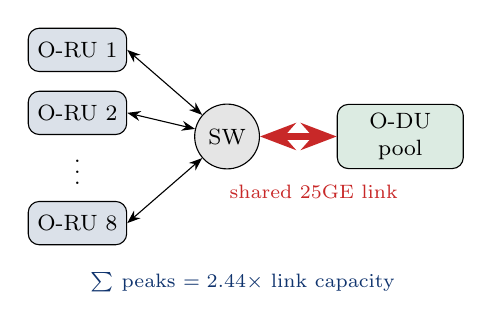
\begin{tikzpicture}[font=\footnotesize, >=Stealth,
        ru/.style={draw,fill=iitblue!15,rounded corners,minimum width=1.1cm,minimum height=0.55cm},
        box/.style={draw,fill=good!15,rounded corners,minimum width=1.6cm,minimum height=0.8cm}]
        \node[ru] (r1) at (0,2.4) {O-RU 1};
        \node[ru] (r2) at (0,1.6) {O-RU 2};
        \node at (0,0.95) {$\vdots$};
        \node[ru] (r8) at (0,0.2) {O-RU 8};
        \node[draw,fill=gray!20,circle,minimum size=0.8cm] (sw) at (1.9,1.3) {SW};
        \node[box,align=center] (du) at (4.1,1.3) {O-DU\\pool};
        \foreach \r in {r1,r2,r8} \draw[<->] (\r.east) -- (sw);
        \draw[<->,line width=2.2pt,accent] (sw) -- (du);
        \node[text=accent,font=\scriptsize] at (3.0,0.6) {shared 25GE link};
        \node[align=center,text=iitblue] at (2.1,-0.55) {\scriptsize $\sum$ peaks $=2.44\times$ link capacity};
      \end{tikzpicture}
    \end{column}
  \end{columns}
  \begin{alertblock}{Problem}
    When bursts of several cells coincide, the link cannot carry everything; low-latency cells tolerate only $\sim$2\,ms of waiting.
  \end{alertblock}
\end{frame}

\begin{frame}{Two levers for fronthaul load management}
  \centering
  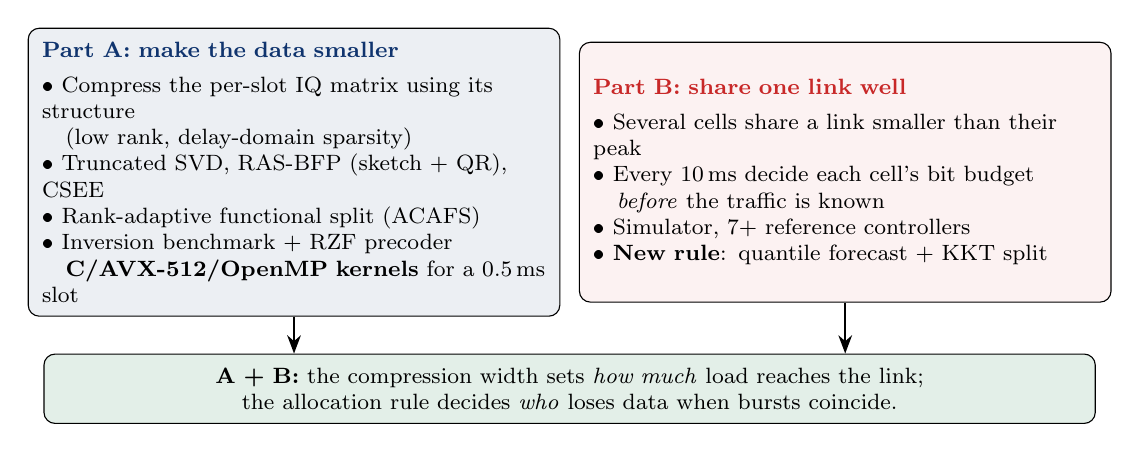
\begin{tikzpicture}[font=\footnotesize, >=Stealth,
     lever/.style={draw,rounded corners,align=left,text width=6.4cm,minimum height=3.3cm,inner sep=5pt}]
    \node[lever,fill=iitblue!8] (A) at (0,0) {%
      \textbf{\textcolor{iitblue}{Part A: make the data smaller}}\\[3pt]
      \textbullet\ Compress the per-slot IQ matrix using its structure\\
      \quad (low rank, delay-domain sparsity)\\
      \textbullet\ Truncated SVD, RAS-BFP (sketch + QR), CSEE\\
      \textbullet\ Rank-adaptive functional split (ACAFS)\\
      \textbullet\ Inversion benchmark + RZF precoder\\
      \quad \textbf{C/AVX-512/OpenMP kernels} for a 0.5\,ms slot};
    \node[lever,fill=accent!6] (B) at (7,0) {%
      \textbf{\textcolor{accent}{Part B: share one link well}}\\[3pt]
      \textbullet\ Several cells share a link smaller than their peak\\
      \textbullet\ Every 10\,ms decide each cell's bit budget\\
      \quad \emph{before} the traffic is known\\
      \textbullet\ Simulator, 7+ reference controllers\\
      \textbullet\ \textbf{New rule}: quantile forecast + KKT split};
    \node[draw,rounded corners,fill=good!12,text width=13cm,align=center,inner sep=5pt] (AB) at (3.5,-2.75) {%
      \textbf{A + B:} the compression width sets \emph{how much} load reaches the link;
      the allocation rule decides \emph{who} loses data when bursts coincide.};
    \draw[->,thick] (A.south) -- (A.south |- AB.north);
    \draw[->,thick] (B.south) -- (B.south |- AB.north);
  \end{tikzpicture}
\end{frame}

\begin{frame}{Objectives and contributions}
  \footnotesize
  \begin{enumerate}
    \item \textbf{Part A --- Compression and computation}
      \begin{itemize}
        \item Two structure-aware IQ encoders (\textbf{CSEE}, \textbf{RAS-BFP}) with error bounds, compared to O-RAN BFP and truncated SVD on 3GPP TDL-A channels.
        \item A rank-adaptive split controller (\textbf{ACAFS}).
        \item CPU benchmark of 9 matrix-inversion methods incl.\ learned inverters.
        \item Complex RZF precoding: RMT-guided warm-start inversion and a \textbf{fused C/AVX-512/OpenMP precoder kernel} (10--15$\times$ over numpy+LAPACK).
      \end{itemize}
    \item \textbf{Part B --- Shared-link budget allocation} (main work)
      \begin{itemize}
        \item Forecast the \textbf{deadline-feasible rate} $\rstar$ of each cell, not its volume.
        \item Closed-form \textbf{KKT (constrained newsvendor) rule} on a quantile forecast, with 4 propositions.
        \item Fair evaluation: 12 controllers, 2 traffic families, 20 test seeds, paired statistics.
      \end{itemize}
    \item \textbf{Extended study} --- MDP formulation, Markov-fluid theory of $\rstar$, a 3rd traffic family, 7 more controllers.
    \item \textbf{Part B2/B3} --- a modified Transformer forecaster (LCQT, Bayesian, decision-focused) and the \textbf{back-pressure newsvendor}, which beats predictive MaxWeight and CEM in 10/10 scenarios.
    \item \textbf{Outputs} --- NCC 2027 paper (6 pp.), 11-page extended manuscript, fully reproducible code (46 tests).
  \end{enumerate}
\end{frame}

% =====================================================================
\section{Part A: IQ Compression by Matrix Decomposition}
% =====================================================================

\begin{frame}{Part A system model}
  \begin{columns}[T]
    \begin{column}{0.52\textwidth}
      Received frequency-domain matrix after OFDM demodulation:
      \[
        Y = H \odot X + W \in \mathbb{C}^{M\times N}
      \]
      \begin{itemize}
        \item $M = 64$ antennas, $N = 1200$ subcarriers (100\,MHz class)
        \item 3GPP TR 38.901 \textbf{TDL-A} delay profile
        \item Exponential spatial correlation across antennas
      \end{itemize}
      Raw fronthaul rate (32-bit IQ, numerology 0):
      \[
        R_{\rm raw} = 2 M N_{\rm sc} N_{\rm sym}\, b\, R_{\rm slot} \approx 15.36~\text{Gbit/s/cell}
      \]
    \end{column}
    \begin{column}{0.45\textwidth}
      \begin{block}{Two structures to exploit}
        \begin{itemize}
          \item \textbf{Low rank}: correlated antennas $\Rightarrow$ numerical rank $r \ll \min(M,N)$
          \item \textbf{Delay sparsity}: few strong channel taps $\Rightarrow$ sparse after IFFT along subcarriers
        \end{itemize}
      \end{block}
      \begin{block}{Baseline: O-RAN BFP}
        Shared block exponent + $b$-bit mantissa per PRB. Only shortens numbers: $\approx 4\times$.
      \end{block}
    \end{column}
  \end{columns}
\end{frame}

\begin{frame}{Compression methods}
  \small
  \begin{columns}[T]
    \begin{column}{0.5\textwidth}
      \begin{block}{CSEE: delay-domain sparse encoder}
        $Y_d = \mathrm{IFFT}_N(Y)$,\ \ $S = \mathrm{TopK}(|Y_d|)$,\ \ $\hat Y = \mathrm{FFT}(Y_d|_S)$\\[2pt]
        Keep top-$K$ taps, per-antenna BFP.\\[2pt]
        \textbf{Thm 1:}\
          $\mathrm{NMSE} \le \dfrac{\sigma^2_{\rm tail}}{\sigma^2_Y} + \dfrac{\Delta^2}{12}\dfrac{K}{MN\sigma_Y^2}$
      \end{block}
    \end{column}
    \begin{column}{0.5\textwidth}
      \begin{block}{RAS-BFP: randomised sketch + QR}
        \begin{enumerate}
          \item SRHT sketch $Z = \Omega Y \in \mathbb{C}^{r\times N}$
          \item Thin QR: $Z^H = QR$;\ \ $L = YQ$
          \item Send $\mathrm{BFP}(L), \mathrm{BFP}(Q)$;\ \ $Y \approx L Q^H$
        \end{enumerate}
        \textbf{Thm 2:} $\|Y - LQ^H\|_F^2 \le (1+\varepsilon_r)\|Y - Y_r\|_F^2$ w.p.\ $\ge 1-\delta$\\
        \textbf{Thm 4:} $r^\star = \big\lfloor\sqrt{B_{\rm total}/(b(M+N))}\big\rceil$
      \end{block}
    \end{column}
  \end{columns}
  \vspace{0.1em}
  \centering
  \begin{tabular}{lll}
    \toprule
    Method & Complexity & Theory \\
    \midrule
    O-RAN BFP & $\mathcal{O}(MN)$ & empirical quantisation \\
    Truncated SVD & $\mathcal{O}(MN\min(M,N))$ & Eckart--Young \\
    \textbf{CSEE} & $\mathcal{O}(MN\log N)$ & Theorem 1 \\
    \textbf{RAS-BFP} & $\mathcal{O}(rMN)$ & Theorems 2--4 (Halko--Martinsson--Tropp) \\
    \bottomrule
  \end{tabular}
\end{frame}

\begin{frame}{ACAFS: rank-adaptive functional split}
  \begin{columns}[c]
    \begin{column}{0.48\textwidth}
      Per-UE rank fraction $r_k/M$ chooses the split:
      \begin{center}
        \begin{tabular}{cc}
          \toprule
          Rank fraction & Split \\
          \midrule
          $r/M < 0.15$ & 7.2x \\
          $0.15 \le r/M < 0.55$ & 7.1 \\
          $r/M \ge 0.55$ & 6 \\
          \bottomrule
        \end{tabular}
      \end{center}
      Uniform ranks: $\approx 33\,\%$ cut ($\tau_\ell = 0.15$, $\tau_h = 0.55$).\\
      Simulated: \textbf{0\,\%} below $\sim$15\,dB SNR, \textbf{55--75\,\%} above (rank collapse at high SNR).
    \end{column}
    \begin{column}{0.5\textwidth}
      \centering
      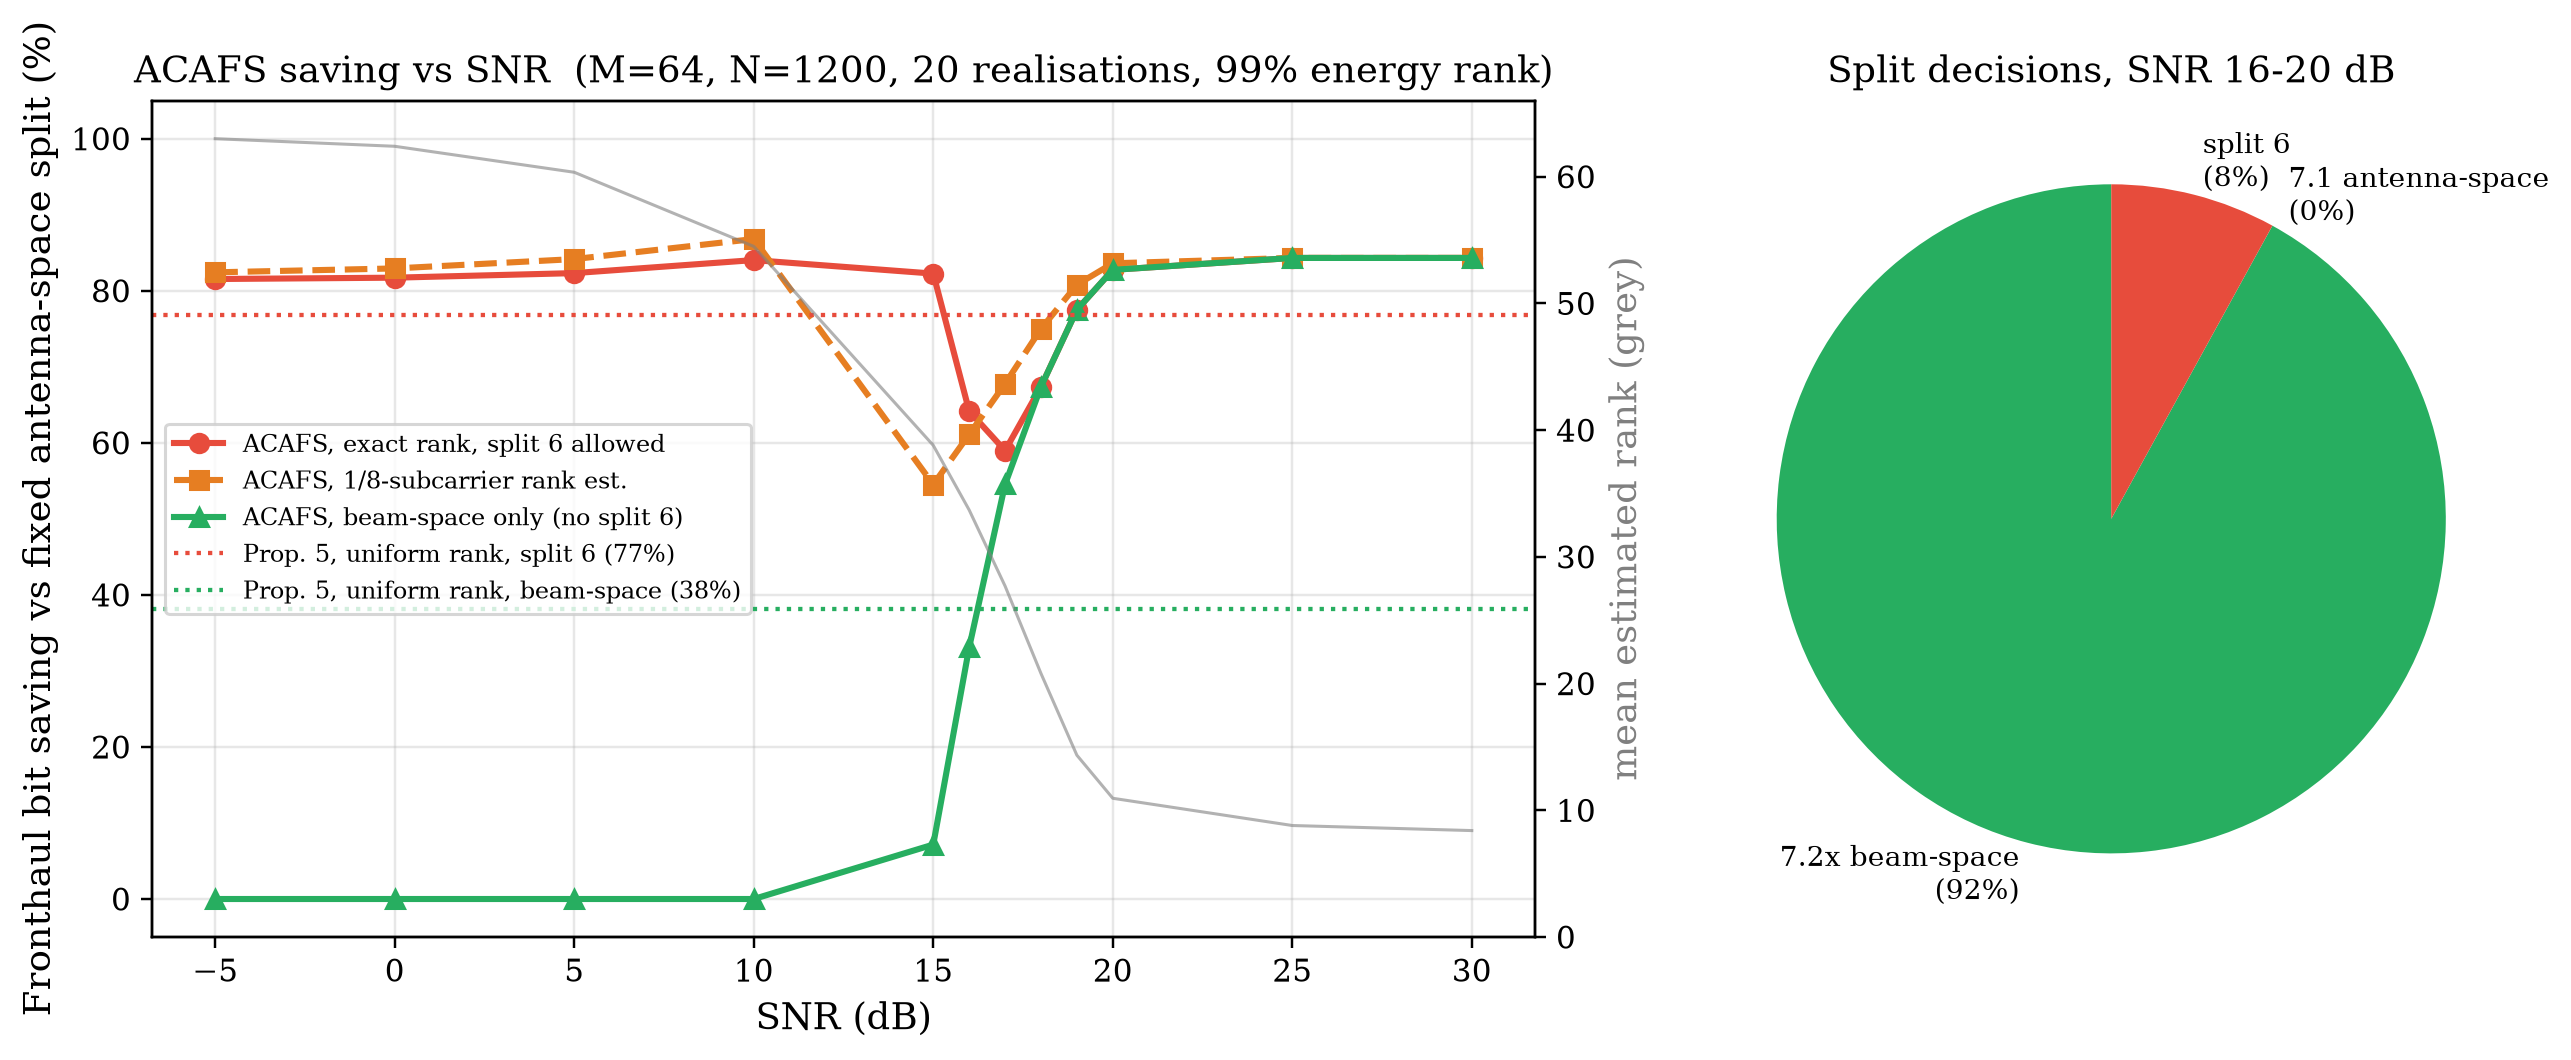
\includegraphics[width=\linewidth]{exp3_acafs.png}
    \end{column}
  \end{columns}
  \vspace{0.3em}
  \begin{block}{Theorem 5 (bandwidth cut vs.\ fixed Split 6)}
    \[
      \frac{\Delta \mathrm{BW}}{\mathrm{BW}_6} = 1 - \big(\mathrm{BW}_{7.2x}\,\tau_{\ell} + \mathrm{BW}_{7.1}(\tau_h-\tau_\ell) + \mathrm{BW}_6(1-\tau_h)\big)
    \]
  \end{block}
\end{frame}

\begin{frame}{Part A results: compression ratio vs.\ error}
  \begin{columns}[c]
    \begin{column}{0.5\textwidth}
      \centering
      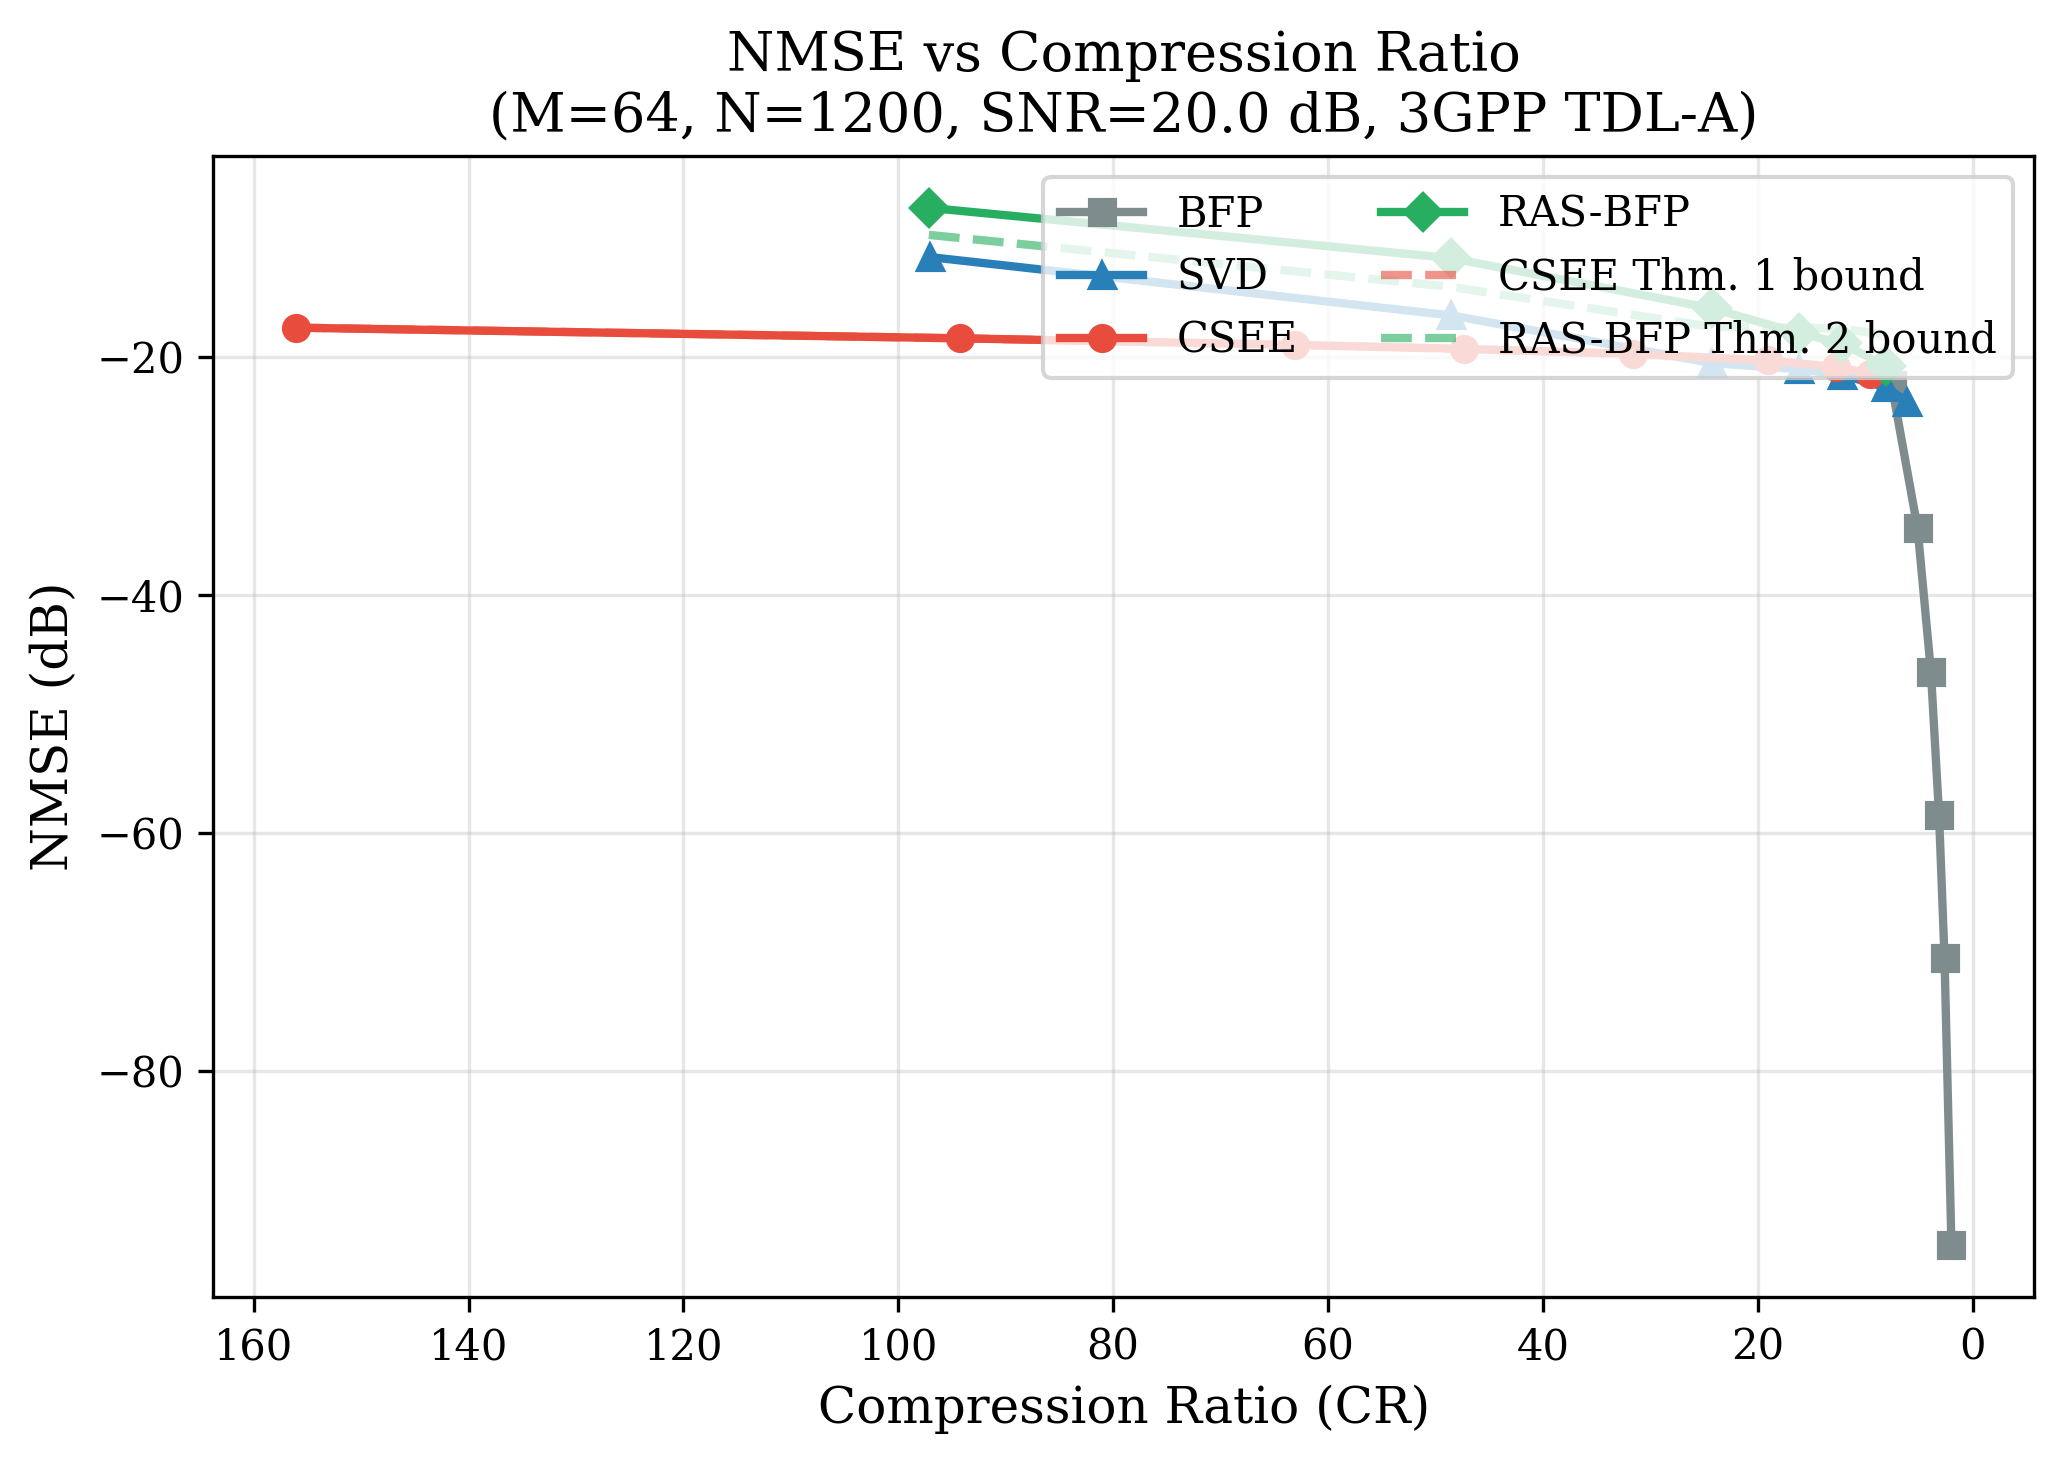
\includegraphics[width=\linewidth]{exp1_nmse_vs_cr.png}
    \end{column}
    \begin{column}{0.5\textwidth}
      \scriptsize
      $M=64$, $N=1200$, SNR 20\,dB, TDL-A\\[2pt]
      \begin{tabular}{lccc}
        \toprule
        Method & NMSE & CR & Encode \\
        \midrule
        BFP ($b=8$) & $-46$\,dB & $3.9\times$ & 3.1\,ms \\
        SVD ($r=12$) & $-21$\,dB & $16.2\times$ & 18--30\,ms \\
        \textbf{CSEE} ($K=300$) & $-21$\,dB & $12.7\times$ & \textbf{5.2\,ms} \\
        \textbf{RAS-BFP} ($r=12$) & $-18$\,dB & $16.2\times$ & \textbf{7.2\,ms} \\
        \bottomrule
      \end{tabular}
      \normalsize
      \vspace{0.5em}
      \begin{itemize}\small
        \item Structure-aware encoders reach \hl{13--16$\times$} at $\approx -20$\,dB vs.\ $\sim 4\times$ for BFP.
        \item RAS-BFP \textbf{3--4$\times$ faster} than SVD; CSEE \textbf{4--6$\times$ faster}.
        \item CSEE with $K=60$: $\sim$63$\times$ at $-19$\,dB (Pareto knee).
      \end{itemize}
    \end{column}
  \end{columns}
\end{frame}

\begin{frame}{Part A results: complexity and SNR robustness}
  \begin{columns}[T]
    \begin{column}{0.5\textwidth}
      \centering
      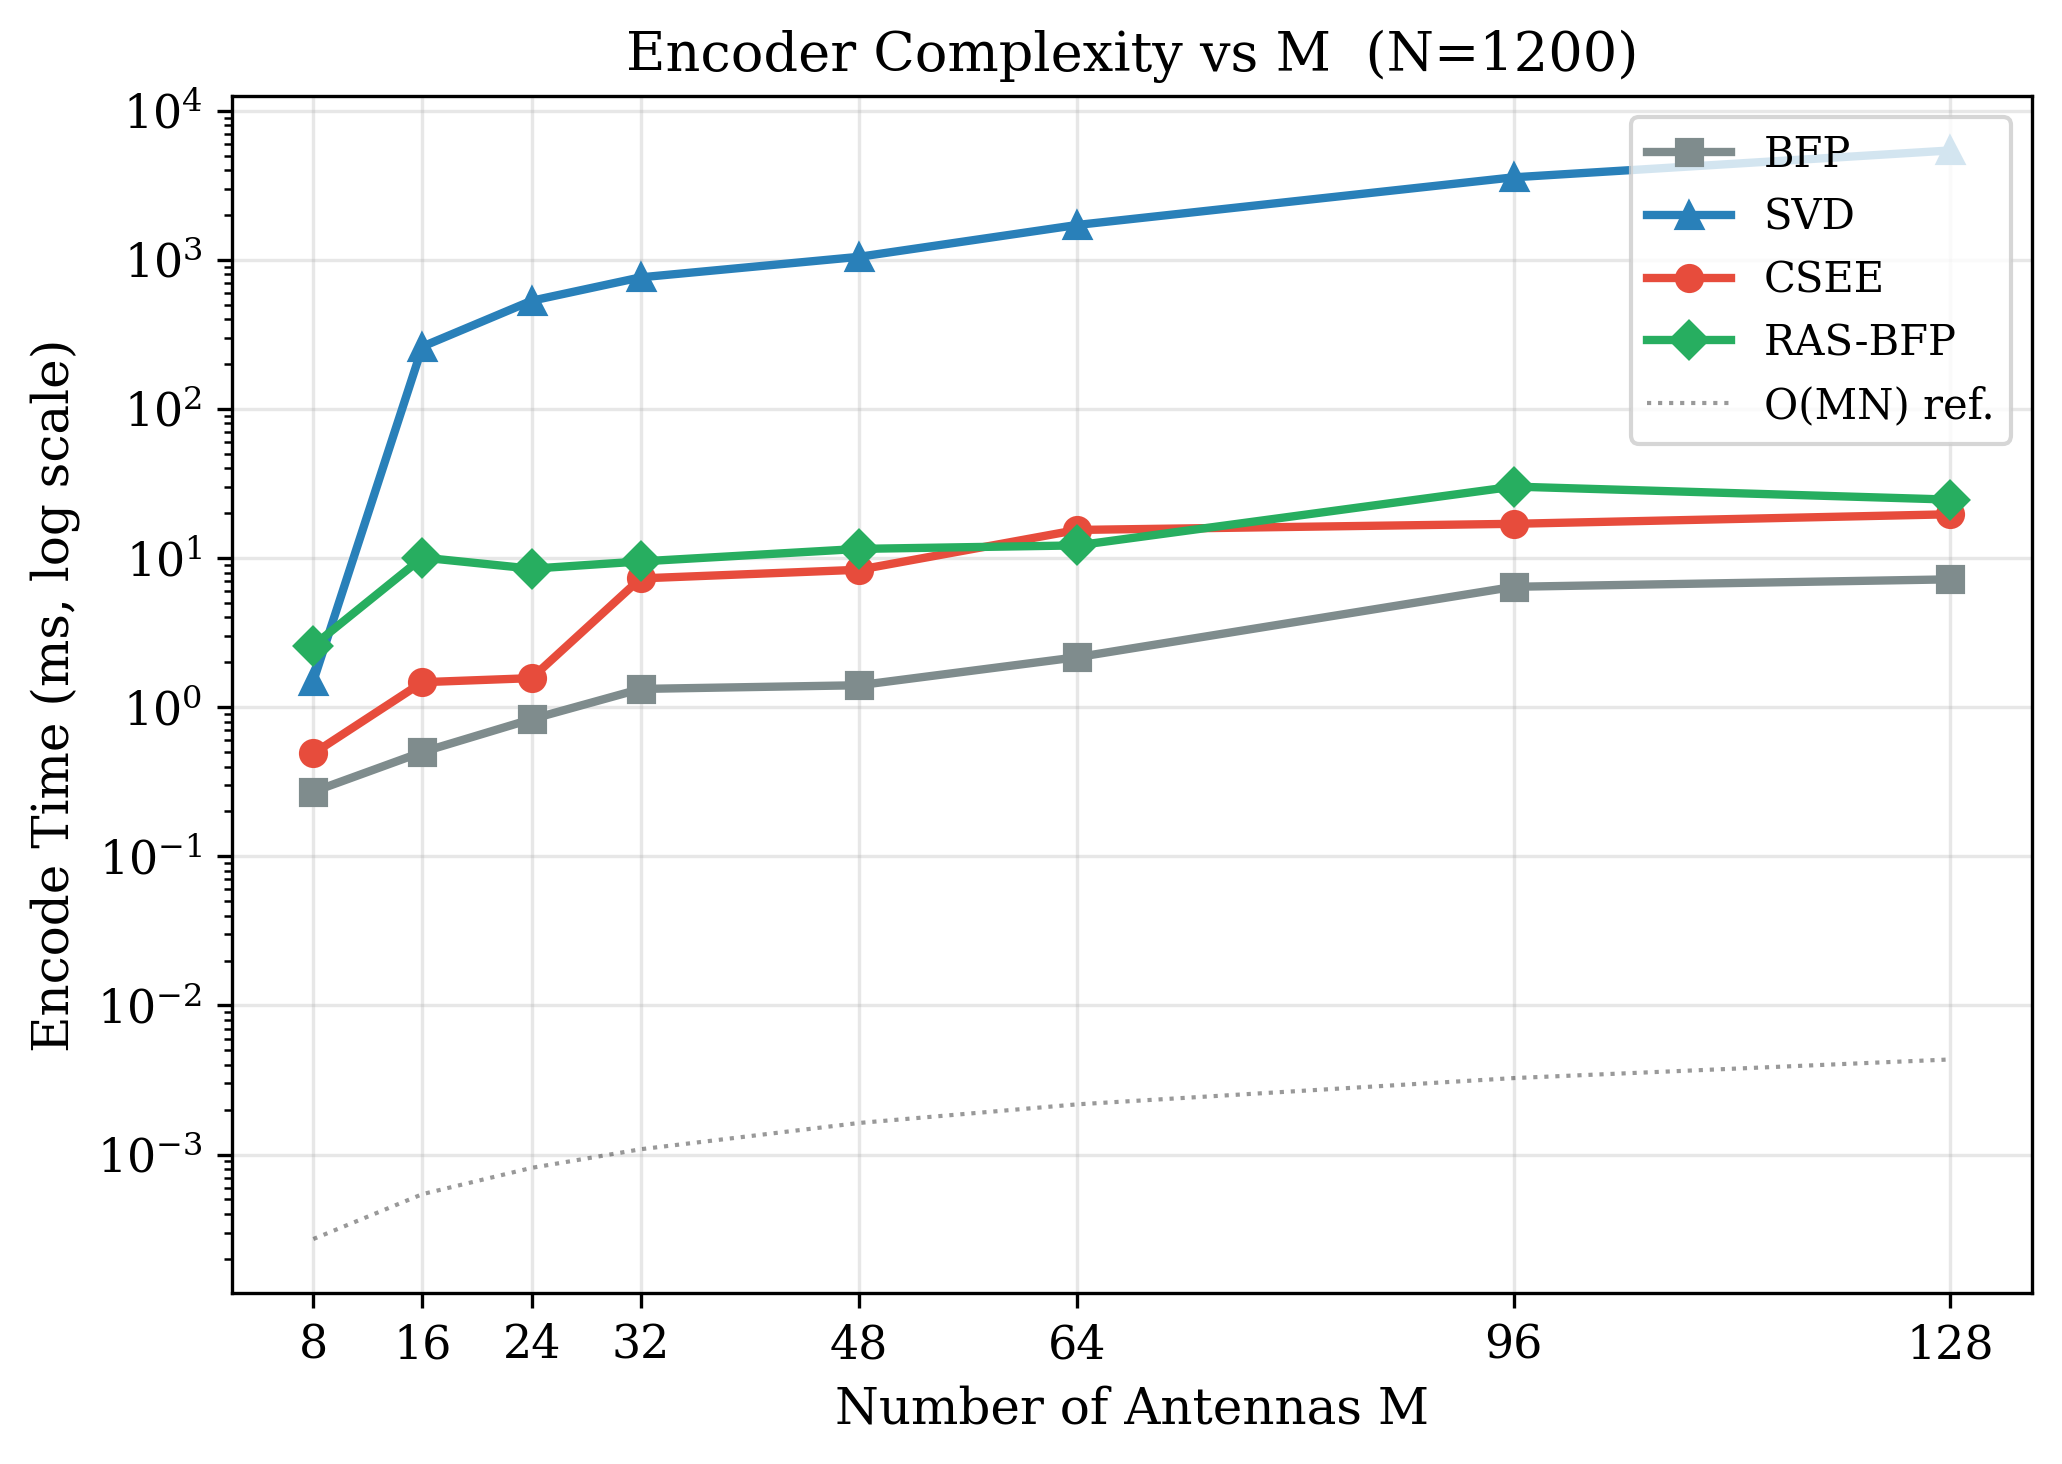
\includegraphics[width=\linewidth]{exp2_complexity.png}\\
      \small Encode time scaling: SVD grows fastest in $M$.
    \end{column}
    \begin{column}{0.5\textwidth}
      \centering
      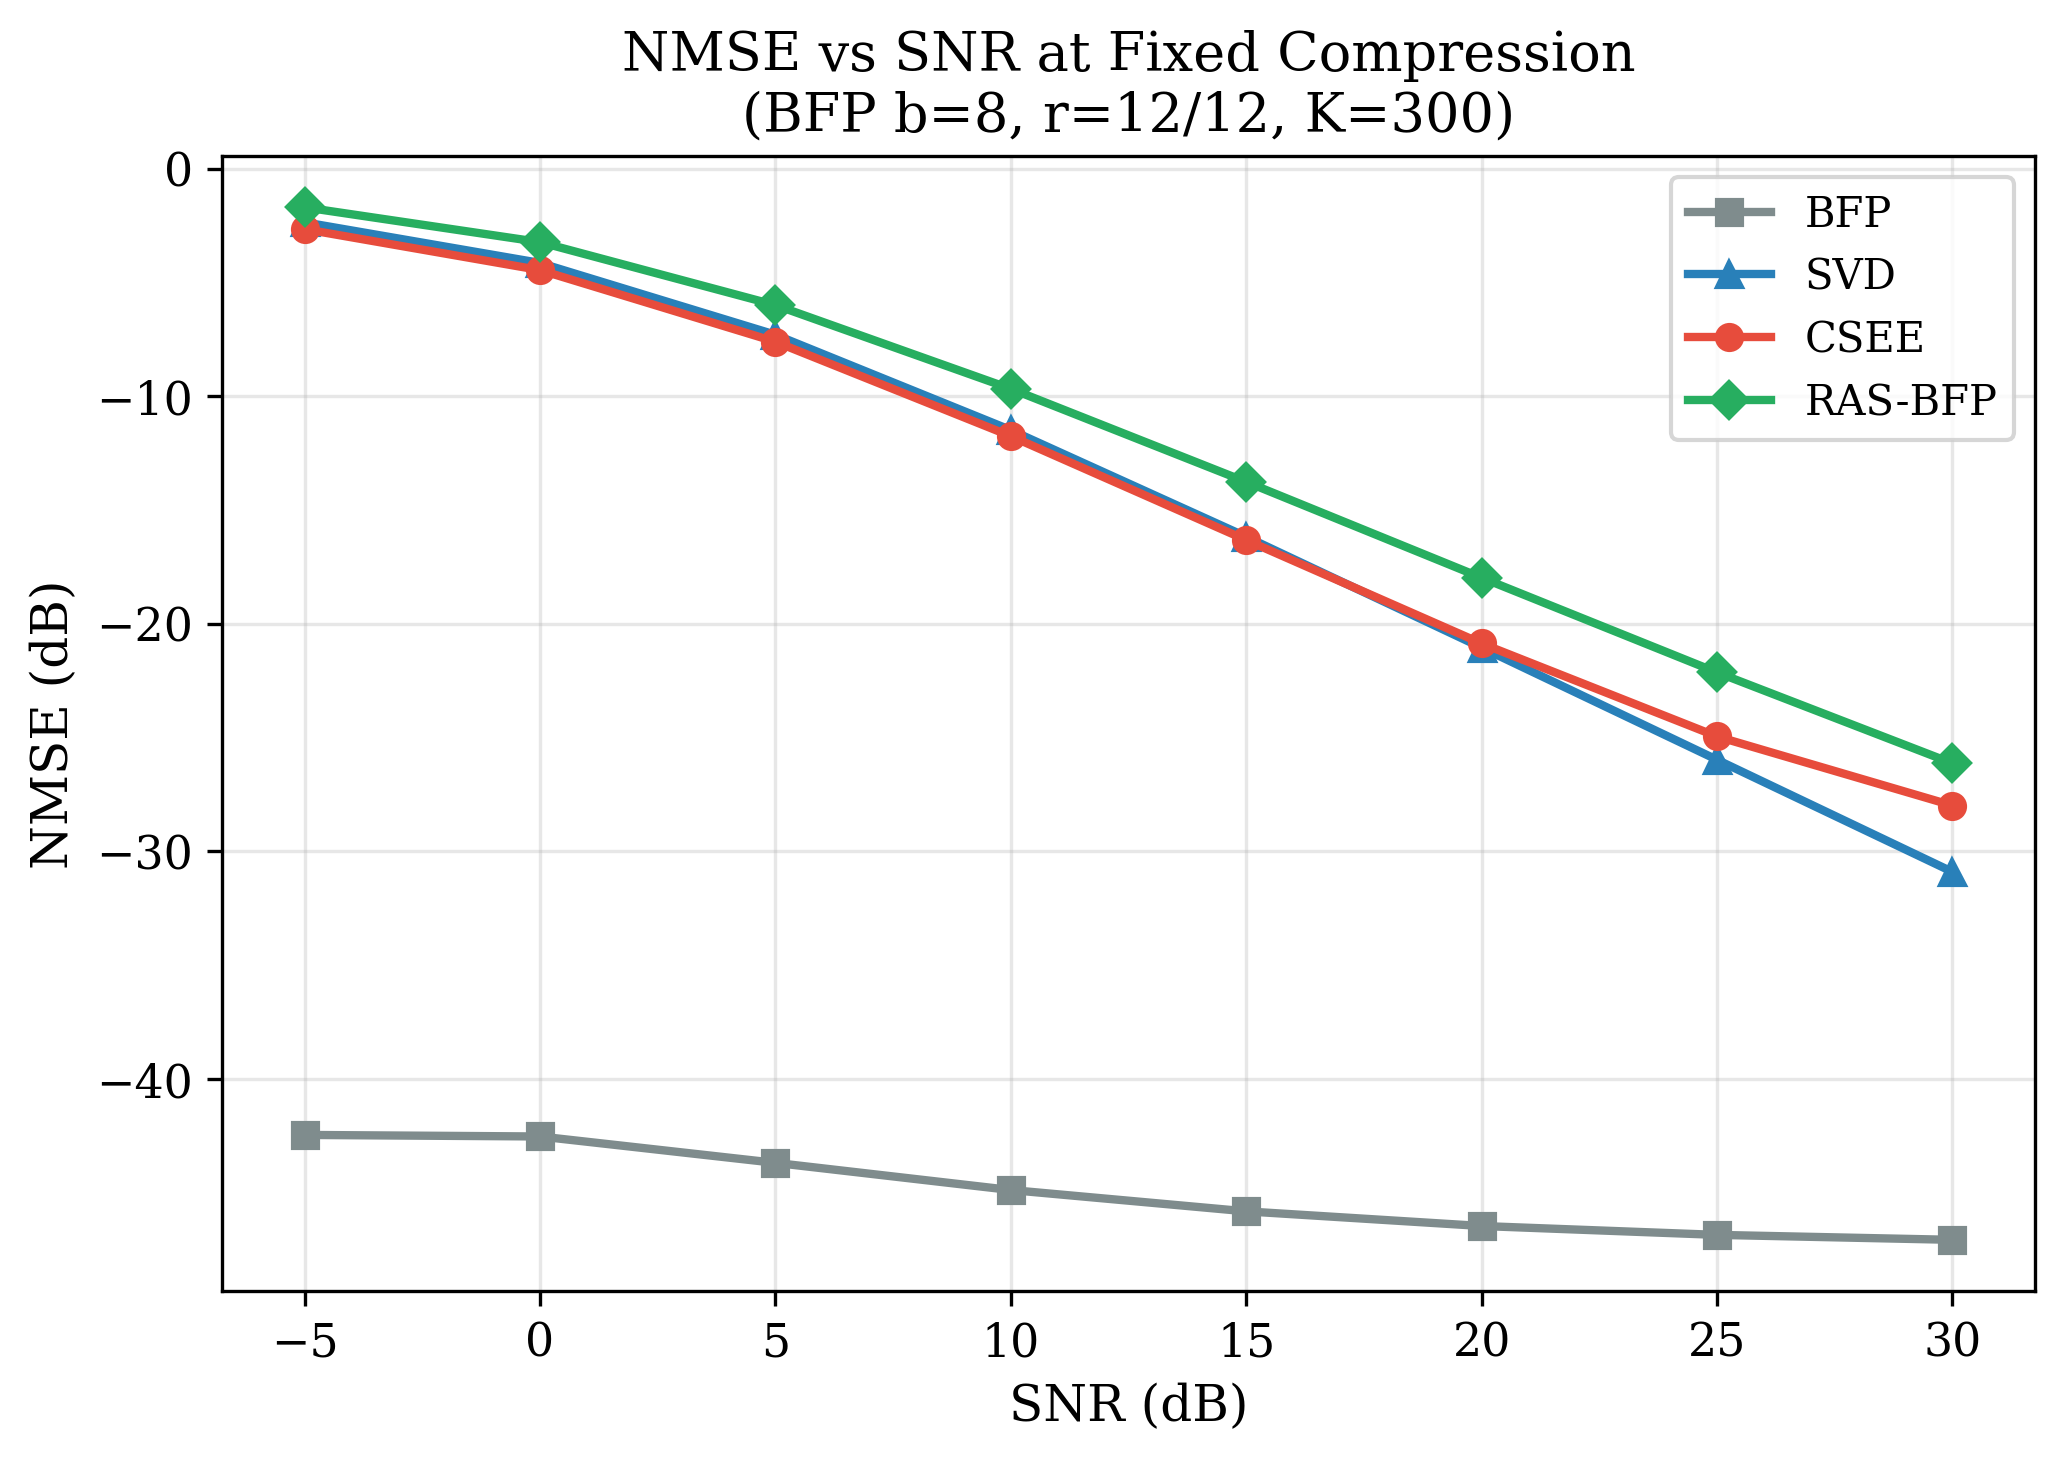
\includegraphics[width=\linewidth]{exp4_snr_sweep.png}\\
      \small NMSE stable across SNR $\in[-5, 30]$\,dB.
    \end{column}
  \end{columns}
\end{frame}

\begin{frame}{Matrix-inversion benchmark: why and how}
  \begin{columns}[T]
    \begin{column}{0.5\textwidth}
      \textbf{Why?} MMSE equalisation, ZF precoding, channel estimation and the encoders all need inverses/decompositions \emph{every slot} (0.5\,ms).
      \vspace{0.5em}

      \textbf{Dataset}
      \begin{itemize}
        \item $A = G/\sqrt{n} + 2I$, $G_{ij}\sim\mathcal N(0,1)$ (well conditioned)
        \item $n \in \{10, 100, 500\}$, 1000 samples each, float32
        \item 80\,\% train (neural models), timing on \textbf{200 held-out}
        \item Per matrix (batch 1), warm-up, CPU only
      \end{itemize}
    \end{column}
    \begin{column}{0.5\textwidth}
      \textbf{Methods}
      \begin{itemize}
        \item \textbf{Classical}: LAPACK getri, LU (scipy), QR, SVD, Gauss--Jordan, Newton--Schulz
        \item \textbf{InverseNet-MLP}: flatten $\to$ regress $A^{-1}$ directly (cannot scale: $>2\cdot10^9$ params at $n=500$)
        \item \textbf{InverseNet-NS}: unrolled Newton--Schulz, 8 steps, learned step coefficients
        \item \textbf{InverseNet-Ultra}: learned high-order iteration
      \end{itemize}
      Metrics: median / p95 time, relative error $\|X - A^{-1}\|_F / \|A^{-1}\|_F$.
    \end{column}
  \end{columns}
\end{frame}

\begin{frame}{Matrix-inversion benchmark: results}
  \begin{columns}[c]
    \begin{column}{0.52\textwidth}
      \centering
      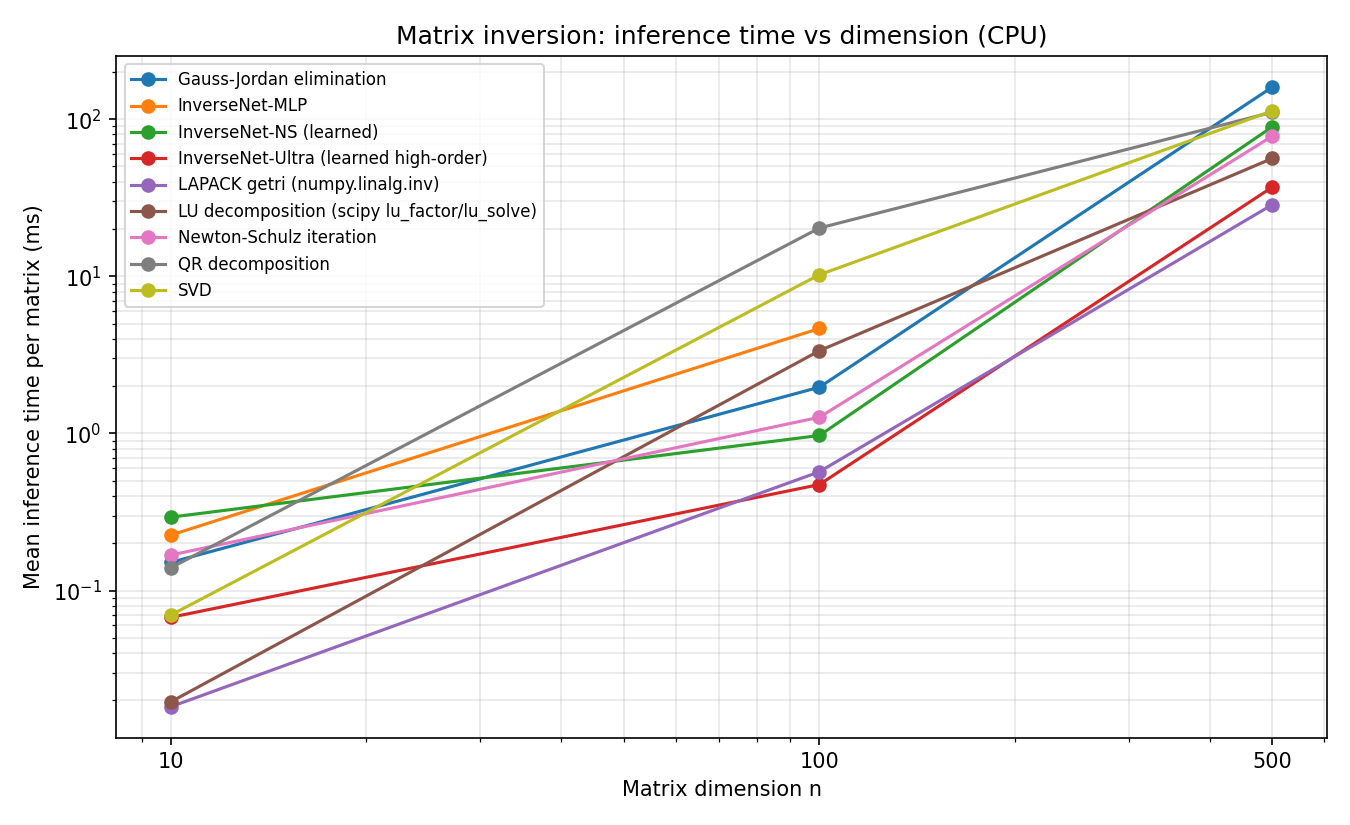
\includegraphics[width=\linewidth]{inference_time.png}
    \end{column}
    \begin{column}{0.48\textwidth}
      \scriptsize
      Median time [ms] and relative error (held-out)\\[2pt]
      \begin{tabular}{lrrr}
        \toprule
        Method & $n{=}100$ & $n{=}500$ & rel.\ err \\
        \midrule
        LAPACK getri & \best{0.17} & \best{18.0} & $5\!\cdot\!10^{-8}$ \\
        InverseNet-Ultra & 0.46 & 33.8 & $1\!\cdot\!10^{-6}$ \\
        InverseNet-NS & 0.95 & 92.1 & $4\!\cdot\!10^{-4}$ \\
        Newton--Schulz & 1.02 & 70.3 & $2\!\cdot\!10^{-7}$ \\
        SVD & 2.76 & 106.9 & $1\!\cdot\!10^{-7}$ \\
        LU (scipy) & 2.87 & 56.3 & $1\!\cdot\!10^{-7}$ \\
        QR & 3.94 & 102.2 & $3\!\cdot\!10^{-7}$ \\
        InverseNet-MLP & 4.58 & n/a & \hl{0.52} \\
        \bottomrule
      \end{tabular}
    \end{column}
  \end{columns}
\end{frame}

\begin{frame}{Part A: lessons}
  \begin{itemize}
    \item \textbf{LU via LAPACK} is the method to beat: fastest exact method at every size.
    \item \textbf{Slot budget}: $n \approx 100$ fits a 0.5\,ms slot on one CPU core; $n \approx 500$ (18\,ms) does not $\Rightarrow$ invert per coherence interval, track incrementally, or offload.
    \item \textbf{Direct neural inverse fails} ($\sim$50\,\% error): the matrix $\to$ inverse map is non-smooth with $n^2$ outputs.
    \item \textbf{Learned iteration works} ($10^{-6}$ error): keep the Newton--Schulz structure, learn only coefficients; fixed, predictable cost of batched matmuls (GPU/NPU friendly).
    \item \textbf{Predictability matters}: LAPACK p95 can be $5$--$10\times$ the median under thread contention; fixed-step methods are flat.
  \end{itemize}
  \begin{exampleblock}{Theme carried into Part B}
    Keep the mathematical structure and \textbf{learn only what is uncertain}.
  \end{exampleblock}
\end{frame}

% =====================================================================
\section{Part A2: Precoding Inversion and Kernel Programming}
% =====================================================================

\begin{frame}{From real benchmarks to the real workload: RZF precoding}
  \footnotesize
  \begin{columns}[T]
    \begin{column}{0.52\textwidth}
      \textbf{Gaps in the first benchmark}
      \begin{itemize}\footnotesize
        \item Real, i.i.d., well-conditioned $A = G/\sqrt n + 2I$; precoding needs \textbf{complex Hermitian} Grams of \textbf{correlated, near-far} channels.
        \item ``InverseNet-Ultra beats LAPACK'' holds only for the mean, not the median.
        \item The slot-to-slot warm start proposed in \texttt{REPORT.md} was never measured.
        \item No link from inversion to the fronthaul.
      \end{itemize}
      \textbf{New study} (\texttt{cmatinv/}, \texttt{experiments\_v2/})
      \begin{itemize}\footnotesize
        \item 38.901 UMa near-far, TDL-A, spatial correlation, Rician LoS, Jakes aging
        \item $M{=}64$, $K{=}16$, 273 PRBs, 0.5\,ms slots, 3.5\,GHz
      \end{itemize}
    \end{column}
    \begin{column}{0.46\textwidth}
      \begin{block}{Per-PRB RZF precoder (every slot)}
        \[
          G = HH^H + \alpha I \in \mathbb{C}^{K\times K}
        \]
        \[
          W = H^H G^{-1} \in \mathbb{C}^{M\times K}
        \]
        $\times\,273$ PRBs inside a \textbf{0.5\,ms} slot.
      \end{block}
      \begin{alertblock}{Question}
        Can the whole precoder (Gram + inverse + $W$) fit in a slot on a CPU, and can a warm-started iteration make the inverse cheaper?
      \end{alertblock}
    \end{column}
  \end{columns}
\end{frame}

\begin{frame}{RMT-WS: random-matrix-guided warm-start inversion}
  \footnotesize
  \begin{columns}[T]
    \begin{column}{0.55\textwidth}
      \begin{enumerate}
        \item \textbf{Equilibrate} $\hat G = D^{-1/2} G D^{-1/2}$ (removes the near-far spread).
        \item \textbf{Eigensolve-free spectral interval} (Marchenko--Pastur + moment match): $v = \|\hat G\|_F^2/K - 1$,\
          $[a,b] = 1 + v/\bar s \mp 2\sqrt v$ (cost $K^2$).
        \item \textbf{Cold start}: Chebyshev polynomial on $[a,b]$, then Newton--Schulz $X \leftarrow X(2I - \hat G X)$.
        \item \textbf{Tracking}: next slot starts from the previous inverse.
        \item \textbf{Residual certificate} $\|(I - \hat G X)z\|/\|z\|$ (2 probes, $4K^2$ MACs) picks the number of Newton steps, or falls back to a cold start when $r > 0.3$.
      \end{enumerate}
    \end{column}
    \begin{column}{0.43\textwidth}
      \begin{block}{Doppler-to-warm-start law}
        \[
          r_0 \approx c\cdot 2\sqrt{\tfrac{K}{M-K}}\sqrt{1-\rho},\quad 1-\rho \approx (\pi f_D T)^2
        \]
        $r_0$ grows \textbf{linearly with speed} (measured slope 1.00). Warm start valid up to $\approx$ \textbf{39\,km/h} ($M{=}64$, $K{=}16$), 60\,km/h ($K{=}8$), 23\,km/h ($K{=}32$).
      \end{block}
      \begin{block}{Certificate safety}
        Tail bound $\Pr(\hat r^2 \le (1-d)r^2) \le e^{-pd^2 s/2}$; audit of 480 cases: \textbf{0} accepted-but-non-contractive at $\hat r \le 0.3$.
      \end{block}
    \end{column}
  \end{columns}
\end{frame}

\begin{frame}{Inversion results: operation count and tracking}
  \footnotesize
  \begin{columns}[T]
    \begin{column}{0.48\textwidth}
      \textbf{GEMMs for $\le 1\,\%$ sum-rate loss} (cold start)\\[2pt]
      \begin{tabular}{lccc}
        \toprule
        Method & 64/16 & 128/16 & 64/32 \\
        \midrule
        Neumann (Wu/Prabhu) & $>8$ & $>8$ & $>8$ \\
        Joint Newton-Neumann & $>10$ & $>10$ & $>10$ \\
        Newton--Schulz, classic & $>10$ & $>10$ & $>10$ \\
        \textbf{Cheb-MP + NS (ours)} & \textbf{6} & 5 & \textbf{9} \\
        Gauss--Seidel & \textbf{6} & \textbf{4} & $>12$ \\
        Block CG & 7 & 5 & 12 \\
        \bottomrule
      \end{tabular}\\[3pt]
      Beats Neumann-type schemes; \hl{ties or loses} to Gauss--Seidel/CG at $K/M \le 0.25$. An exact Cholesky/LU inverse costs $\approx 1$ GEMM.
    \end{column}
    \begin{column}{0.5\textwidth}
      \textbf{Tracking}, $K{=}16$, $M{=}64$, 95\,\% CI over 16 drops\\[2pt]
      \begin{tabular}{lcc}
        \toprule
        Speed & Cold start (6 GEMM) & \textbf{RMT-WS} \\
        \midrule
        3\,km/h & 0.41\,\% & \best{0.011\,\% @ 2.25} \\
        30\,km/h & 0.41\,\% & 0.62\,\% @ 5.4 \\
        120\,km/h & 0.39\,\% & 0.39\,\% @ 6.25 \\
        \bottomrule
      \end{tabular}\\[3pt]
      \begin{itemize}
        \item 3\,km/h: \textbf{2.7$\times$ fewer GEMMs}, 30$\times$ lower loss.
        \item 30\,km/h: a wash; 120\,km/h: becomes a cold start (never diverges, unlike fixed warm starts).
        \item Low precision (8-bit mantissa, wide accumulate): 0.15\,\% vs 0.88\,\% for direct Gauss--Jordan.
      \end{itemize}
    \end{column}
  \end{columns}
\end{frame}

\begin{frame}{Where should precoding run? Fronthaul impact}
  \small
  \centering
  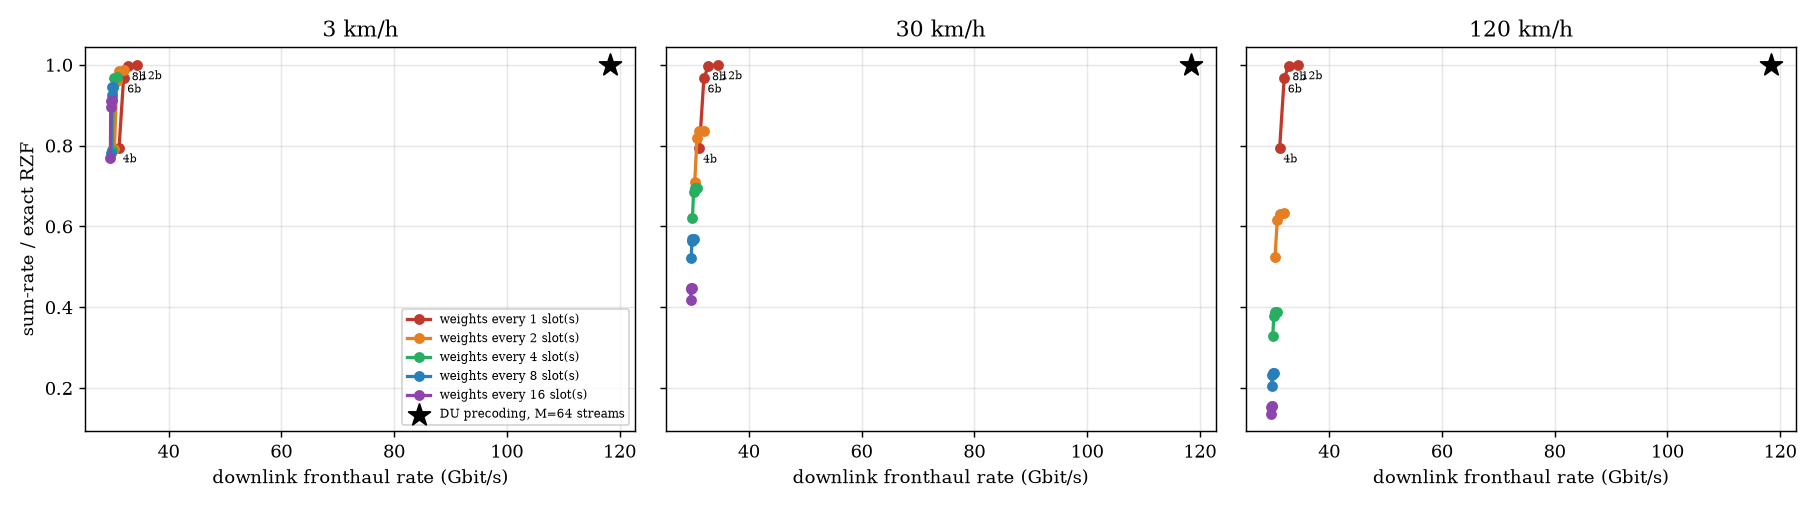
\includegraphics[width=0.92\linewidth]{exp10_fronthaul.png}\\[2pt]
  \footnotesize
  \begin{tabular}{lcc}
    \toprule
    Architecture (100\,MHz, $M{=}64$, $K{=}16$, BFP-9 IQ) & Fronthaul & Sum-rate vs exact RZF \\
    \midrule
    DU precodes, sends $M = 64$ streams & 118.4\,Gbit/s & 100\,\% \\
    RU precodes, $K = 16$ layers + 8-bit weights every slot & \textbf{32.8\,Gbit/s ($-72$\,\%)} & 99.7\,\% \\
    RU precodes, $K = 16$ layers + 6-bit weights every slot & 32.0\,Gbit/s ($-73$\,\%) & 96.7\,\% \\
    \bottomrule
  \end{tabular}\\[3pt]
  \raggedright
  At mobility the weights must be refreshed \textbf{every slot} (every 4 slots: 70\,\% rate at 30\,km/h) --- exactly the workload a fast per-slot precoder kernel serves. Caveat: saving assumes 3-PRB weight groups; per-subcarrier weights would exceed the DU-side rate.
\end{frame}

\begin{frame}[fragile]{Kernel programming: a fused RZF precoder in C}
  \scriptsize
  \begin{columns}[T]
    \begin{column}{0.5\textwidth}
      \textbf{\texttt{kernels/cmat\_kernels.c}} (batched complex64, Python binding \texttt{cmatinv/fastkernels.py})
      \begin{itemize}
        \item \textbf{One pass per PRB}: load $H$ once $\to$ Gram (lower triangle) $\to$ inverse $\to$ $W^T$ + power scaling; all stack/L1-resident, no DRAM intermediates.
        \item \textbf{Split re/im planes} (SoA) so complex arithmetic vectorises.
        \item \textbf{OpenMP} \texttt{parallel for} across the 273 PRBs; \texttt{omp simd} inner loops.
        \item \textbf{Gauss--Jordan sweep inverse}: $K$ rank-1 updates, contiguous fully-vectorised rows, no sqrt/divide chains; no pivoting needed since $G \succ 0$ (Cholesky kept behind \texttt{-DUSE\_CHOL}).
        \item \textbf{Register-blocked} $W = H^H X$; \textbf{AVX-512} codegen; \texttt{rdtsc} profiling.
        \item \textbf{Fused Newton step} returns the \emph{exact} residual $\|I - GX\|_F/\sqrt K$ for free.
      \end{itemize}
    \end{column}
    \begin{column}{0.48\textwidth}
      \textbf{Inner loop of the sweep inverse}
\begin{verbatim}
for (int i = 0; i < K; i++) {
  if (i == k) continue;
  float fr = ckr[i]*piv, fi = cki[i]*piv;
  float *ar = xr + i*K, *ai = xi + i*K;
  #pragma omp simd
  for (int j = 0; j < K; j++) {
    ar[j] -= fr*rkr[j] - fi*rki[j];
    ai[j] -= fr*rki[j] + fi*rkr[j];
  }
  ar[k] = -fr; ai[k] = -fi;
}
\end{verbatim}
      \textbf{Build} (\texttt{kernels/build.sh})
\begin{verbatim}
gcc -O3 -march=native -fopenmp -ffast-math
    -mprefer-vector-width=512 -shared -fPIC
\end{verbatim}
    \end{column}
  \end{columns}
\end{frame}

\begin{frame}{Kernel optimisation log (profiling-driven)}
  \small
  \begin{columns}[T]
    \begin{column}{0.52\textwidth}
      Per-stage cycles per PRB ($K{=}16$, $M{=}64$, 1 thread):
      \begin{enumerate}
        \item \textbf{Fusion + Hermitian symmetry}: Gram on lower triangle only.
        \item \textbf{Register-blocked axpy} $W = H^H X$, output $W^T[S,K,M]$: 0.81 $\to$ \textbf{0.42\,ms}/slot.
        \item \textbf{GJ sweep instead of Cholesky}: inverse 6.4k $\to$ \textbf{2.9k} cycles ($K{=}16$); 21k $\to$ 11k ($K{=}32$).
        \item \textbf{AVX-512} (\texttt{-mprefer-vector-width=512}; gcc uses 256-bit by default): 1.3--1.5$\times$ single-thread, 2$\times$ on 4 threads.
        \item 4-column blocked Gram: \hl{slower, reverted}.
      \end{enumerate}
    \end{column}
    \begin{column}{0.46\textwidth}
      \begin{block}{Where the cycles go after tuning}
        \begin{itemize}
          \item \texttt{form\_w} ($K\!\times\!K$ by $K\!\times\!M$): \textbf{44--58\,\%}, $\approx$30 flops/cycle ($\sim$half AVX-512 peak)
          \item Gram: 20--24\,\%, $\approx$28 flops/cycle
          \item Inverse: the rest
        \end{itemize}
      \end{block}
      \begin{block}{Accuracy}
        float32 kernel vs float64 exact: element error $\approx 3\cdot10^{-7}$, sum-rate loss $< 10^{-5}\,\%$ (incl.\ ill-conditioned, $K{=}32$, 30\,dB).
      \end{block}
    \end{column}
  \end{columns}
\end{frame}

\begin{frame}{Kernel results: whole precoder per slot (273 PRBs)}
  \begin{columns}[c]
    \begin{column}{0.52\textwidth}
      \centering
      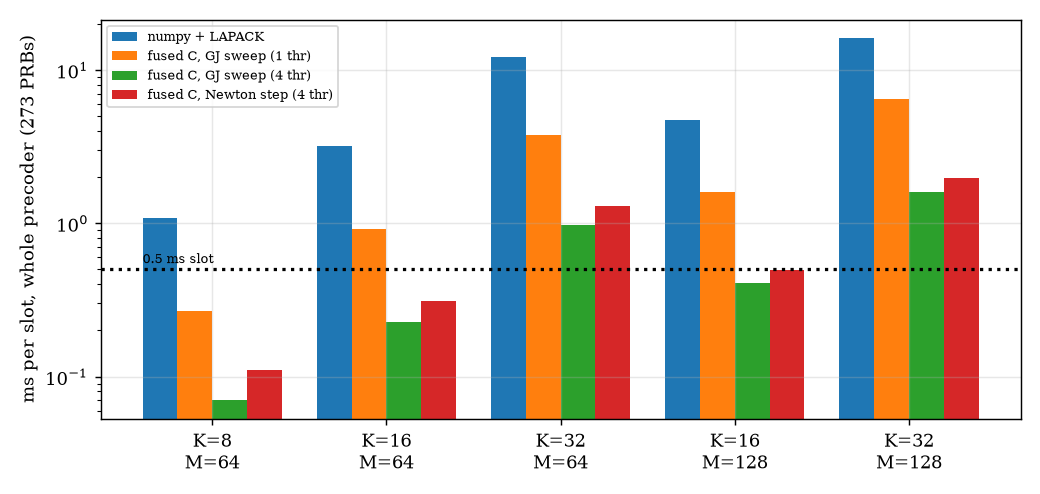
\includegraphics[width=\linewidth]{exp17_pipeline_kernel.png}
    \end{column}
    \begin{column}{0.46\textwidth}
      \scriptsize
      4-core AVX-512 Xeon, complex64, median of 40 runs\\[2pt]
      \setlength{\tabcolsep}{3pt}
      \begin{tabular}{lcccc}
        \toprule
        $K$,$M$ & numpy+LAPACK & C 1\,thr & C 4\,thr & gain \\
        \midrule
        8, 64 & 1.08\,ms & 0.27 & \best{0.070} & 15$\times$ \\
        16, 64 & 3.21\,ms & 0.92 & \best{0.226} & 14$\times$ \\
        32, 64 & 12.2\,ms & 3.75 & 0.97 & 12.5$\times$ \\
        16, 128 & 4.71\,ms & 1.61 & \best{0.41} & 11.6$\times$ \\
        32, 128 & 16.3\,ms & 6.43 & 1.60 & 10$\times$ \\
        \bottomrule
      \end{tabular}
      \normalsize
      \begin{itemize}\small
        \item $K = 8, 16$ ($M{=}64$) and $K{=}16$, $M{=}128$ now \textbf{fit a 0.5\,ms slot} for the \emph{entire} precoder (none did before).
        \item Near-linear thread scaling: 0.92 $\to$ 0.45 $\to$ 0.23\,ms (1/2/4 threads).
        \item The Newton-step path (0.31\,ms) is slower than the exact GJ sweep (0.23\,ms) inside the fused pipeline.
      \end{itemize}
    \end{column}
  \end{columns}
\end{frame}

\begin{frame}{Kernel programming: honest corrections and negative results}
  \small
  \begin{columns}[T]
    \begin{column}{0.5\textwidth}
      \centering
      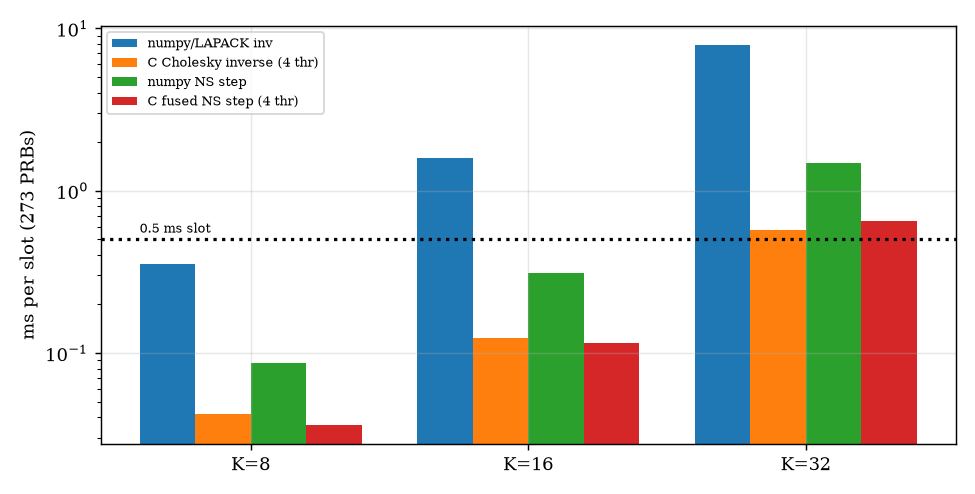
\includegraphics[width=\linewidth]{exp15_kernel_bench.png}\\
      \footnotesize Inverse only: tuned C Cholesky vs fused NS step (4 threads)
      \begin{exampleblock}{Verdict}
        \footnotesize Solid kernel engineering (10--15$\times$, slot-feasible precoder), not research novelty. Recommended CPU path: the \textbf{fused exact kernel}.
      \end{exampleblock}
    \end{column}
    \begin{column}{0.48\textwidth}
      \begin{itemize}\footnotesize
        \item \textbf{Speed-up is mostly threading}: single-thread gain is 2.5--4$\times$; batched \texttt{numpy.linalg.inv} is single-threaded. MKL batched / Eigen not compared.
        \item \textbf{A good exact inverse wins on CPU}: NS step 0.115 vs Cholesky 0.124\,ms ($K{=}16$), 0.66 vs 0.58\,ms ($K{=}32$), and tracking needs 2.25--6.25 steps. Newton/certificate only pays on GEMM-engine hardware (GPU/NPU/systolic), not measured.
        \item \textbf{AVX512-FP16 weight formation} (\texttt{\_mm512\_fcmadd\_pch}): \hl{not faster} (0.78--1.30$\times$) and costs 0.50\,\% sum-rate at 30\,dB $\Rightarrow$ rejected, kept as documented negative result.
        \item AMX, cache-blocking for $K > 32$, NUMA pinning, real-time OS settings: not done.
      \end{itemize}
    \end{column}
  \end{columns}
\end{frame}

% =====================================================================
\section{Part B: Sharing One Fronthaul Link}
% =====================================================================

\begin{frame}{Problem setting}
  \small
  \begin{columns}[T]
    \begin{column}{0.55\textwidth}
      \begin{itemize}
        \item $N=8$ cells: \textbf{3 low-latency (LL)} ($D=2$\,ms, priority 3) and \textbf{5 eMBB} ($D=10$\,ms, priority 1).
        \item One 25GE aggregation link; 3\,\% reserved for C/M/S-plane\\
          $\Rightarrow C = 12.125$\,Mbit per 0.5\,ms slot.
        \item Aggregate cell peak $= 2.44\,C$ (statistical multiplexing).
        \item Every $T = 20$ slots (10\,ms) a coordinator sets per-cell budgets $r_i$ that hold for the whole interval.
        \item Telemetry is $\tau = 2$ slots (1\,ms) old.
      \end{itemize}
    \end{column}
    \begin{column}{0.43\textwidth}
      \begin{block}{Why decide in advance?}
        \small
        \begin{itemize}
          \item Near-RT RIC / E2 loops run at $\ge$10\,ms
          \item Switch shaping is not reconfigured per slot
          \item DU schedulers cannot consult each other within the sub-ms pipeline
        \end{itemize}
        $\Rightarrow$ reservation lead time $H = T + \tau$ slots.
      \end{block}
    \end{column}
  \end{columns}
  \vspace{0.4em}
  \begin{alertblock}{Question}
    If each cell's need for the next interval is available as a forecast \emph{distribution}, how should the shared link be split between cells with different deadlines and priorities?
  \end{alertblock}
\end{frame}

\begin{frame}{System model}
  \small
  \begin{columns}[T]
    \begin{column}{0.56\textwidth}
      \textbf{Fronthaul cost of one PRB-layer per slot}, $b$-bit BFP\\(this is where Part A enters):
      \[
        \beta(b) = (12\cdot 2\cdot b + 8)\cdot 14\cdot\kappa
      \]
      $\beta(9) = 3387$ bits ($\kappa = 1.08$); BFP-6: $0.68\times$, BFP-12: $1.32\times$, BFP-14: $1.54\times$.\\[4pt]
      \textbf{Fronthaul demand} of cell $i$ (user bits $a_i$, spectral efficiency $\eta_i$):
      \[
        d_i(t) = \lceil a_i(t)/\eta_i(t)\rceil\,\beta
      \]
      Load follows scheduled PRB-layers, not application bits.
    \end{column}
    \begin{column}{0.42\textwidth}
      \textbf{Decision} every $T$ slots:
      \[
        \sum_i r_i \le C, \qquad 0 \le r_i \le \mathrm{cap}_i = 273 L_i\beta
      \]
      \begin{itemize}
        \item FIFO DU queue per cell; bits waiting $> D_i$ slots are dropped = \textbf{deadline violations}.
        \item Link never queues (budgets enforce capacity).
      \end{itemize}
    \end{column}
  \end{columns}
  \begin{block}{Primary metric (fixed before tuning): priority-weighted violation ratio}
    \[
      V_w = \frac{\sum_i w_i^{\rm p}\,\mathrm{violated}_i}{\sum_i w_i^{\rm p}\,\mathrm{arrived}_i}
    \]
  \end{block}
\end{frame}

\begin{frame}{Key idea 1: forecast the deadline-feasible rate $\rstar$}
  For arrivals $a_1,\dots,a_H$ and deadline $D$, the smallest constant rate at which \textbf{no bit misses its deadline}:
  \[
    \boxed{\;\rstar(a, D) = \max_{1\le s\le e\le H} \frac{\sum_{t=s}^{e} a_t}{e - s + 1 + D}\;}
  \]
  \begin{columns}[T]
    \begin{column}{0.55\textwidth}
      \begin{itemize}
        \item Network-calculus service-curve condition; tight (verified to 1 PRB-layer in tests).
        \item $D \gg H$: $\rstar \to$ mean rate.\quad $D \ll H$: $\rstar \to$ peak burst rate.
        \item For a 2\,ms class: $\rstar$ = peak 2\,ms burst rate, often $2$--$3\times$ the mean and \textbf{strongly right-skewed}.
      \end{itemize}
    \end{column}
    \begin{column}{0.43\textwidth}
      \begin{block}{Demand of every deadline-aware controller}
        \[
          \text{need}_i = B_i + \rstar_i,\qquad B_i = \frac{\text{backlog}_i}{\text{slack}_i}
        \]
        Controllers differ only in \emph{how} $\rstar_i$ is estimated and how a shortage is split.
      \end{block}
    \end{column}
  \end{columns}
  \vspace{0.3em}
  \centering\small A single predicted number is a poor basis for reserving a skewed quantity $\Rightarrow$ forecast a \textbf{range}.
\end{frame}

\begin{frame}{Quantile forecaster}
  \begin{columns}[T]
    \begin{column}{0.55\textwidth}
      \begin{itemize}
        \item Target: $y_i = \rstar(d_i[t-\tau : t+T], D_i)/\mathrm{cap}_i$
        \item \textbf{28 features}: last 6 horizon means (+ mean/std/max), 2 EWMAs, last 4 slot demands, $\rstar$ of last 3 horizons, relative spectral efficiency, $D_i/H$, cell one-hot. Normalised by config constants (no fitted statistics).
        \item \textbf{Model}: one HistGradientBoosting quantile regressor per level $\alpha\in\{0.05, 0.25, 0.5, 0.75, 0.9, 0.95\}$, 300 trees, 15 leaves.
        \item Train: 16 traces $\times$ 16k slots; 101k rows; \textbf{12\,s} on CPU.
        \item Seeds: train 1000--1015, val 2000--2003, test 3000--3019 (disjoint).
      \end{itemize}
    \end{column}
    \begin{column}{0.43\textwidth}
      \begin{block}{Validation quality}
        \small
        Coverage at nominal 5/25/50/75/90/95\,\%:\\
        \textbf{5.6 / 25.6 / 50.7 / 75.3 / 89.9 / 94.9\,\%}\\[3pt]
        Median rel.\ MAE: \textbf{37\,\%} (GBM)\\
        vs.\ 49\,\% window median, 52\,\% persistence\\[3pt]
        Pinball loss: 0.0224 vs.\ 0.0293
      \end{block}
      \centering
      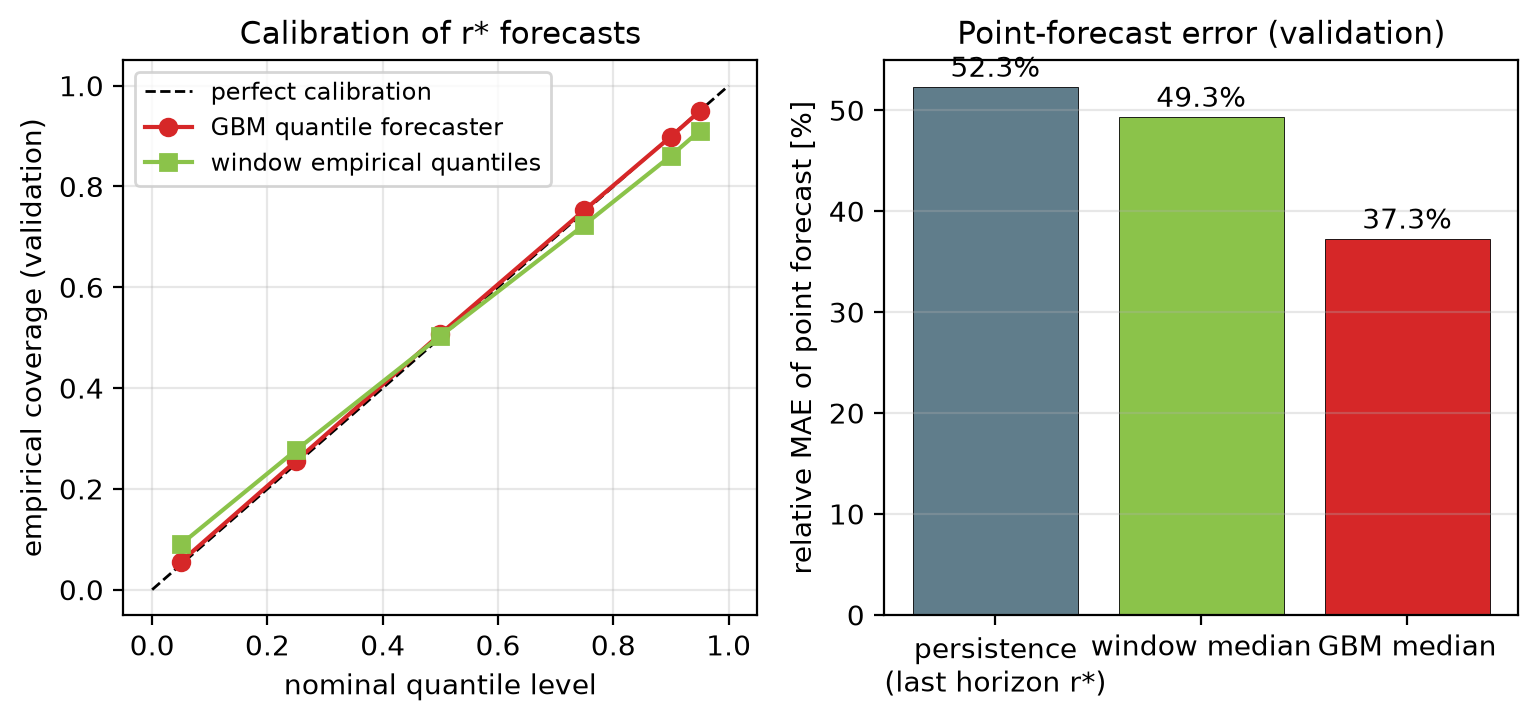
\includegraphics[width=0.95\linewidth]{fig5_forecast_quality.png}
    \end{column}
  \end{columns}
\end{frame}

\begin{frame}{Key idea 2: the KKT (constrained newsvendor) allocation rule}
  \small
  \textbf{Surrogate objective} (one interval, forecast distribution $F_i$ of $\rstar_i$):
  \[
    \max_{r}\ \sum_i w_i\,\mathbb{E}\big[\min(B_i + \rstar_i,\ r_i)\big]\quad \text{s.t.}\ \sum_i r_i \le C,\ 0\le r_i\le \mathrm{cap}_i
  \]
  $\mathbb{E}[\min(\cdot, r)]$ is concave with derivative $w_i\,(1 - F_i(r - B_i))$ = weighted probability that the marginal bit is needed. Separable concave $\Rightarrow$ KKT gives the global optimum:
  \[
    \boxed{\; r_i(\lambda) = \mathrm{clip}\Big(B_i + F_i^{-1}\big(1 - \lambda/w_i\big),\ 0,\ \mathrm{cap}_i\Big)\;}
  \]
  \begin{itemize}
    \item One scalar $\lambda \ge 0$ with $\sum_i r_i(\lambda) = C$: \textbf{60-step bisection}; $\lambda = 0$ if the link is not binding (surplus shared as headroom).
    \item $F_i^{-1}$: piecewise-linear through the 6 quantiles; cost $\mathcal{O}(NK + N n_{\rm iter})$, tens of $\mu$s for $N=8$.
  \end{itemize}
  \begin{exampleblock}{Intuition}
    Every cell is cut at the \textbf{same priority-weighted risk}. Wide forecast or high priority $\Rightarrow$ more margin; confident forecast $\Rightarrow$ about its median. Margins are \emph{derived}, not tuned.
  \end{exampleblock}
\end{frame}

\begin{frame}{Properties of the rule}
  \footnotesize
  \begin{columns}[T]
    \begin{column}{0.48\textwidth}
      \begin{block}{Proposition 1 (feasibility)}
        For any forecast and any $\lambda$, budgets satisfy the caps and $\sum_i r_i \le C$.
      \end{block}
    \end{column}
    \begin{column}{0.5\textwidth}
      \begin{block}{Proposition 3 (backlog first)}
        Any cell with $\lambda < w_i$ receives at least $\min(B_i,\mathrm{cap}_i)$ before uncertain demand of an equal- or lower-weight cell is funded.
      \end{block}
    \end{column}
  \end{columns}
  \begin{block}{Proposition 2 (equal weighted tail probability)}
    At an interior optimum $w_i\big(1 - F_i(r_i - B_i)\big) = \lambda$ for every cell. Point forecasts (degenerate $F_i$) reduce the rule to a priority-ordered fill.
  \end{block}
  \begin{block}{Proposition 4 (robustness to miscalibration)}
    If $\sup_x |F_i(x) - G_i(x)| \le \epsilon$ (Kolmogorov) for every cell, then
    \[
      J_G(r^G) - J_G(r^F) \le \epsilon\sum_i w_i\big[(r_i^G - B_i)^+ + (r_i^F - B_i)^+\big] \le 2\,\epsilon\, w_{\max}\, C.
    \]
    Loss from a miscalibrated forecast grows at most \textbf{linearly} in $\epsilon$.
  \end{block}
\end{frame}

\begin{frame}{Control loop}
  \centering
  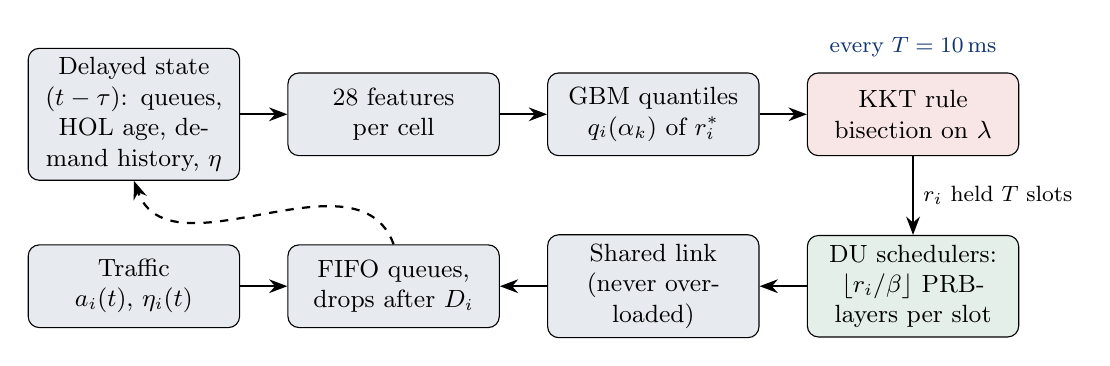
\begin{tikzpicture}[font=\small,>=Stealth,node distance=0.55cm and 0.6cm,
     st/.style={draw,rounded corners,fill=iitblue!10,align=center,minimum height=1.05cm,text width=2.45cm}]
    \node[st] (obs) {Delayed state\\ ($t-\tau$): queues, HOL age, demand history, $\eta$};
    \node[st,right=of obs] (feat) {28 features\\per cell};
    \node[st,right=of feat] (gbm) {GBM quantiles\\$q_i(\alpha_k)$ of $\rstar_i$};
    \node[st,right=of gbm,fill=accent!12] (kkt) {KKT rule\\bisection on $\lambda$};
    \node[st,below=1.0cm of kkt,fill=good!12] (du) {DU schedulers:\\$\lfloor r_i/\beta\rfloor$ PRB-layers per slot};
    \node[st,left=of du] (link) {Shared link\\(never overloaded)};
    \node[st,left=of link] (q) {FIFO queues,\\drops after $D_i$};
    \node[st,left=of q] (traffic) {Traffic\\$a_i(t)$, $\eta_i(t)$};
    \draw[->,thick] (obs) -- (feat);
    \draw[->,thick] (feat) -- (gbm);
    \draw[->,thick] (gbm) -- (kkt);
    \draw[->,thick] (kkt) -- node[right]{\footnotesize $r_i$ held $T$ slots} (du);
    \draw[->,thick] (du) -- (link);
    \draw[->,thick] (link) -- (q);
    \draw[->,thick] (traffic) -- (q);
    \draw[->,thick,dashed] (q.north) to[out=110,in=-70] (obs.south);
    \node[above=0.08cm of kkt,text=iitblue,font=\footnotesize] {every $T=10$\,ms};
  \end{tikzpicture}
  \vspace{0.6em}
  \begin{itemize}\small
    \item \textbf{Edge cases}: non-finite forecasts $\to$ window quantiles; zero demand $\to$ zero budget + headroom; link not binding $\to$ full predictive support.
    \item \textbf{Calibrated variant}: adaptive conformal offset $\delta_i \leftarrow \mathrm{clip}(\delta_i + \gamma(\mathbb 1[y_i > q_i(0.9)] - 0.1))$, reported as ablation.
  \end{itemize}
\end{frame}

\begin{frame}{Reference controllers (all tuned on validation seeds)}
  \footnotesize
  \centering
  \begin{tabular}{lll}
    \toprule
    Controller & Estimate of $\rstar$ & Allocation \\
    \midrule
    Static equal & none & $C/N$ \\
    Reactive proportional & mean-rate EWMA (deadline-unaware) & proportional water-fill \\
    MaxWeight & priority $\times$ queue, HOL-age urgency & max-weight \\
    Deadline-aware reactive & persistence: last observed $\rstar$ & deadline-weighted water-fill \\
    Point forecast & GBM \textbf{median} & deadline-weighted water-fill \\
    Fixed global quantile & GBM quantile, one tuned level (0.75) & water-fill \\
    Proposed (window) & empirical quantiles, last 30 horizons (\textbf{no ML}) & KKT rule \\
    \textbf{Proposed} & \textbf{GBM quantiles} & \textbf{KKT rule} \\
    Proposed + ACI & GBM quantiles + conformal offset & KKT rule \\
    Oracle water-fill & true $\rstar$ (not implementable) & water-fill \\
    Oracle + KKT & true $\rstar$ (not implementable) & KKT rule \\
    \bottomrule
  \end{tabular}
  \vspace{0.2em}
  \begin{itemize}
    \item Margins $\{0, 0.25, 0.5\}$, EWMA windows, persistence windows tuned; \textbf{margin 0 was best for all} (inflating a point estimate hurts under proportional shortage split).
    \item Every baseline redistributes unused capacity; same weights, backlog rate and water-fill as the point-forecast controller.
  \end{itemize}
\end{frame}

\begin{frame}{Evaluation protocol}
  \begin{columns}[T]
    \begin{column}{0.5\textwidth}
      \textbf{Family S} (synthetic, bursty)
      \begin{itemize}\small
        \item Gamma background + ON/OFF bursts with \textbf{Pareto sojourns} ($\alpha_{\rm on}=1.5$, $\alpha_{\rm off}=1.8$), slow regimes, SE drift
        \item Scenarios: low 0.50, moderate 0.65, high 0.80, flash crowds, \textbf{held-out shift} (never seen in training/tuning)
      \end{itemize}
      \textbf{Family G} (standards-based, nothing hand-designed)
      \begin{itemize}\small
        \item 3GPP TR 38.901 UMa, 7 interfering sites, Jakes fading, TS 38.214 CQI table
        \item eMBB: FTP Model 3; LL: XR video (TR 38.838, 60\,fps)
        \item Demand = output of a round-robin PRB scheduler
      \end{itemize}
    \end{column}
    \begin{column}{0.48\textwidth}
      \textbf{Protocol}
      \begin{itemize}\small
        \item 20 test seeds $\times$ 20{,}000 slots (10\,s) after 1{,}000 warm-up
        \item \textbf{Identical traces} and identical stale observations for all controllers
        \item Separate train / validation / test seeds; forecaster frozen before test
        \item Paired per-seed comparison: bootstrap 95\,\% CI, \textbf{Holm-corrected Wilcoxon} tests
        \item Ablations: point vs.\ quantile, ML vs.\ non-ML, calibration on/off, $T$, $\tau$, miscalibration, priority weight
      \end{itemize}
      \textbf{Supporting metrics}: per-class violations, utilisation, unused allocation, DU delay, Jain fairness, decision time.
    \end{column}
  \end{columns}
\end{frame}

% =====================================================================
\section{Part B: Results}
% =====================================================================

\begin{frame}{Main result, Family S: $V_w$ [\%] (mean $\pm$ std, 20 seeds)}
  \scriptsize
  \centering
  \begin{tabular}{lccccc}
    \toprule
    Method & low 0.50 & moderate 0.65 & high 0.80 & flash crowds & shift (held-out) \\
    \midrule
    Static equal share & 4.45 $\pm$ 1.05 & 9.65 $\pm$ 1.36 & 15.46 $\pm$ 1.51 & 19.15 $\pm$ 2.34 & 22.31 $\pm$ 2.99 \\
    Reactive proportional & 0.83 $\pm$ 0.27 & 4.11 $\pm$ 0.69 & 9.20 $\pm$ 0.99 & 12.27 $\pm$ 2.23 & 11.70 $\pm$ 2.24 \\
    MaxWeight & 0.90 $\pm$ 0.28 & 4.85 $\pm$ 0.79 & 11.54 $\pm$ 1.27 & 15.24 $\pm$ 3.02 & 12.31 $\pm$ 2.44 \\
    Deadline-aware reactive & 0.52 $\pm$ 0.21 & 4.24 $\pm$ 0.78 & 11.03 $\pm$ 1.33 & 14.51 $\pm$ 3.06 & 12.56 $\pm$ 2.81 \\
    Point forecast (GBM median) & 0.27 $\pm$ 0.17 & 3.23 $\pm$ 0.73 & 9.70 $\pm$ 1.34 & 13.33 $\pm$ 3.09 & 11.30 $\pm$ 2.81 \\
    Fixed global quantile (0.75) & 0.34 $\pm$ 0.23 & 4.35 $\pm$ 1.02 & 11.76 $\pm$ 1.44 & 15.09 $\pm$ 3.17 & 12.85 $\pm$ 3.32 \\
    Proposed, window quantiles (no ML) & 0.25 $\pm$ 0.13 & 2.57 $\pm$ 0.64 & 8.72 $\pm$ 1.34 & 12.67 $\pm$ 3.19 & 10.22 $\pm$ 2.88 \\
    \rowcolor{good!15}\textbf{Proposed (GBM quantiles + KKT)} & \textbf{0.15 $\pm$ 0.13} & \textbf{2.15 $\pm$ 0.60} & \textbf{8.00 $\pm$ 1.27} & \textbf{11.76 $\pm$ 3.08} & \textbf{10.04 $\pm$ 2.71} \\
    Proposed + ACI calibration & 0.17 $\pm$ 0.13 & 2.17 $\pm$ 0.61 & 8.14 $\pm$ 1.30 & 12.27 $\pm$ 3.26 & 11.12 $\pm$ 3.22 \\
    \midrule
    \textcolor{gray}{Oracle water-fill (not implementable)} & \textcolor{gray}{0.07} & \textcolor{gray}{1.62} & \textcolor{gray}{6.89} & \textcolor{gray}{10.16} & \textcolor{gray}{6.69} \\
    \bottomrule
  \end{tabular}
  \normalsize
  \vspace{0.6em}
  \begin{itemize}
    \item The proposed rule is the \textbf{best implementable controller in all 5 scenarios}.
    \item Std across seeds is dominated by burst timing that all methods share $\Rightarrow$ the \textbf{paired} comparison is the right reading (next slide).
  \end{itemize}
\end{frame}

\begin{frame}{Paired per-seed reduction by the proposed rule (Family S)}
  \scriptsize
  \centering
  Mean relative change of $V_w$ [95\,\% bootstrap CI], seeds won /20; ** Holm-Wilcoxon $p<0.01$, * $p<0.05$\\[4pt]
  \begin{tabular}{lccccc}
    \toprule
    Proposed vs. & low & moderate & high & flash crowds & shift \\
    \midrule
    Reactive prop. & $-81$\,\% 20/20** & $-48$\,\% 20/20** & $-13$\,\% 20/20** & \hl{$-4$\,\% 16/20*} & $-14$\,\% 20/20** \\
    MaxWeight & $-83$\,\% 20/20** & $-56$\,\% 20/20** & $-31$\,\% 20/20** & $-23$\,\% 20/20** & $-18$\,\% 20/20** \\
    Deadline-aware reactive & $-70$\,\% 20/20** & $-49$\,\% 20/20** & $-27$\,\% 20/20** & $-19$\,\% 20/20** & $-20$\,\% 20/20** \\
    Point forecast & $-43$\,\% 20/20** & $-33$\,\% 20/20** & $-18$\,\% 20/20** & $-12$\,\% 20/20** & $-11$\,\% 20/20** \\
    Fixed global quantile & $-54$\,\% 20/20** & $-50$\,\% 20/20** & $-32$\,\% 20/20** & $-22$\,\% 20/20** & $-22$\,\% 20/20** \\
    Window quantiles (no ML) & $-37$\,\% 20/20** & $-16$\,\% 20/20** & $-8$\,\% 20/20** & $-7$\,\% 20/20** & \hl{$-2$\,\% 16/20**} \\
    + ACI calibration & $-9$\,\% 18/20** & $-1$\,\% 16/20** & $-2$\,\% 19/20** & $-4$\,\% 20/20** & $-10$\,\% 20/20** \\
    \bottomrule
  \end{tabular}
  \normalsize
  \vspace{0.5em}
  \begin{columns}[T]
    \begin{column}{0.5\textwidth}
      \begin{exampleblock}{Supported}
        \small vs.\ point forecast, fixed quantile, MaxWeight and deadline-aware reactive: every scenario incl.\ held-out shift, \textbf{every seed}, $p<0.01$.
      \end{exampleblock}
    \end{column}
    \begin{column}{0.5\textwidth}
      \begin{alertblock}{Weak}
        \small vs.\ reactive proportional under flash crowds ($-4$\,\%): it starves LL cells (17.8\,\% vs 4.6\,\%) but serves eMBB better.
      \end{alertblock}
    \end{column}
  \end{columns}
\end{frame}

\begin{frame}{Where the gain comes from (scenario high, 20 seeds)}
  \begin{columns}[c]
    \begin{column}{0.56\textwidth}
      \scriptsize
      \begin{tabular}{lcccc}
        \toprule
        Method & LL viol. & eMBB viol. & util. & Jain \\
        \midrule
        Reactive prop. & 14.7\,\% & 4.0\,\% & 74.7\,\% & 0.996 \\
        MaxWeight & 20.6\,\% & 2.9\,\% & 74.1\,\% & 0.991 \\
        Deadline-aware react. & 5.2\,\% & 16.5\,\% & 69.3\,\% & 0.995 \\
        Point forecast & 3.1\,\% & 16.0\,\% & 70.1\,\% & 0.994 \\
        Fixed global quantile & 0.9\,\% & 22.0\,\% & 67.0\,\% & 0.985 \\
        \rowcolor{good!15}\textbf{Proposed} & 3.4\,\% & \textbf{12.3\,\%} & \textbf{72.2\,\%} & 0.997 \\
        Oracle water-fill & 0.04\,\% & 13.4\,\% & 72.3\,\% & 0.994 \\
        \bottomrule
      \end{tabular}
      \normalsize
      \begin{itemize}\small
        \item Deadline-unaware controllers sacrifice LL cells: large queues $\neq$ urgent queues.
        \item In the deadline-aware family the proposed rule has the \textbf{lowest eMBB loss and highest utilisation}: margin only where the forecast is wide.
        \item One global level over-protects LL and wastes 33\,\% of the allocation.
      \end{itemize}
    \end{column}
    \begin{column}{0.44\textwidth}
      \centering
      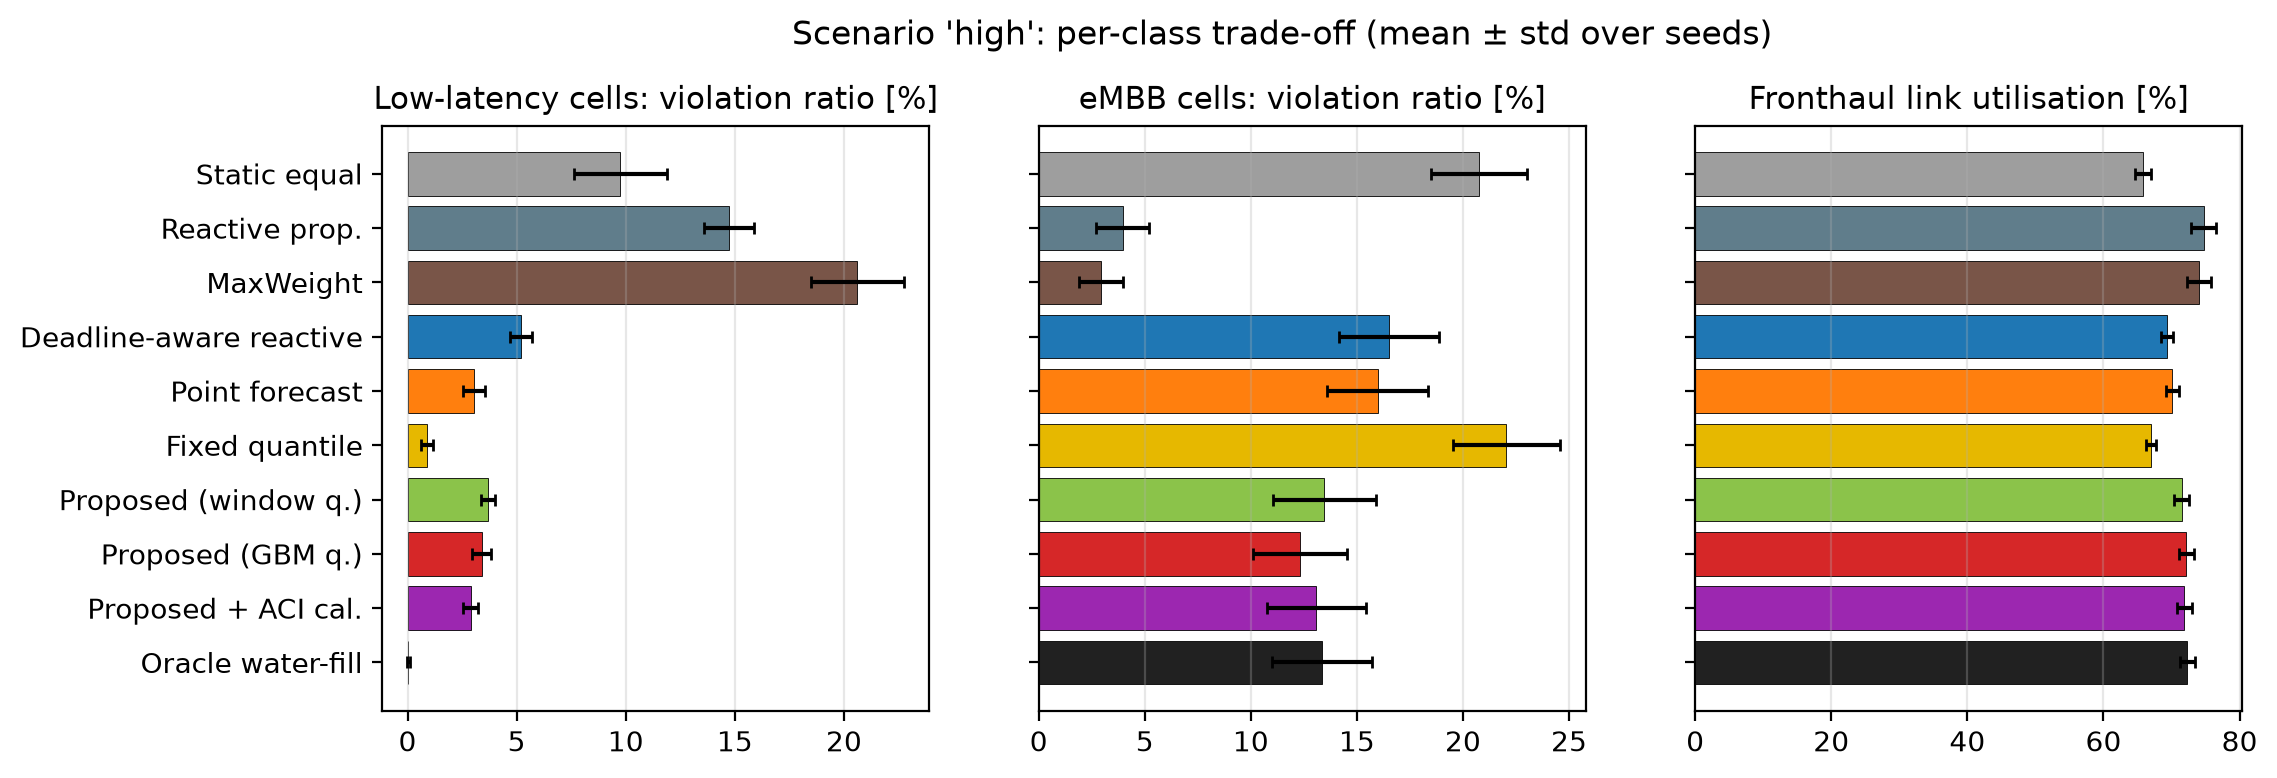
\includegraphics[width=\linewidth]{fig2_class_breakdown_high.png}
    \end{column}
  \end{columns}
\end{frame}

\begin{frame}{The rule in action: one low-latency cell}
  \begin{columns}[c]
    \begin{column}{0.62\textwidth}
      \centering
      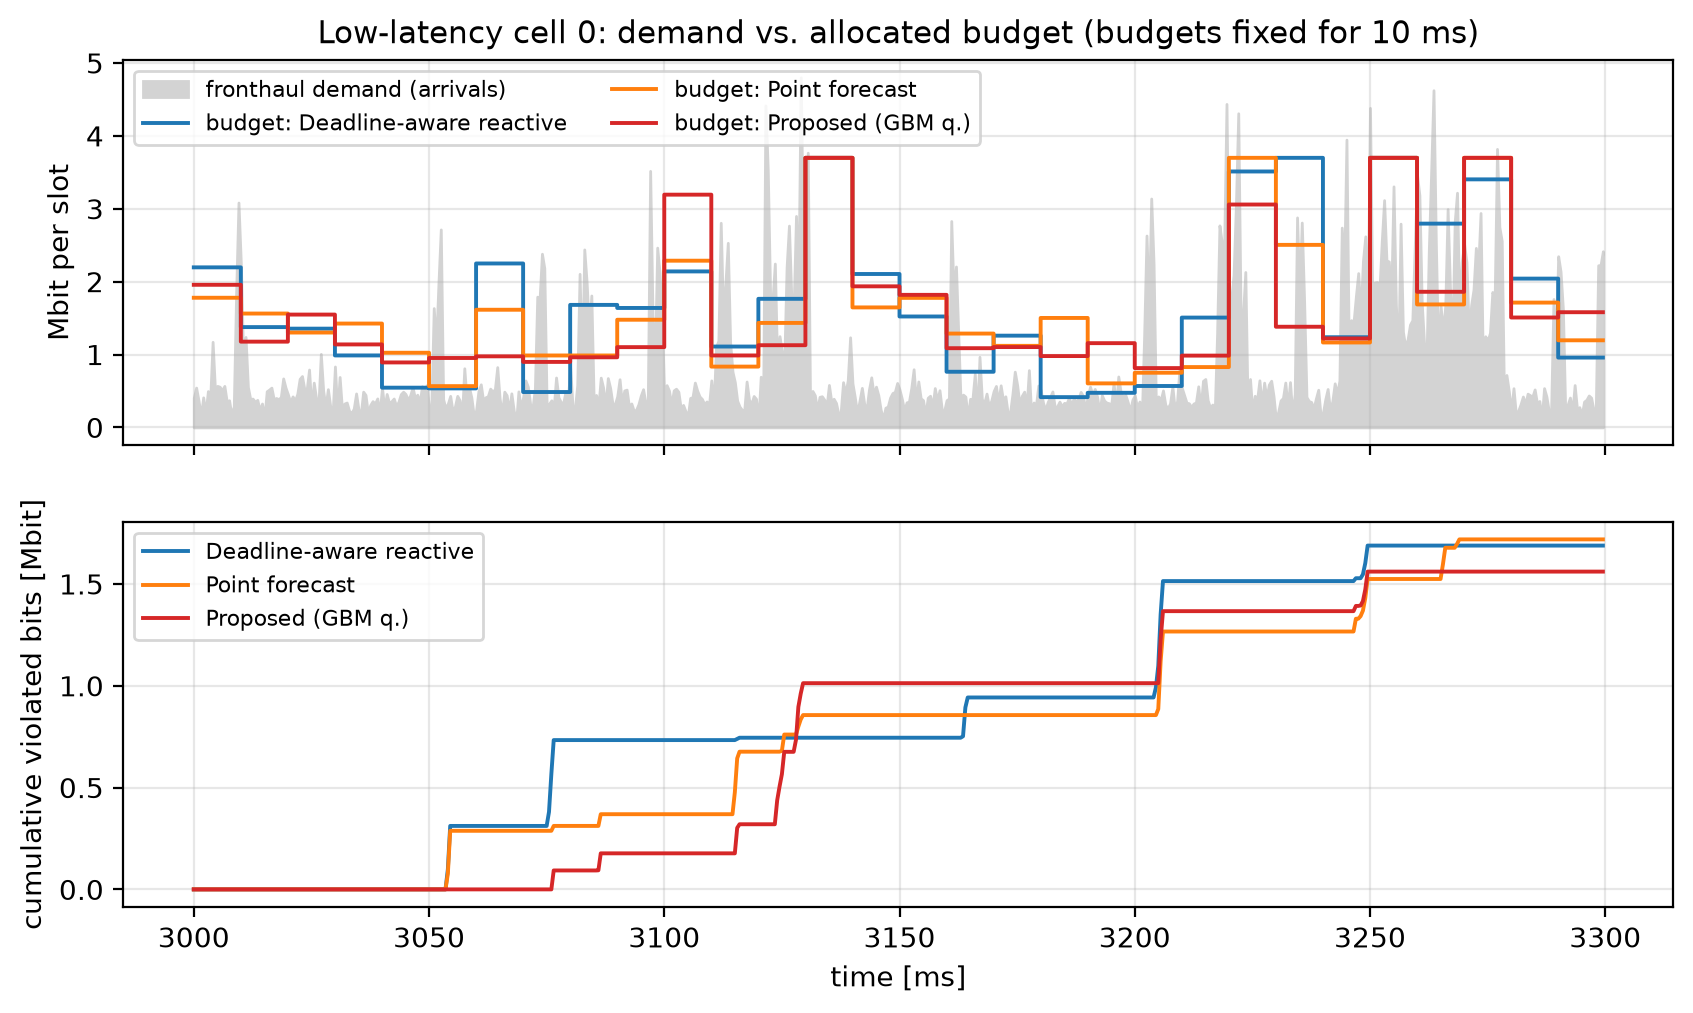
\includegraphics[width=\linewidth]{fig6_demo_timeseries.png}
    \end{column}
    \begin{column}{0.38\textwidth}
      \begin{itemize}
        \item Grey: demand; steps: budgets held for 10\,ms.
        \item The reactive controller is \textbf{one interval late} at every burst.
        \item The proposed rule raises the budget where the forecast range is \textbf{wide} (burst onset).
        \item Fewest cumulative violated bits over the trace.
      \end{itemize}
    \end{column}
  \end{columns}
\end{frame}

\begin{frame}{Ablations: what actually carries the gain?}
  \begin{enumerate}
    \item \textbf{Point vs.\ quantile forecast} (same model, same rule family):\\
      $-11$\,\% to $-43$\,\%, 20/20 seeds everywhere $\Rightarrow$ \textbf{representing uncertainty matters}.
    \item \textbf{Per-cell KKT level vs.\ one tuned global level} (same forecast):\\
      $-22$\,\% to $-54$\,\% $\Rightarrow$ the level must be chosen \textbf{per cell by the link constraint}.
    \item \textbf{ML vs.\ non-ML quantiles} under the same KKT rule:\\
      GBM adds $-7$\,\% to $-37$\,\% on nominal traffic but only $-2$\,\% under the held-out shift.\\
      $\Rightarrow$ most of the gain is the \textbf{rule} ($\rstar$ target + KKT split), not the model. ML is \emph{useful}, not \emph{necessary}.
    \item \textbf{Online ACI calibration}: \hl{no gain} (1--9\,\% worse nominal, 10\,\% worse under shift).\\
      In a coupled allocation LL misses are partly \emph{caused} by the shortage split $\Rightarrow$ offsets inflate LL reservations and starve eMBB. Per-stream conformal correction does not transfer.
  \end{enumerate}
\end{frame}

\begin{frame}{Family G: standards-based 3GPP traffic}
  \begin{columns}[T]
    \begin{column}{0.55\textwidth}
      \scriptsize
      \begin{tabular}{lccc}
        \toprule
        Method & mod.\ 0.65 & high 0.80 & unweighted (high) \\
        \midrule
        Static equal & 10.75 & 13.10 & 19.2 \\
        Reactive prop. & 12.05 & 15.94 & 15.0 \\
        MaxWeight & 17.51 & 25.79 & 19.7 \\
        Deadline-aware react. & 8.95 & 11.53 & 18.5 \\
        Point forecast & 6.00 & 8.98 & 16.6 \\
        Fixed quantile & 6.80 & 9.88 & 18.7 \\
        Window quantiles & 6.18 & 9.01 & 16.0 \\
        \rowcolor{good!15}\textbf{Proposed} & \textbf{5.08} & \textbf{8.01} & \textbf{14.4} \\
        Transfer (trained on S) & 6.99 & 9.89 & 14.3 \\
        \midrule
        \textcolor{gray}{Oracle + KKT} & \textcolor{gray}{3.47} & \textcolor{gray}{6.06} & \textcolor{gray}{11.1} \\
        \bottomrule
      \end{tabular}
    \end{column}
    \begin{column}{0.43\textwidth}
      \begin{itemize}\small
        \item Main result \textbf{reproduces on traffic we did not design}: best implementable at both loads, 20/20 seeds.
        \item At high load: $-11$\,\% vs.\ point forecast, $-31$\,\% vs.\ deadline-aware reactive, $-50$\,\% vs.\ reactive proportional.
        \item Here also best under the \textbf{unweighted} ratio.
        \item Forecaster transferred from Family S still beats every reactive controller, but not the in-family point forecast.
      \end{itemize}
    \end{column}
  \end{columns}
\end{frame}

\begin{frame}{How much is still forecast error? (oracle + KKT)}
  \begin{columns}[c]
    \begin{column}{0.48\textwidth}
      \small
      \centering
      \begin{tabular}{lccc}
        \toprule
        Scenario & Proposed & Oracle+KKT & Gap \\
        \midrule
        S low & 0.15 & 0.05 & 70\,\% \\
        S moderate & 2.15 & 0.88 & 59\,\% \\
        S high & 8.00 & 4.77 & 40\,\% \\
        S flash crowds & 11.76 & 8.10 & 31\,\% \\
        S shift & 10.04 & 5.84 & 42\,\% \\
        G moderate & 5.08 & 3.47 & 32\,\% \\
        G high & 8.01 & 6.06 & 24\,\% \\
        \bottomrule
      \end{tabular}
    \end{column}
    \begin{column}{0.5\textwidth}
      \begin{itemize}
        \item Oracle + KKT = same rule with a perfect forecast of $\rstar$.
        \item The gap is what a better forecaster could still buy: \textbf{24--40\,\% at high load}.
        \item The rest is the unavoidable cost of committing budgets for 10\,ms.
        \item At $T = 2$\,ms: oracle + KKT 1.91\,\% vs.\ oracle water-fill 6.89\,\% with the \emph{same} perfect information $\Rightarrow$ \textbf{the allocation rule matters as much as the forecast}.
        \item ``Oracle'' is a reference, \textbf{not} an upper bound.
      \end{itemize}
    \end{column}
  \end{columns}
\end{frame}

\begin{frame}{Honest caveat: the gain is a priority trade}
  \begin{columns}[T]
    \begin{column}{0.52\textwidth}
      \textbf{Unweighted} violation ratio, Family S [\%]\\[2pt]
      \scriptsize
      \begin{tabular}{lccc}
        \toprule
        Method & moderate & high & flash \\
        \midrule
        Reactive prop. & \best{2.44} & \best{6.55} & \best{9.64} \\
        MaxWeight & 2.73 & 7.18 & 10.44 \\
        Point forecast & 3.93 & 12.88 & 17.62 \\
        Proposed ($w_{\rm LL}=3$) & 2.50 & 10.19 & 15.08 \\
        \bottomrule
      \end{tabular}\\[6pt]
      \normalsize
      \textbf{LL weight sweep}, $V_w$ [\%], S high\\[2pt]
      \scriptsize
      \begin{tabular}{lcccc}
        \toprule
        $w_{\rm LL}$ & 1 & 2 & 3 & 5 \\
        \midrule
        Reactive prop. & \best{6.55} & \best{8.13} & 9.20 & 10.56 \\
        Point forecast & 6.77 & 8.90 & 9.70 & 10.57 \\
        Proposed & 6.58 & 8.35 & \best{8.00} & \best{6.93} \\
        \bottomrule
      \end{tabular}
    \end{column}
    \begin{column}{0.46\textwidth}
      \begin{itemize}\small
        \item Under the unweighted ratio, plain proportional sharing loses fewer total bits at moderate/high load (it sacrifices the small LL cells).
        \item The rule matches proportional at $w_{\rm LL}=1$ and pulls ahead from $w_{\rm LL}=3$.
        \item Family G, $w_{\rm LL}=1$: rule is \emph{worse} than point forecast (15.9 vs 10.4\,\%) --- zero-inflated XR/FTP demand gives an all-or-nothing newsvendor allocation.
      \end{itemize}
      \begin{alertblock}{Scope of the claim}
        \small For operators who value a low-latency bit at least \textbf{2--3$\times$} an eMBB bit.
      \end{alertblock}
    \end{column}
  \end{columns}
\end{frame}

\begin{frame}{Sensitivity: control interval $T$ and telemetry delay $\tau$}
  \begin{columns}[c]
    \begin{column}{0.55\textwidth}
      \centering
      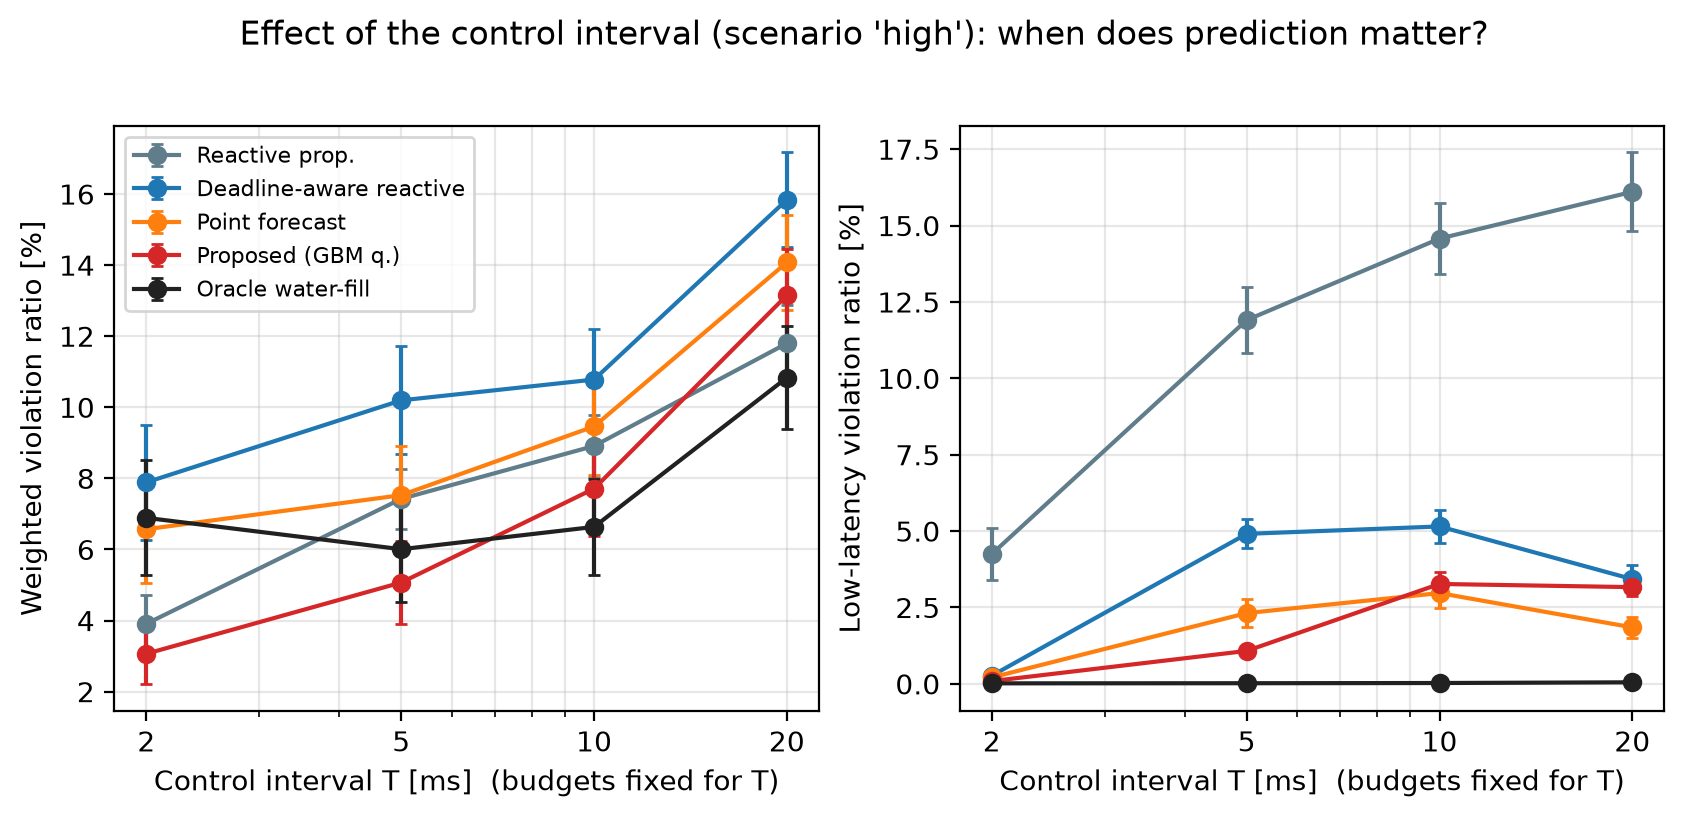
\includegraphics[width=\linewidth]{fig4_interval_sweep.png}
    \end{column}
    \begin{column}{0.45\textwidth}
      \scriptsize
      \begin{tabular}{lccc}
        \toprule
        $T$ & React.\ prop. & Point f. & Proposed \\
        \midrule
        2\,ms & 3.91 & 6.57 & \best{3.07} \\
        5\,ms & 7.42 & 7.53 & \best{5.07} \\
        10\,ms & 8.91 & 9.46 & \best{7.71} \\
        20\,ms & \best{11.80} & 14.08 & 13.15 \\
        \midrule
        $\tau$ & & & vs.\ react.\ prop. \\
        \midrule
        0\,ms & 8.16 & 8.45 & 6.85 ($-16$\,\%) \\
        1\,ms & 8.91 & 9.46 & 7.71 ($-13$\,\%) \\
        2.5\,ms & 9.86 & 10.51 & 8.77 ($-11$\,\%) \\
        5\,ms & 11.30 & 12.45 & 11.07 ($-2$\,\%) \\
        \bottomrule
      \end{tabular}
      \normalsize
      \begin{itemize}\small
        \item Short $T$: rule beats even the oracle water-fill.
        \item $T = 20$\,ms ($5\times$ LL deadline) or $\tau = 5$\,ms: advantage over proportional vanishes.
      \end{itemize}
    \end{column}
  \end{columns}
\end{frame}

\begin{frame}{Robustness to forecast miscalibration (Prop.~4 in practice)}
  \begin{columns}[c]
    \begin{column}{0.5\textwidth}
      \centering
      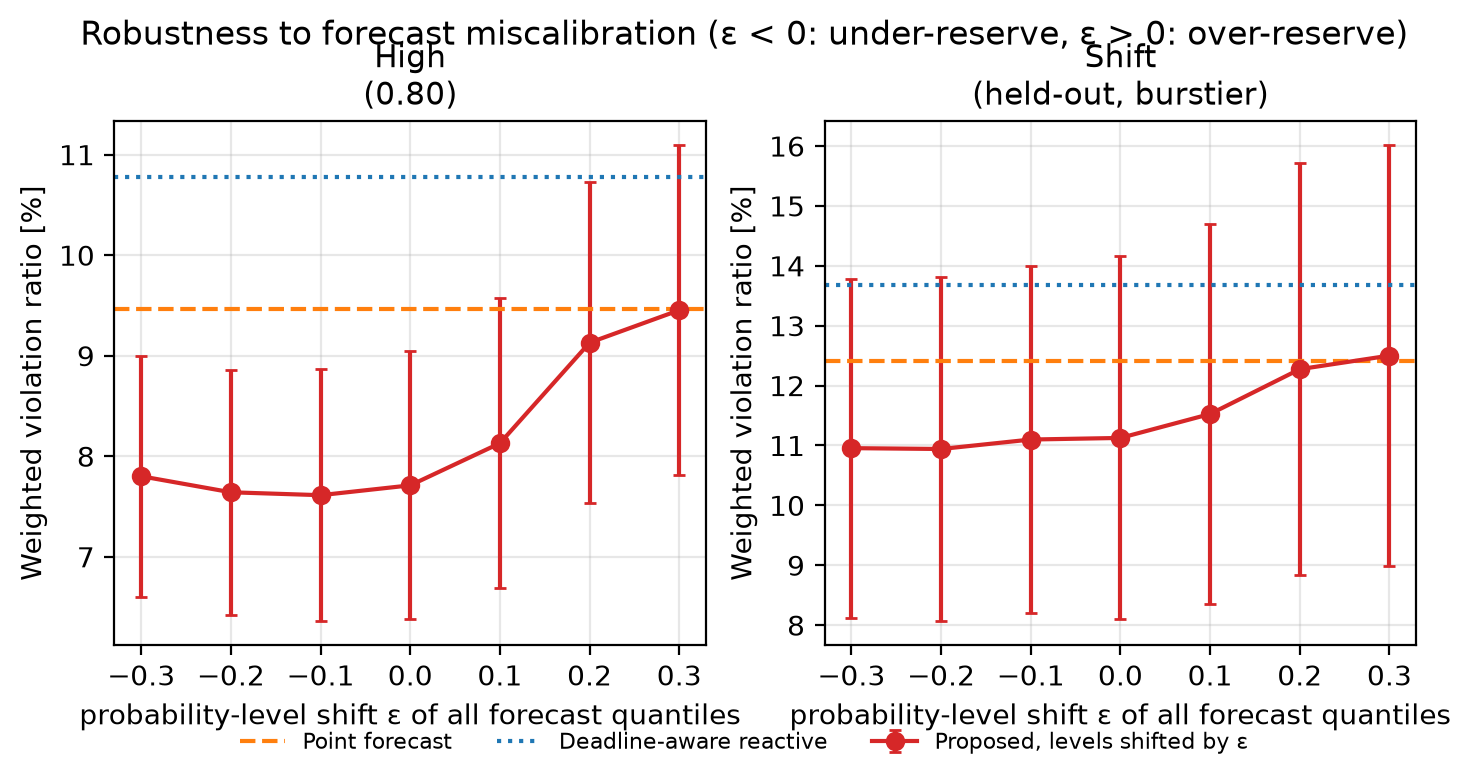
\includegraphics[width=\linewidth]{fig10_miscalibration.png}
    \end{column}
    \begin{column}{0.5\textwidth}
      Every forecast quantile level shifted by $\epsilon$ before allocation:\\[3pt]
      \scriptsize
      \begin{tabular}{lccccc}
        \toprule
        $\epsilon$ & $-0.3$ & $-0.1$ & 0 & $+0.1$ & $+0.3$ \\
        \midrule
        high & 7.80 & 7.61 & 7.71 & 8.13 & 9.45 \\
        shift & 10.96 & 11.10 & 11.13 & 11.53 & 12.50 \\
        \bottomrule
      \end{tabular}\\[2pt]
      Point forecast: 9.46 / 12.42;\ deadline-aware: 10.78 / 13.68\\
      \normalsize
      \begin{itemize}\small
        \item Under-reserving is almost harmless: a common shift is absorbed by $\lambda$.
        \item Over-reserving degrades gradually (+23\,\% at $\epsilon=0.3$).
        \item Even then the rule matches the point forecast and beats deadline-aware reactive.
      \end{itemize}
    \end{column}
  \end{columns}
\end{frame}

\begin{frame}{Part A $\times$ Part B: compression width vs.\ allocation rule}
  \begin{columns}[c]
    \begin{column}{0.58\textwidth}
      \centering
      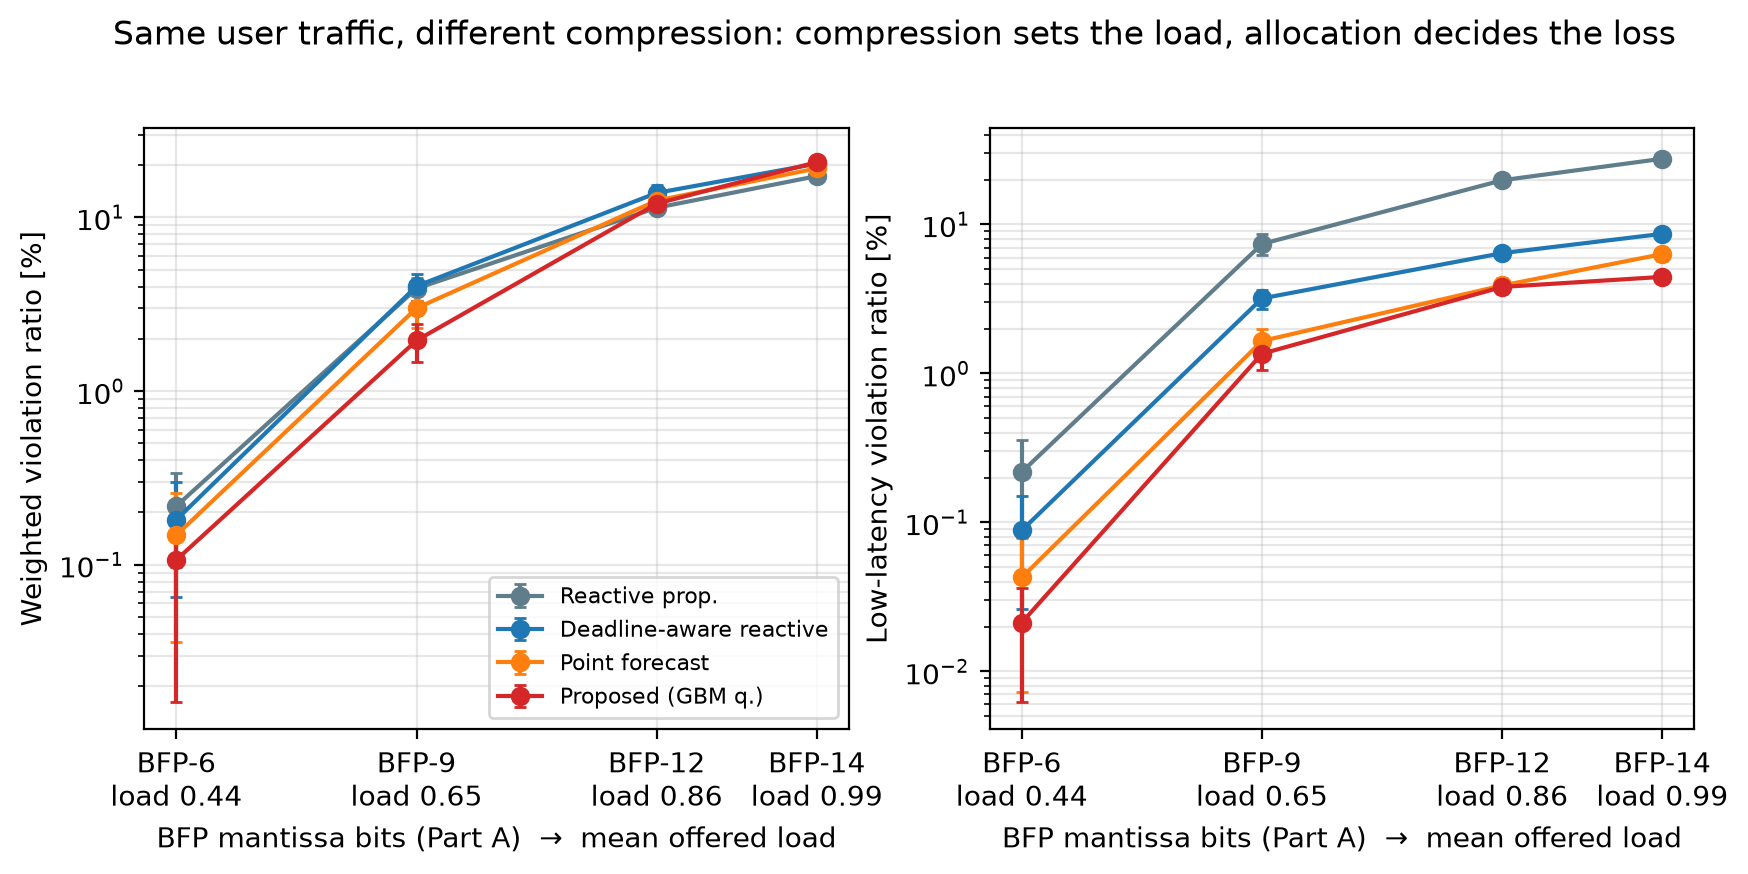
\includegraphics[width=\linewidth]{fig9_compression_vs_allocation.png}
    \end{column}
    \begin{column}{0.42\textwidth}
      \scriptsize
      Same user traffic; only BFP width changes $\beta$\\[2pt]
      \begin{tabular}{lcccc}
        \toprule
        BFP & load & React. & Point & Prop. \\
        \midrule
        6 bit & 0.44 & 0.22 & 0.15 & \best{0.11} \\
        9 bit & 0.65 & 3.90 & 3.00 & \best{1.96} \\
        12 bit & 0.86 & \best{11.37} & 12.50 & 12.01 \\
        14 bit & 0.99 & \best{17.29} & 19.16 & 20.81 \\
        \bottomrule
      \end{tabular}
      \normalsize
      \begin{itemize}\small
        \item \textbf{Compression sets the regime}; allocation decides the loss inside it.
        \item Allocation matters most at load $\approx$ \textbf{0.5--0.8} (half the loss at 0.65).
        \item At $\approx 1.0$ load no split helps: need more compression or capacity.
      \end{itemize}
    \end{column}
  \end{columns}
\end{frame}

\begin{frame}{Decision overhead}
  \begin{columns}[c]
    \begin{column}{0.5\textwidth}
      \centering
      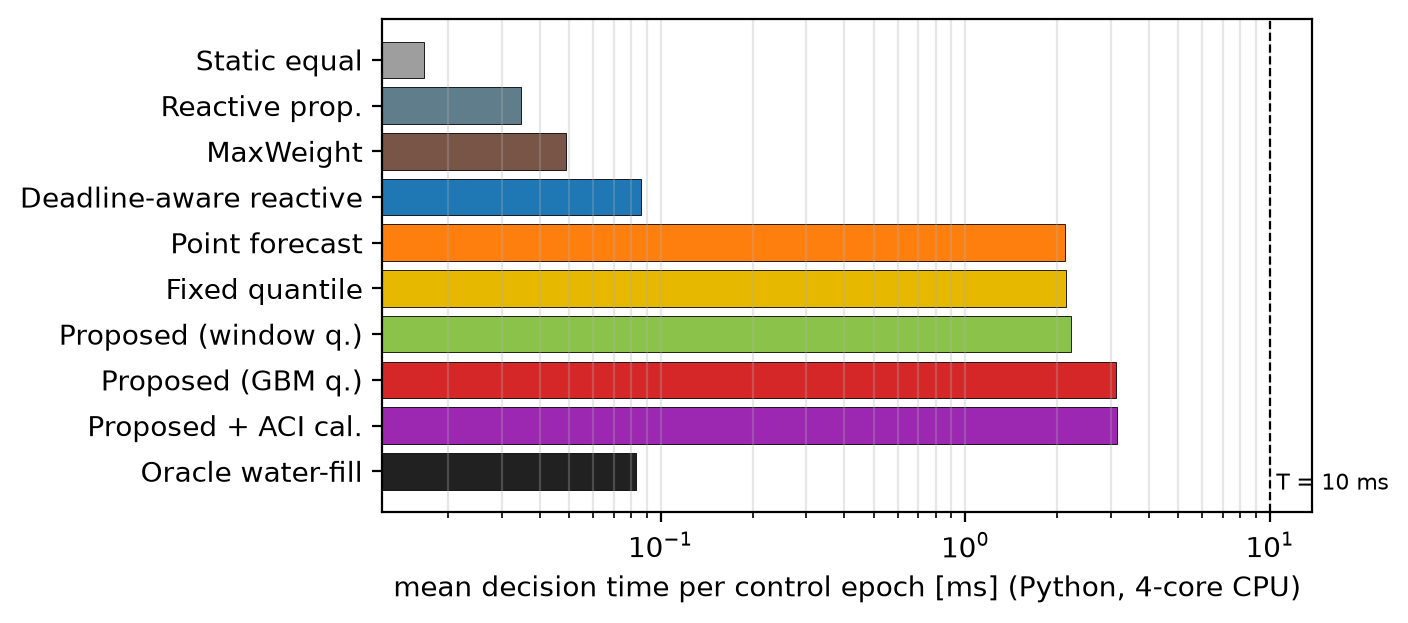
\includegraphics[width=\linewidth]{fig7_decision_time.png}
    \end{column}
    \begin{column}{0.5\textwidth}
      Python, 4-core CPU, per 10\,ms control epoch:
      \begin{itemize}\small
        \item Static 0.02\,ms, reactive prop.\ 0.04\,ms, MaxWeight 0.05\,ms, deadline-aware 0.09\,ms
        \item Window quantiles 2.2\,ms, point forecast 2.5\,ms, \textbf{proposed 3.5\,ms}
      \end{itemize}
      \begin{itemize}\small
        \item The KKT rule itself: $< 0.1$\,ms.
        \item Cost = features + $6 \times 300$ trees; vectorised numpy tree traversal (1.8\,ms vs.\ 12\,ms for scikit-learn \texttt{predict}).
        \item Real O-DU: compiled (C++/numba) model or the no-ML window-quantile fallback.
      \end{itemize}
    \end{column}
  \end{columns}
\end{frame}

% =====================================================================
\section{Extended Study: Theory and Stronger Controllers}
% =====================================================================

\begin{frame}{The real control problem: a POMDP}
  \small
  State $s(t) = (Q(t), Z(t), \eta(t))$: queue age profiles, hidden traffic state, spectral efficiency. At epochs $t_k = kT$:
  \[
    \min_{\pi}\ \mathbb{E}_\pi\Big[\sum_k \sum_{t=t_k}^{t_k+T-1} \sum_i w_i^{\rm p}\,\mathrm{dropped}_i(t)\Big],
    \qquad r(t_k) = \pi\big(s(t_k - \tau),\text{history}\big)
  \]
  \textbf{Intractable}: continuous state of dimension in the hundreds, unknown traffic law, action held for $T$ slots.\\[4pt]
  Three approximation families, all implemented:
  \begin{enumerate}
    \item \textbf{One-step stochastic programs} (certainty-equivalent / rollout): the KKT newsvendor rule on a learned or model-based distribution.
    \item \textbf{Lyapunov drift}: MaxWeight; \textbf{predictive MaxWeight} (Huang et al.\ 2016) with queue $+$ look-ahead $\times$ forecast median.
    \item \textbf{Direct policy search}: 3-parameter class-level policy learned by the \textbf{cross-entropy method} (CEM) --- small analogue of a DRL xApp.
  \end{enumerate}
  Plus a third traffic family \textbf{M}: Markov-modulated Gamma sources (idle/normal/burst), with a \textbf{semi-Markov held-out shift} (Pareto sojourns).
\end{frame}

\begin{frame}{Markov-fluid theory of the deadline-feasible rate}
  \footnotesize
  Phase chain $P$ (stationary $\pi$), per-phase log-MGF $\psi_k(\theta)$, $\Phi(\theta) = \mathrm{diag}(e^{\psi_k(\theta)})$.
  \begin{itemize}
    \item Window log-MGF: $\Lambda_l(\theta) = \log\big(\pi^{\mathsf T}\Phi(P\Phi)^{l-1}\mathbf 1\big)$;\quad effective bandwidth $\alpha(\theta) = \log\rho(P\Phi(\theta))/\theta$.
    \item \textbf{Chernoff-union bound}: $\Pr(\rstar > x) \le \sum_{l=1}^{H}(H-l+1)\min_\theta \exp\big(-\theta x(l+D) + \Lambda_l(\theta)\big)$.
    \item \textbf{Large-deadline decay}: $\limsup_{D\to\infty} D^{-1}\log\Pr(\rstar > x) \le -x\,\theta^\ast(x)$ --- links $\rstar$ to classical buffer-overflow asymptotics.
    \item \textbf{Shortfall sandwich} (pathwise, any arrivals): $(D+1)(\rstar - r)^+ \le V(r) \le \sum_t (a_t - r)^+$.\\
      $\Rightarrow$ the newsvendor surrogate is a \emph{lower} bound on violated volume.
  \end{itemize}
  \centering
  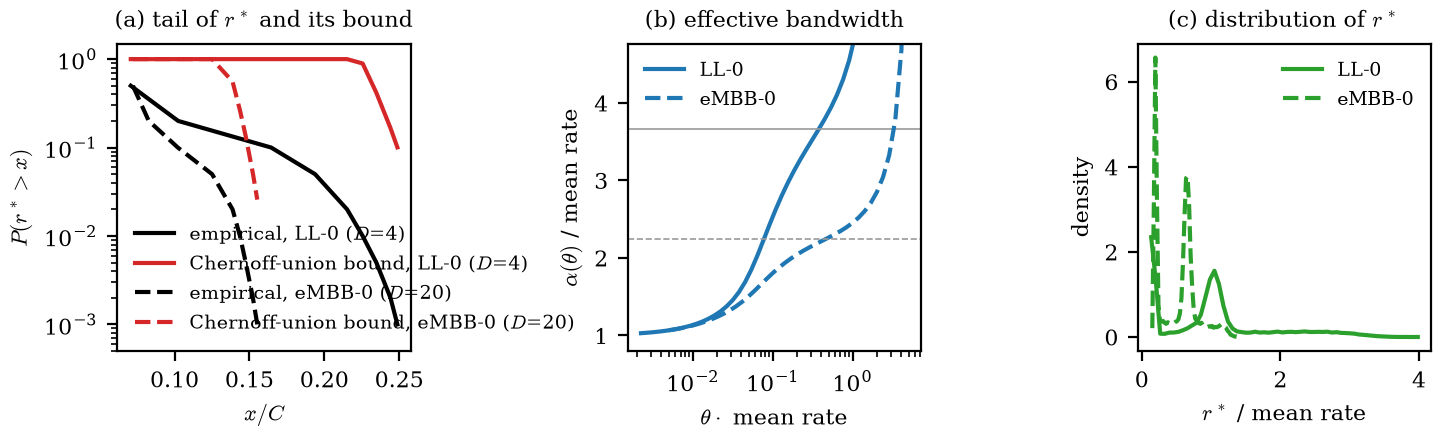
\includegraphics[width=0.72\linewidth]{paper_fig_theory.png}\\
  \footnotesize Validation (Family M, 20k horizons): sandwich never violated; bound valid but \textbf{25--100$\times$ conservative} at 2--10\,ms deadlines $\Rightarrow$ argument for \emph{learning} the distribution.
\end{frame}

\begin{frame}{Three families, nineteen controllers}
  \centering
  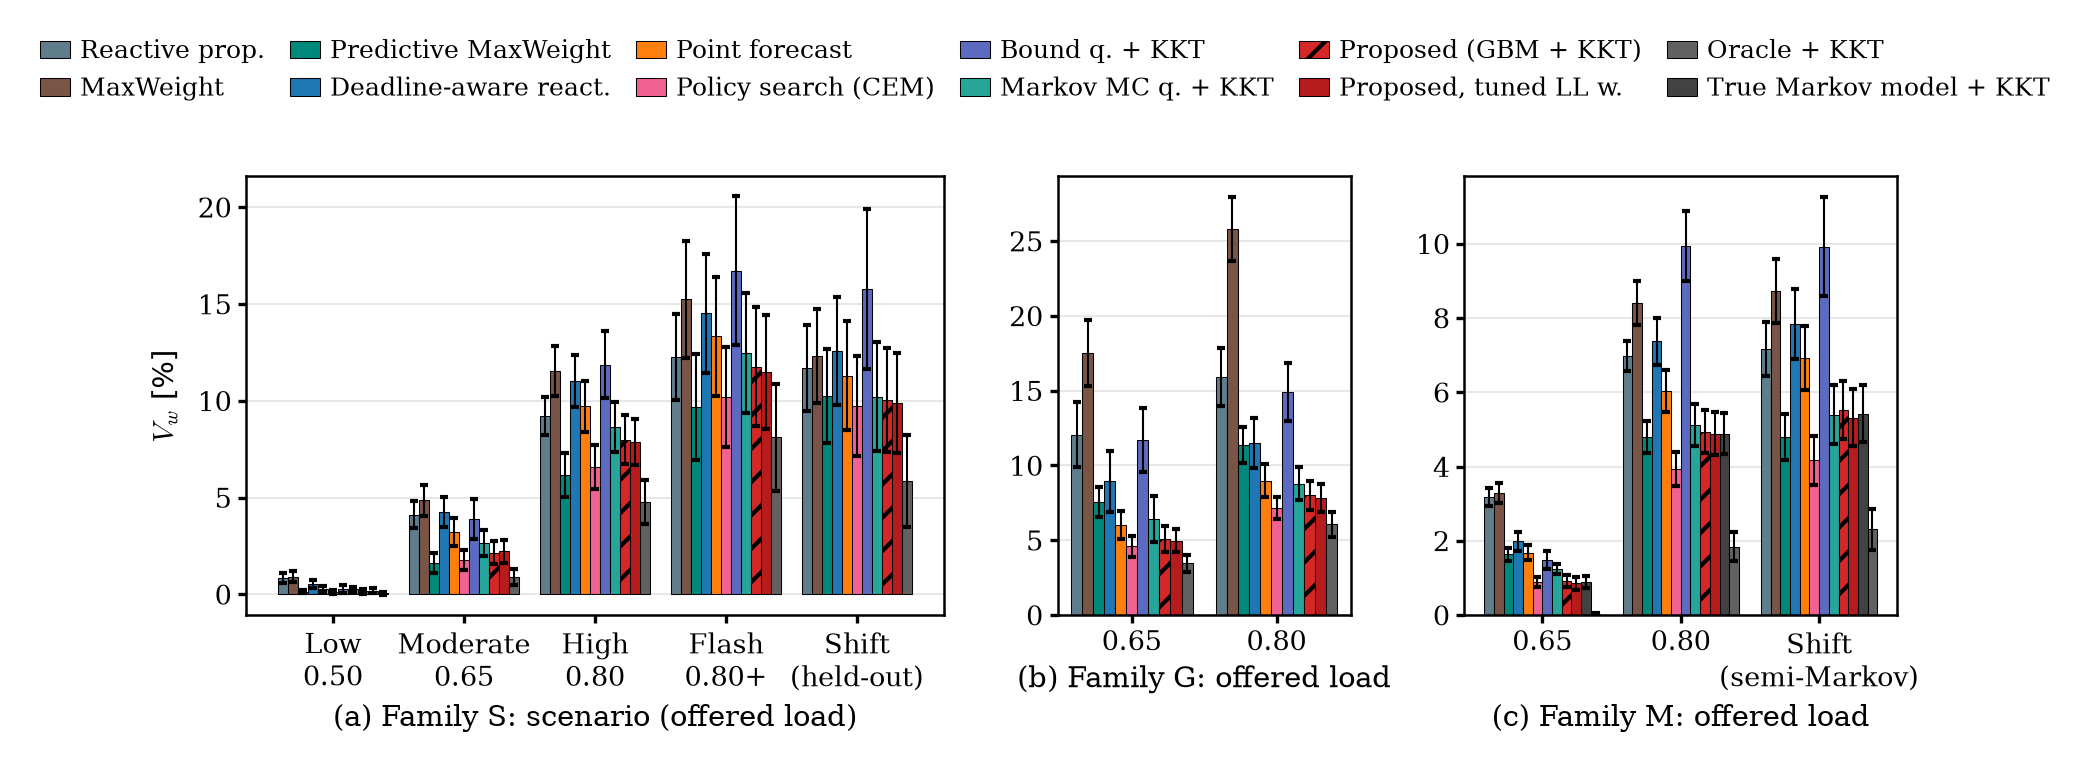
\includegraphics[width=0.95\linewidth]{paper_fig_overview_ext.png}
\end{frame}

\begin{frame}{Extended results: best implementable controller ($V_w$ [\%])}
  \scriptsize
  \centering
  \begin{tabular}{lccccc}
    \toprule
    Scenario & GBM + KKT & Pred.\ MaxWeight & CEM policy & Markov-chain KKT & Tuned-$w$ KKT \\
    \midrule
    S low 0.50 & 0.15 & 0.14 & \best{0.13} & 0.25 & 0.18 \\
    S moderate 0.65 & 2.15 & \best{1.62} & 1.77 & 2.65 & 2.21 \\
    S high 0.80 & 8.00 & \best{6.15} & 6.57 & 8.64 & 7.88 \\
    S flash crowd & 11.76 & \best{9.69} & 10.20 & 12.44 & 11.49 \\
    S shift & 10.04 & 10.25 & \best{9.73} & 10.22 & 9.90 \\
    G moderate 0.65 & 5.08 & 7.57 & \best{4.58} & 6.44 & 4.98 \\
    G high 0.80 & 8.01 & 11.36 & \best{7.17} & 8.77 & 7.83 \\
    M moderate 0.65 & 0.92 & 1.64 & 0.88 & 1.24 & \best{0.85} \\
    M high 0.80 & 4.94 & 4.79 & \best{3.93} & 5.12 & 4.88 \\
    M shift 0.80 & 5.52 & 4.80 & \best{4.17} & 5.39 & 5.31 \\
    \bottomrule
  \end{tabular}
  \normalsize
  \vspace{0.4em}
  \begin{itemize}\small
    \item Within the NCC comparison set the KKT rule still wins \textbf{all 10 scenarios} and is the best controller with \textbf{nothing to tune}.
    \item Two controllers using the \emph{same} forecaster beat it: \textbf{CEM policy} best in 6/10, \textbf{predictive MaxWeight} in 3/10 (all bursty Family S), tuned-weight KKT in 1/10.
    \item Markov chain fitted online (no training data) is within 3--9\,\% of the learned rule.
  \end{itemize}
\end{frame}

\begin{frame}{Why does re-tuning the LL weight not close the gap?}
  \footnotesize
  \begin{columns}[T]
    \begin{column}{0.5\textwidth}
      \textbf{KKT multiplier diagnostic} (high load, 3 seeds $\times$ 8000 slots)\\[3pt]
      \small
      \begin{tabular}{lccc}
        \toprule
        & S & G & M \\
        \midrule
        Link binding & 99.8\,\% & 100\,\% & 99.9\,\% \\
        $\lambda^\ast \ge w_{\rm eMBB}$ & 58\,\% & 56\,\% & 50\,\% \\
        \bottomrule
      \end{tabular}
      \normalsize
      \begin{itemize}\small
        \item In half the epochs every eMBB cell already sits at its lowest quantile: the weight has nothing left to move.
        \item Tuned weight: 8.00$\to$7.88 (S), 8.01$\to$7.83 (G) --- an order less than CEM.
        \item CEM gain comes from \textbf{decoupled per-class levels} ($p_{\rm LL}\!\approx\!0.8$, $p_{\rm eMBB}\!\approx\!0.5$) and a different sharing rule: \textbf{structure}, not the constant.
      \end{itemize}
    \end{column}
    \begin{column}{0.5\textwidth}
      \centering
      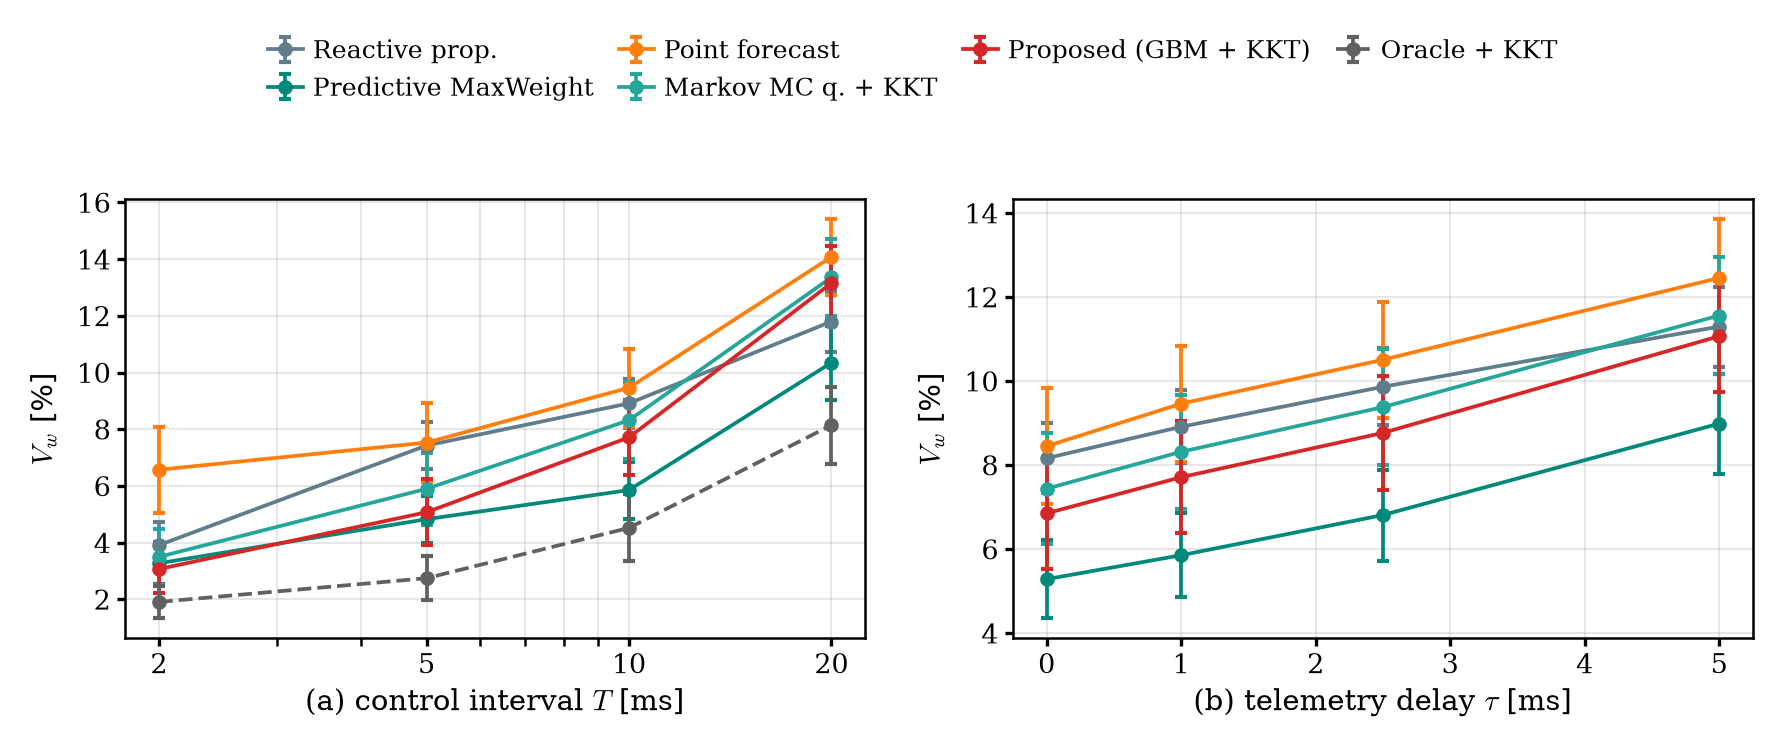
\includegraphics[width=\linewidth]{paper_fig_regime.png}\\
      \small
      \textbf{Operating regime}
      \begin{itemize}\small
        \item $T \le 5$\,ms $\to$ \textbf{reservation} (KKT) wins
        \item $T = 10$--$20$\,ms, short bursts $\to$ \textbf{back-pressure} wins
        \item Long bursts (FTP files, XR frames) $\to$ reservation at every $T$
      \end{itemize}
    \end{column}
  \end{columns}
\end{frame}

% =====================================================================
\section{Part B2: A Bayesian, Decision-Focused Transformer for the Shared Link}
% =====================================================================

\begin{frame}{Starting point: which Transformer, and what we change}
  \scriptsize
  \begin{columns}[T]
    \begin{column}{0.47\textwidth}
      \textbf{Existing architectures we build on}
      \begin{itemize}
        \item \textbf{PatchTST} (Nie et al., ICLR 2023): series cut into patches, one shared encoder per channel.
        \item \textbf{iTransformer} (Liu et al., ICLR 2024): attention \emph{across} variates instead of time.
        \item \textbf{TFT} (Lim et al., 2021): multi-quantile output, static covariates.
        \item \textbf{MC dropout} (Gal \& Ghahramani 2016), \textbf{deep ensembles} (Lakshminarayanan et al.\ 2017).
        \item \textbf{Decision-focused learning} (Donti et al.\ 2017; Elmachtoub \& Grigas 2022).
      \end{itemize}
      \textbf{Closest O-RAN work}: goal-oriented PRB forecasting with TFT (arXiv 2609.17297) trains pinball at a cost-derived level and \emph{avoids} differentiating through the allocation; per cell, no shared link, no deadlines.
    \end{column}
    \begin{column}{0.53\textwidth}
      \textbf{Our modifications (LCQT family)}
      \begin{enumerate}
        \item \textbf{Deadline-aware patch tokens}: each patch carries its own $\rstar$ at the cell's deadline (+ mean, max); a summary token holds the 28 GBM features.
        \item \textbf{Deadline/priority FiLM}: one network for LL and eMBB cells.
        \item \textbf{Link-aware cross-cell layer}: attention over the 8 cells that share the link.
        \item \textbf{Non-crossing quantile head}: $q_k = q_{k-1} + \mathrm{softplus}(a_k)$.
        \item \textbf{Bayesian layer}: ensemble $\times$ MC-dropout posterior, fed to the KKT rule as a \emph{mixture} (keeps epistemic spread).
        \item \textbf{Differentiable KKT layer}: train \emph{through} the coupled capacity constraint (implicit gradient through the shadow price $\lambda^\ast$).
      \end{enumerate}
      \vspace{2pt}
      \textcolor{accent}{We found no paper combining these; each block is prior art.}
    \end{column}
  \end{columns}
\end{frame}

\begin{frame}{LCQT: link-aware cross-cell quantile Transformer}
  \centering
  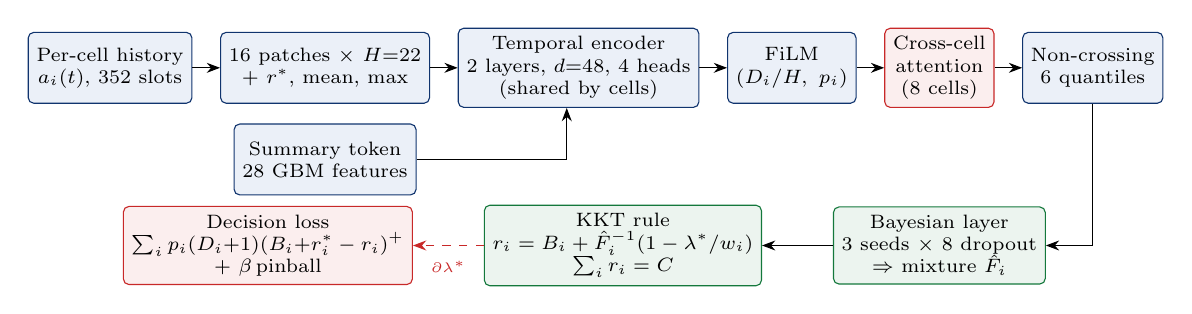
\begin{tikzpicture}[
      font=\scriptsize, >=Stealth,
      box/.style={draw=iitblue, fill=soft, rounded corners=2pt, align=center, minimum height=0.9cm, inner sep=3pt},
      hot/.style={box, draw=accent, fill=accent!8},
      grn/.style={box, draw=good, fill=good!8}]
    \node[box] (hist) {Per-cell history\\$a_i(t)$, 352 slots};
    \node[box, right=0.35cm of hist] (patch) {16 patches $\times$ $H{=}22$\\+ $\rstar$, mean, max};
    \node[box, below=0.25cm of patch] (feat) {Summary token\\28 GBM features};
    \node[box, right=0.35cm of patch] (enc) {Temporal encoder\\2 layers, $d{=}48$, 4 heads\\(shared by cells)};
    \node[box, right=0.35cm of enc] (film) {FiLM\\$(D_i/H,\ p_i)$};
    \node[hot, right=0.35cm of film] (cross) {Cross-cell\\attention\\(8 cells)};
    \node[box, right=0.35cm of cross] (head) {Non-crossing\\6 quantiles};
    \node[grn, below=1.25cm of cross] (bayes) {Bayesian layer\\3 seeds $\times$ 8 dropout\\$\Rightarrow$ mixture $\hat F_i$};
    \node[grn, left=0.9cm of bayes] (kkt) {KKT rule\\$r_i = B_i + \hat F_i^{-1}(1-\lambda^\ast/w_i)$\\$\textstyle\sum_i r_i = C$};
    \node[hot, left=0.9cm of kkt] (loss) {Decision loss\\$\sum_i p_i (D_i{+}1)(B_i{+}\rstar_i - r_i)^+$\\$+\ \beta\,$pinball};
    \draw[->] (hist) -- (patch);
    \draw[->] (patch) -- (enc);
    \draw[->] (feat.east) -| ([xshift=-0.15cm]enc.south);
    \draw[->] (enc) -- (film);
    \draw[->] (film) -- (cross);
    \draw[->] (cross) -- (head);
    \draw[->] (head.south) |- (bayes.east);
    \draw[->] (bayes) -- (kkt);
    \draw[->, dashed, accent] (kkt) -- node[below, font=\tiny, yshift=-2pt]{$\partial\lambda^\ast$} (loss);
  \end{tikzpicture}\\[6pt]
  \footnotesize
  \begin{tabular}{lll}
    \toprule
    Parameters & 63\,k (44\,k without cross-cell layer) & vs.\ $6\times300$ GBM trees \\
    Training & 40 epochs, AdamW + OneCycle, early stop on \textbf{validation} pinball & $\approx$6\,min, 4-core CPU \\
    Data & same train / val / test seeds and target as the GBM & test seeds never seen \\
    \bottomrule
  \end{tabular}
\end{frame}

\begin{frame}{The two non-standard layers}
  \footnotesize
  \begin{columns}[T]
    \begin{column}{0.49\textwidth}
      \begin{block}{Bayesian mixture layer}
        Posterior samples $s = 1..M S$ (members $\times$ dropout passes) give quantile functions $Q_i^{(s)}$. The KKT rule gets the \textbf{mixture}
        \[ \hat F_i(x) = \tfrac{1}{MS}\textstyle\sum_s F_i^{(s)}(x), \]
        not the averaged quantiles. Averaging quantiles throws away the disagreement between samples. With the mixture, a cell whose forecast the posterior is unsure about gets a \textbf{wider} margin at the same $\lambda^\ast$.\\[3pt]
        Dropout seeded per decision slot $\Rightarrow$ runs stay reproducible.
      \end{block}
    \end{column}
    \begin{column}{0.49\textwidth}
      \begin{block}{Differentiable KKT layer}
        Forward: bisection for $\lambda^\ast$ (no gradient). Backward: implicit function theorem on the binding link
        \[ g(\lambda,q) = \textstyle\sum_i r_i(\lambda,q) - C = 0 \;\Rightarrow\; \frac{\partial\lambda^\ast}{\partial q} = -\frac{\partial g/\partial q}{\partial g/\partial \lambda}, \]
        implemented as one Newton step from the detached root. Loss = the pathwise \textbf{shortfall-sandwich} lower bound on dropped bits.\\[3pt]
        Contexts $(B_i, w_i)$ depend on the policy: logged closed-loop on training seeds, then one \textbf{DAgger} round.
      \end{block}
    \end{column}
  \end{columns}
  \vspace{2pt}
  \centering\footnotesize Unit tests: the layer matches the numpy allocator to $10^{-6}$; $\partial\sum_i r_i/\partial q = 0$ when the link is full (budget only moves between cells).
\end{frame}

\begin{frame}{Forecast quality (same validation rows for every model)}
  \scriptsize
  \centering
  \begin{tabular}{lcccccc}
    \toprule
    & \multicolumn{4}{c}{Validation (in distribution)} & \multicolumn{2}{c}{Shift (held out, OOD)} \\
    \cmidrule(lr){2-5}\cmidrule(lr){6-7}
    Model & Pinball & Pinball LL & 90\,\% cov. & 90\,\% width & 90\,\% cov. & LL $q_{0.95}$ cov. \\
    \midrule
    GBM (before) & 0.0224 & 0.0259 & 0.894 & 1.51 & --- & --- \\
    LCQT & \best{0.0214} & \best{0.0251} & 0.902 & \best{1.36} & 0.795 & 0.855 \\
    \quad without cross-cell layer & 0.0213 & 0.0249 & 0.903 & 1.38 & & \\
    \quad unweighted pinball & 0.0213 & 0.0250 & 0.922 & 1.38 & & \\
    LCQT + MC dropout (16) & 0.0214 & 0.0251 & 0.911 & 1.41 & 0.802 & 0.870 \\
    Deep ensemble (3) & \best{0.0212} & \best{0.0248} & 0.912 & 1.37 & 0.806 & 0.864 \\
    \rowcolor{good!10} Ensemble $\times$ MC (3$\times$8) & 0.0213 & 0.0249 & \best{0.919} & 1.40 & \best{0.808} & \best{0.873} \\
    DF-LCQT (decision-focused) & 0.0224 & 0.0273 & 0.907 & 1.38 & 0.830 & 0.822 \\
    \bottomrule
  \end{tabular}
  \normalsize
  \begin{itemize}\footnotesize
    \item The Transformer cuts pinball by \textbf{4.5\,\%} and the 90\,\% interval by \textbf{8\,\%} \emph{at higher coverage} than GBM.
    \item The cross-cell layer and priority weighting do \textbf{not} improve the forecast (ablations equal within noise).
    \item The Bayesian layer moves coverage towards nominal under shift (LL $q_{0.95}$: 0.855 $\to$ 0.873), but cannot remove under-coverage there: the shift is outside training.
    \item DF-LCQT gives up forecast accuracy on purpose: it shades the LL upper tail (LL $q_{0.95}$ coverage 0.88).
  \end{itemize}
  \vspace{-2pt}{\tiny Transformer rows read through the mixture layer (1 sample for LCQT); the direct read-out of LCQT gives 0.909 / 1.38. Ablation rows: direct read-out.}
\end{frame}

\begin{frame}{Closed loop: $V_w$ [\%] on Family S (mean of 20 test seeds)}
  \scriptsize
  \centering
  \begin{tabular}{lccccc}
    \toprule
    Controller & low 0.50 & moderate 0.65 & high 0.80 & flash crowd & shift \\
    \midrule
    GBM + KKT (proposed, before) & 0.15 & 2.15 & 8.00 & 11.76 & 10.04 \\
    LCQT median + water-fill & 0.25 & 3.14 & 9.76 & 13.47 & 11.51 \\
    LCQT + KKT & 0.13 & 2.05 & 7.91 & 11.81 & 10.06 \\
    \quad without cross-cell layer & 0.13 & 2.05 & 7.94 & 11.83 & 10.00 \\
    \quad unweighted pinball & 0.13 & 2.05 & 7.85 & 11.71 & 9.95 \\
    MC-dropout LCQT + KKT & 0.12 & 2.04 & 7.93 & 11.82 & 10.03 \\
    \rowcolor{good!10} \textbf{Bayesian LCQT + KKT} (3$\times$8) & \best{0.12} & \best{2.02} & \best{7.89} & 11.78 & 10.02 \\
    DF-LCQT + KKT & 0.18 & 2.26 & 7.93 & 11.62 & 10.15 \\
    \midrule
    CEM policy (extended study) & 0.13 & 1.77 & 6.57 & 10.20 & 9.73 \\
    Predictive MaxWeight & 0.14 & 1.62 & 6.15 & 9.69 & 10.25 \\
    Oracle + KKT (true $\rstar$) & 0.05 & 0.88 & 4.77 & 8.10 & 5.84 \\
    \bottomrule
  \end{tabular}
  \normalsize
  \vspace{2pt}
  \begin{itemize}\footnotesize
    \item Same traces and seeds for every row; GBM rows re-run and match the stored runs exactly (deterministic simulator).
    \item Best \emph{KKT-rule} variant: \textbf{Bayesian LCQT}. Back-pressure and policy search remain better at moderate--flash load.
  \end{itemize}
\end{frame}

\begin{frame}{Paired per-seed statistics and what carries the gain}
  \begin{columns}[c]
    \begin{column}{0.5\textwidth}
      \centering
      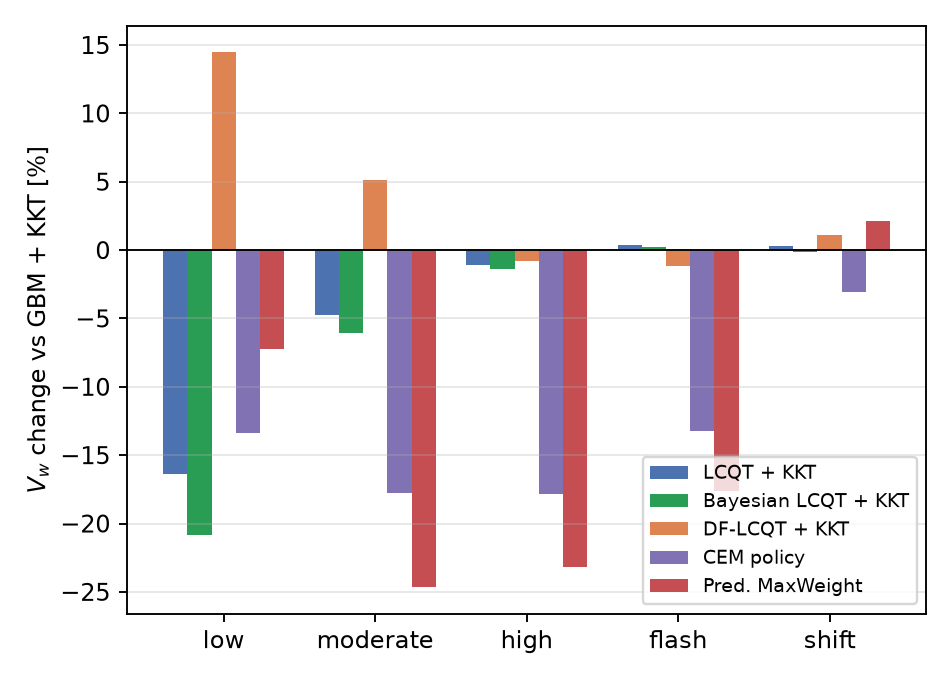
\includegraphics[width=\linewidth]{fig_transformer_delta.png}
    \end{column}
    \begin{column}{0.5\textwidth}
      \scriptsize
      \textbf{Bayesian LCQT vs.\ GBM + KKT} (95\,\% bootstrap CI, wins /20, Holm--Wilcoxon)\\[2pt]
      \begin{tabular}{lcc}
        \toprule
        Scenario & Reduction & Wins \\
        \midrule
        low & \best{$-20.8\%$} [16.0, 28.3] & 20 \\
        moderate & \best{$-6.1\%$} [5.1, 7.0] & 20 \\
        high & \best{$-1.4\%$} [1.0, 1.8] & 20 \\
        flash & $+0.2\%$ (n.s.) & 9 \\
        shift & $-0.2\%$ (n.s.) & 14 \\
        \bottomrule
      \end{tabular}\\[3pt]
      vs.\ plain LCQT: $-0.2$ to $-5.3\%$, all 5 scenarios, $p < 0.03$.
      \begin{itemize}\scriptsize
        \item \textbf{Patch Transformer}: the main gain.
        \item \textbf{Bayesian mixture}: small, consistent extra gain.
        \item \textbf{Cross-cell layer}, \textbf{priority loss}: no gain.
        \item \textbf{DF-LCQT}: $-1.2\%$ in flash ($p<10^{-3}$) but $+14\%$ at low load: the one-horizon surrogate ignores queue carry-over.
      \end{itemize}
    \end{column}
  \end{columns}
\end{frame}

\begin{frame}{Part B2: honest assessment}
  \small
  \begin{columns}[T]
    \begin{column}{0.5\textwidth}
      \begin{exampleblock}{What improved}
        \begin{itemize}\footnotesize
          \item The Bayesian LCQT improves the proposed method on \textbf{every} seed at low--high load and never loses significantly.
          \item The Bayesian mixture layer is the best KKT variant and gives the best calibration under shift.
          \item LCQT is cheaper per decision than GBM (2.7 vs 3.4\,ms).
          \item The differentiable KKT layer works and is unit-tested; validation decision loss $-9\,\%$ after DAgger (each model under its own policy).
        \end{itemize}
      \end{exampleblock}
    \end{column}
    \begin{column}{0.5\textwidth}
      \begin{alertblock}{What did not}
        \begin{itemize}\footnotesize
          \item Gains are small at high load ($-1.4\,\%$). The gap to CEM / predictive MaxWeight (14--28\,\%) is \textbf{structural}, not forecast error. This confirms the extended-study diagnosis.
          \item The decision-focused model's validation gain did not transfer to the test seeds at low/moderate load.
          \item The Bayesian layer costs 17--21\,ms in Python ($>$10\,ms interval): it needs batched / compiled inference on an O-DU.
          \item Synthetic Family S only; G and M not yet run.
        \end{itemize}
      \end{alertblock}
    \end{column}
  \end{columns}
  \vspace{2pt}
  \footnotesize\textbf{Next (done in Part B3)}: keep the forecaster, change the decision structure --- a policy class that contains both strongest baselines.
\end{frame}

% =====================================================================
\section{Part B3: Beating the Strongest Baselines --- Back-Pressure Newsvendor}
% =====================================================================

\begin{frame}{Why the KKT rule loses to back-pressure (S high, 20 test seeds)}
  \centering
  \small
  \begin{tabular}{lcccc}
    \toprule
    Controller (all in \%) & $V_w$ & LL viol. & eMBB viol. & Link util. \\
    \midrule
    KKT rule (GBM) & 8.00 & 3.4 & 12.3 & 72.2 \\
    CEM class-level & 6.57 & 6.0 & 7.1 & 74.7 \\
    Pred.\ MaxWeight (CEM-tuned) & 5.98 & 6.0 & 5.9 & 75.5 \\
    \rowcolor{good!10} \textbf{BPN} (this part) & \best{5.23} & 5.5 & \best{4.9} & \best{76.1} \\
    Oracle + KKT & 4.77 & 0.1 & 9.2 & 74.8 \\
    \bottomrule
  \end{tabular}
  \raggedright
  \begin{itemize}\footnotesize
    \item A budget is a \textbf{per-cell cap}: capacity reserved for a 2-ms cell's upper quantile and not used is \textbf{lost}.
    \item The KKT rule over-protects LL (3.4\,\%) and starves eMBB (12.3\,\%); it uses the link least (72.2\,\%).
    \item Back-pressure fills in queue order with median demands: less waste, but it ignores deadlines and forecast uncertainty.
    \item \textbf{Idea}: fill the base in back-pressure order, \emph{then} spend the leftover on newsvendor margins.
  \end{itemize}
\end{frame}

\begin{frame}{BPN: one policy class that contains both strongest baselines}
  \footnotesize
  \begin{columns}[T]
    \begin{column}{0.55\textwidth}
      \textbf{Stage 1 --- base, back-pressure sharing}\\
      $b_i = a\,Q_i/T + (1-a)\,B_i$ \hfill (drain rate vs.\ deadline backlog)\\
      $d_i = b_i + (1+\mu)\,\hat F_i^{-1}(p^0_{c(i)})$ \hfill (class base level)\\
      Shortage shared $\propto v_{c}\,\big(\pi_i/\bar\pi\big)^{\eta}$, \ $\pi_i = Q_i + \ell H m_i$\\
      ($\eta = 0$: class-weighted water-fill; $\eta = \eta_{\max}$: strict back-pressure order)\\[4pt]
      \textbf{Stage 2 --- leftover by the KKT rule}\\
      $r_i = \max\!\big(r_i^{(1)},\ b_i + \hat F_i^{-1}(1 - \lambda/\omega_{c(i)})\big)$, \ $\textstyle\sum_i r_i = C$\\[4pt]
      \textbf{Contains} (unit-tested, exact under shortage):
      \begin{itemize}
        \item Predictive MaxWeight: $a{=}1,\ p^0{=}0.5,\ \mu{=}$margin, $\eta{=}\eta_{\max}$
        \item CEM class-level policy: $a{=}0,\ p^0{=}$class levels, $v_{\rm LL}{=}w_{\rm LL},\ \eta{=}0$
      \end{itemize}
    \end{column}
    \begin{column}{0.43\textwidth}
      \textbf{Learning $\theta$ (8 parameters)}
      \begin{itemize}
        \item CEM on \textbf{training} seeds only (8 episodes, same as the baselines' search).
        \item Two starts: the tuned optimum of each contained baseline.
        \item Baselines re-tuned with the \textbf{same} search (``CEM-tuned''), so tuning effort is equal.
      \end{itemize}
      \textbf{Learned structure}\\[2pt]
      \scriptsize
      \begin{tabular}{lccc}
        \toprule
        Family & $\eta$ & $a$ & $(p^0_{\rm LL}, p^0_{\rm eMBB})$ \\
        \midrule
        S (bursty) & 6 (greedy) & 0.98 & (0.41, 0.45) \\
        G (3GPP) & 0 & 0.31 & (0.94, 0.73) \\
        M (Markov) & 0 & 0.34 & (0.84, 0.31) \\
        \bottomrule
      \end{tabular}\\[2pt]
      \footnotesize The search \textbf{recovers the regime map}: back-pressure for short bursts, reservation for long ones.
    \end{column}
  \end{columns}
\end{frame}

\begin{frame}{Family S results: $V_w$ [\%] (mean of 20 test seeds)}
  \scriptsize
  \centering
  \begin{tabular}{llccccc}
    \toprule
    Forecaster & Controller & low & moderate & high & flash & shift \\
    \midrule
    \multirow{6}{*}{GBM} & KKT rule (before) & 0.15 & 2.15 & 8.00 & 11.76 & 10.04 \\
    & Pred.\ MaxWeight (grid-tuned) & 0.14 & 1.62 & 6.15 & 9.69 & 10.25 \\
    & Pred.\ MaxWeight (CEM-tuned) & 0.16 & 1.66 & 5.98 & 9.36 & 10.46 \\
    & CEM class-level (re-searched) & 0.13 & 1.73 & 6.58 & 10.23 & 9.76 \\
    & BPN v1 (6 param.) & 0.10 & 1.21 & 5.23 & 8.58 & 9.23 \\
    & \textbf{BPN v2} (8 param.) & 0.10 & 1.21 & 5.32 & 8.70 & 9.26 \\
    \midrule
    \multirow{4}{*}{LCQT} & Pred.\ MaxWeight (CEM-tuned) & 0.15 & 1.59 & 5.82 & 9.17 & 10.38 \\
    & CEM class-level & 0.12 & 1.69 & 6.49 & 10.12 & 9.70 \\
    & BPN v1 & 0.08 & 1.14 & 5.10 & 8.38 & 9.04 \\
    & BPN v2 & 0.08 & 1.16 & 5.25 & 8.59 & 9.24 \\
    \midrule
    \multirow{2}{*}{Bayesian LCQT} & BPN v1 & 0.08 & 1.11 & \best{5.05} & \best{8.34} & \best{8.92} \\
    & \cellcolor{good!10}\textbf{BPN v2} & \cellcolor{good!10}\best{0.07} & \cellcolor{good!10}1.12 & \cellcolor{good!10}5.21 & \cellcolor{good!10}8.55 & \cellcolor{good!10}9.12 \\
    \midrule
    --- & Oracle + KKT (true $\rstar$) & 0.05 & 0.88 & 4.77 & 8.10 & 5.84 \\
    \bottomrule
  \end{tabular}
  \normalsize
  \begin{itemize}\footnotesize
    \item With the \emph{same} forecaster, BPN beats both strongest baselines in every scenario. At high load it is within \textbf{6--10\,\%} of the oracle-informed KKT rule.
    \item The Transformer (B2) now pays off: it helps BPN more than it helped the KKT rule (high: $5.32 \to 5.21$).
  \end{itemize}
\end{frame}

\begin{frame}{Generalisation: Families G (3GPP) and M (Markov) --- $V_w$ [\%]}
  \small
  \centering
  \begin{tabular}{lccccc}
    \toprule
    Controller (GBM forecaster) & G moderate & G high & M moderate & M high & M shift \\
    \midrule
    KKT rule (before) & 5.08 & 8.01 & 0.92 & 4.94 & 5.52 \\
    Pred.\ MaxWeight (CEM-tuned) & 6.75 & 10.02 & 1.61 & 4.82 & 4.82 \\
    CEM class-level (extended study) & 4.58 & 7.17 & 0.88 & 3.93 & 4.17 \\
    CEM class-level (re-searched) & 4.51 & 7.05 & 0.94 & 3.94 & 4.22 \\
    BPN v1 (search from pred.\ MaxWeight) & 5.67 & 8.92 & \best{0.63} & 3.71 & \best{3.72} \\
    \rowcolor{good!10} \textbf{BPN v2} & \best{4.24} & \best{6.81} & 0.68 & \best{3.62} & 3.82 \\
    Oracle + KKT & 3.47 & 6.06 & 0.03 & 1.84 & 2.31 \\
    \bottomrule
  \end{tabular}
  \normalsize
  \vspace{4pt}
  \begin{itemize}\footnotesize
    \item \textbf{BPN v1 lost on G}: its stage 1 is always strict back-pressure, so it cannot represent reservation, which wins on long 3GPP bursts (FTP files). Its training cost was also worse (0.070 vs 0.055).
    \item \textbf{v2 fixes it} by containing the reservation policy. Training cost (BPN v2 / best baseline): S 0.0387 / 0.0436, G 0.0527 / 0.0555, M 0.0196 / 0.0226.
  \end{itemize}
\end{frame}

\begin{frame}{BPN v2 vs.\ the best baseline in each scenario}
  \begin{columns}[c]
    \begin{column}{0.55\textwidth}
      \centering
      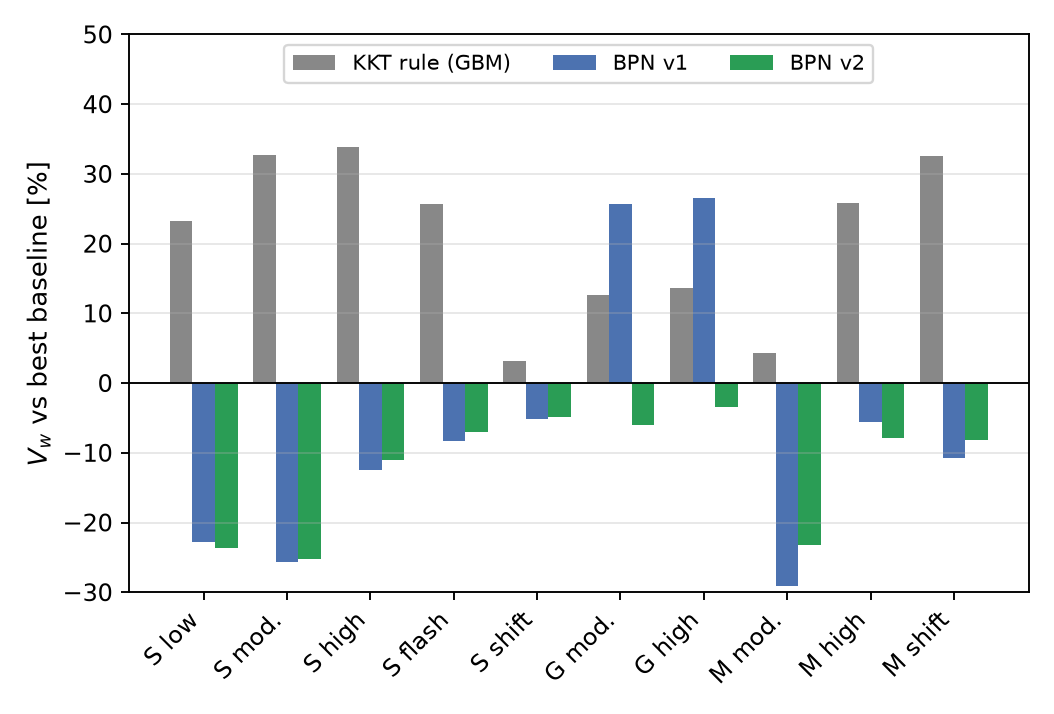
\includegraphics[width=\linewidth]{fig_bpn_vs_best.png}
    \end{column}
    \begin{column}{0.45\textwidth}
      \scriptsize
      \textbf{Paired, 20 test seeds} (Holm--Wilcoxon)\\[2pt]
      \begin{tabular}{lcc}
        \toprule
        Scenario & vs.\ best baseline & Wins \\
        \midrule
        S low & $-23.7\%$ & 15 \\
        S moderate & $-25.3\%$ & 20 \\
        S high & $-11.0\%$ & 20 \\
        S flash & $-7.0\%$ & 20 \\
        S shift & $-4.8\%$ & 20 \\
        G moderate & $-5.9\%$ & 20 \\
        G high & $-3.4\%$ & 19 \\
        M moderate & $-23.3\%$ & 20 \\
        M high & $-7.9\%$ & 20 \\
        M shift & $-8.2\%$ & 20 \\
        \bottomrule
      \end{tabular}\\[3pt]
      \textbf{10/10 scenarios, 3 families}, all $p \le 0.024$.\\
      ``Best baseline'' = the better of pred.\ MaxWeight and CEM class-level, each in its best tuning.
    \end{column}
  \end{columns}
\end{frame}

\begin{frame}{Part B3: what it means for publication}
  \small
  \begin{columns}[T]
    \begin{column}{0.5\textwidth}
      \begin{exampleblock}{What is now claimable}
        \begin{itemize}\footnotesize
          \item A controller that \textbf{beats both strongest baselines}, each in its best tuning, in all 10 scenarios of 3 families, on paired tests.
          \item \textbf{Equal search effort}, training seeds only; the baselines are special cases of the policy class.
          \item The learned exponent \textbf{explains} when to reserve and when to back-pressure: an interpretable result, not a black box.
          \item Fast: 2.2--3.5\,ms per decision (Python), inside the 10\,ms interval (the Bayesian forecaster is not: 20\,ms).
        \end{itemize}
      \end{exampleblock}
    \end{column}
    \begin{column}{0.5\textwidth}
      \begin{alertblock}{Still needed for a top venue}
        \begin{itemize}\footnotesize
          \item \textbf{Real traces} (measured per-cell PRB / fronthaul).
          \item \textbf{More baselines}: a deep-RL xApp (PPO) with the same observation; Lyapunov drift-plus-penalty with deadline queues.
          \item Sensitivity to $T$, $\tau$ and load for BPN (only $T = 20$, $\tau = 2$ so far).
          \item The policy is learned per family; transfer between families is not yet tested.
          \item No optimality proof for the hybrid; the KKT optimality holds only for stage 2.
        \end{itemize}
      \end{alertblock}
    \end{column}
  \end{columns}
\end{frame}

% =====================================================================
\section{Conclusions and Future Work}
% =====================================================================

\begin{frame}{What we do \emph{not} claim}
  \footnotesize
  \begin{itemize}
    \item \textbf{No real-world validation}: three simulated families. Family G uses standard 3GPP models but our own round-robin scheduler and single-link fronthaul.
    \item \textbf{Part A} compression figures are from the earlier run (the \texttt{src/} package is not in the repository); the inversion benchmark uses random well-conditioned matrices, not channel matrices.
    \item \textbf{Kernels}: 10--15$\times$ is vs.\ single-threaded numpy+LAPACK (2.5--4$\times$ per thread); no MKL/Eigen comparison; on CPU the Newton tracker loses to a tuned exact inverse; RMT-WS components are largely prior art.
    \item \textbf{No closed-loop optimality or stability claim}: propositions cover feasibility, equal weighted risk, backlog-first and a linear miscalibration bound.
    \item \textbf{No universal superiority}: only $-4$\,\% vs.\ proportional under flash crowds; loses at $T = 20$\,ms, at $\ge 0.86$ load, near-tie at $\tau = 5$\,ms; ML adds $\approx 2$\,\% under shift.
    \item \textbf{Priority trade}: the claim holds for LL weight $\ge$ 2--3.
    \item In the extended comparison, CEM policy search and predictive MaxWeight beat the KKT rule in 9/10 scenarios; only the BPN hybrid (B3) beats them, and it is learned per family at $T = 20$, $\tau = 2$ only.
    \item \textbf{Transformer (B2)}: Family S only; gains at high load are small ($-1.4\,\%$); the Bayesian layer is too slow in Python for a 10\,ms interval; decision-focused training did not transfer. ``No prior paper'' means none found in our search, not a proof.
  \end{itemize}
\end{frame}

\begin{frame}{Conclusions}
  \footnotesize
  \begin{block}{Part A}
    Structure-aware encoders: \textbf{13--16$\times$} at $\approx -20$\,dB (BFP $\sim 4\times$), \textbf{3--6$\times$ faster} than SVD. A learned \emph{iteration} works where a direct neural inverse fails. A \textbf{fused C/AVX-512 RZF kernel} runs the whole precoder 10--15$\times$ faster than numpy+LAPACK, fitting $K \le 16$ in a 0.5\,ms slot; RU-side precoding cuts fronthaul by $\approx 72\,\%$.
  \end{block}
  \begin{block}{Part B}
    Forecasting the \textbf{deadline-feasible rate} as a \textbf{range} and splitting the link with a closed-form \textbf{KKT rule} is the best of 12 controllers in all scenarios of two families: \textbf{$-11$ to $-43$\,\%} vs.\ the forecast median, \textbf{$-19$ to $-70$\,\%} vs.\ deadline-aware reactive, every seed, $p < 0.01$. \textbf{B3}: the \textbf{back-pressure newsvendor} beats the strongest baselines in \textbf{10/10} scenarios of 3 families ($-3$ to $-25$\,\%).
  \end{block}
  \begin{columns}[T]
    \begin{column}{0.5\textwidth}
  \begin{block}{Extended study}
    $\rstar$ linked to effective bandwidth (bounds valid, loose). Learned class levels and predictive back-pressure go further: the gap is \textbf{structural} (B2 confirms it).
  \end{block}
    \end{column}
    \begin{column}{0.48\textwidth}
  \begin{exampleblock}{Take-away}
    Compression sets the load regime; allocation matters most between $\approx$0.5 and 0.8 load. Keep the structure, learn only what is uncertain.
  \end{exampleblock}
    \end{column}
  \end{columns}
\end{frame}

\begin{frame}{Future work}
  \footnotesize
  \begin{columns}[T]
    \begin{column}{0.5\textwidth}
      \textbf{Part A}
      \begin{itemize}
        \item Restore the \texttt{src/} package and regenerate Exp.\ 1--4
        \item Benchmark on realistic channel matrices
        \item SIMD / GPU real-time encode path ($<100\,\mu$s)
        \item ACAFS as a near-RT RIC xApp (E2SM)
        \item Kernels: compare vs MKL batched / Eigen; AMX; GPU/NPU for the Newton path; cache-blocking for $K > 32$
        \item Benchmark vs ChebI-NS, Chebyshev-RZF, TPE
      \end{itemize}
      \textbf{A + B}
      \begin{itemize}
        \item Make the compression width a \textbf{per-cell knob} of the allocation rule (trade signal quality for load)
      \end{itemize}
    \end{column}
    \begin{column}{0.5\textwidth}
      \textbf{Part B}
      \begin{itemize}
        \item Validation on measured per-cell PRB traces
        \item Controller that \textbf{switches} between reservation and back-pressure from estimated burst length vs.\ interval
        \item Coupled calibration (adjust $\lambda$, or calibrate on unconstrained error)
        \item Skill-weighted mix of learned and window quantiles as fallback
        \item Switch-level queue model; compiled implementation for an O-DU
        \item Stronger policy search (neural policy, more episodes)
        \item B3: real traces; PPO xApp baseline; BPN over $T$, $\tau$; cross-family transfer
      \end{itemize}
    \end{column}
  \end{columns}
\end{frame}

\begin{frame}[fragile]{Deliverables and reproducibility}
  \footnotesize
  \begin{columns}[T]
    \begin{column}{0.5\textwidth}
      \textbf{Repository}
      \scriptsize
      \begin{itemize}
        \item \texttt{matinv\_bench/} --- inversion benchmark, InverseNets
        \item \texttt{cmatinv/}, \texttt{experiments\_v2/} --- complex inversion, RMT-WS, 38.901 channels, Exp.\ 5--18
        \item \texttt{kernels/} --- fused C/AVX-512/OpenMP precoder
        \item \texttt{experiments/} --- Part A Exp.\ 1--4, extended pipeline
        \item \texttt{fhlm/} --- simulator, traffic (S, G, M), forecasters, 19 controllers, theory, figures, tables
        \item \texttt{fhlm/transformer.py}, \texttt{decision\_focused.py}, \texttt{hybrid.py} --- Parts B2, B3
        \item \texttt{tests/} --- 16 + 14 + 8 + 4 + 4 tests (capacity every slot, no future leakage, bound validity, KKT-layer gradients, \dots)
        \item \texttt{results/} --- all CSVs / logs / figures
      \end{itemize}
      \textbf{Papers}
      NCC 2027 submission (6 pp.); 11-page extended manuscript.
    \end{column}
    \begin{column}{0.5\textwidth}
      \textbf{Reproduce}
      \scriptsize
\begin{verbatim}
python -m pytest tests -q
python -m fhlm.train
python -m fhlm.run_experiments tune
python -m fhlm.run_experiments main
python -m fhlm.make_figures
python -m fhlm.train_transformer
python -m fhlm.decision_focused
python -m fhlm.run_transformer_study
python -m fhlm.hybrid cem --policy bpn2
bash experiments/run_extended.sh
sh kernels/build.sh
python experiments_v2/run_all.py
\end{verbatim}
      \normalsize
      \small Every number in the papers is a macro generated from the CSVs.
    \end{column}
  \end{columns}
\end{frame}

\begin{frame}{Key references}
  \scriptsize
  \begin{itemize}
    \item O-RAN WG4, \emph{Control, User and Synchronization Plane Specification} (split 7-2x, BFP compression).
    \item 3GPP TR 38.801, TR 38.901, TS 38.214, TR 36.814, TR 38.838.
    \item L.\,M.\,P.\ Larsen, A.\ Checko, H.\,L.\ Christiansen, ``A survey of the functional splits proposed for 5G mobile crosshaul networks,'' \emph{IEEE COMST}, 2019.
    \item G.\,O.\ P\'erez, J.\,A.\ Hern\'andez, D.\ Larrabeiti, ``Fronthaul network modeling and dimensioning meeting ultra-low latency requirements for 5G,'' \emph{JOCN}, 2018.
    \item L.\ Wang, S.\ Zhou, ``On the fronthaul statistical multiplexing gain,'' \emph{IEEE Commun.\ Lett.}, 2017.
    \item S.\ Lag\'en et al., ``Fronthaul compression control for shared fronthaul access networks,'' \emph{IEEE Commun.\ Mag.}, 2022.
    \item D.\ Bega et al., ``DeepCog'' (2019) and ``AZTEC'' (2020): forecast-driven capacity allocation.
    \item I.\ Gibbs, E.\ Cand\`es, ``Adaptive conformal inference under distribution shift,'' NeurIPS 2021.
    \item N.\ Halko, P.\,G.\ Martinsson, J.\,A.\ Tropp, ``Finding structure with randomness,'' \emph{SIAM Review}, 2011.
    \item J.-Y.\ Le Boudec, P.\ Thiran, \emph{Network Calculus}, Springer, 2001.
    \item M.\,J.\ Neely, \emph{Stochastic Network Optimization}, 2010;\ L.\ Huang et al., predictive back-pressure, 2016.
    \item G.\ Hadley, T.\,M.\ Whitin, \emph{Analysis of Inventory Systems} (multi-item newsvendor), 1963.
    \item W.\ Willinger et al., self-similar ON/OFF traffic, \emph{IEEE/ACM ToN}, 1997.
    \item D.\ Anick, D.\ Mitra, M.\,M.\ Sondhi, Markov fluid sources, \emph{BSTJ}, 1982.
    \item Y.\ Nie et al., PatchTST, ICLR 2023;\ Y.\ Liu et al., iTransformer, ICLR 2024;\ B.\ Lim et al., Temporal Fusion Transformer, \emph{IJF} 2021.
    \item Y.\ Gal, Z.\ Ghahramani, MC dropout, ICML 2016;\ B.\ Lakshminarayanan et al., deep ensembles, NeurIPS 2017.
    \item P.\ Donti, B.\ Amos, J.\,Z.\ Kolter, task-based end-to-end learning, NeurIPS 2017;\ A.\ Elmachtoub, P.\ Grigas, ``Smart predict-then-optimize,'' \emph{Mgmt.\ Sci.} 2022.
  \end{itemize}
\end{frame}

\begin{frame}[noframenumbering]
  \centering
  \vspace{2em}
  {\Huge\textcolor{iitblue}{\textbf{Thank you}}}\\[1.5em]
  {\Large Questions?}\\[2em]
  \small Mayank Yadav \quad\textbullet\quad Harshvardhan Choudhary
\end{frame}

% =====================================================================
\appendix
\section*{Backup}
% =====================================================================

\begin{frame}[noframenumbering]{Backup: what is new here?}
  None of the ingredients is new on its own (quantile GBM, constrained newsvendor / KKT, water-filling, conformal inference, network-calculus service curves). The candidate contribution is the \textbf{combination and its fair evaluation} in the shared-fronthaul setting:
  \begin{enumerate}
    \item Forecasting the \textbf{deadline-feasible rate} $\rstar$, not the traffic volume.
    \item A rule that turns the forecast \textbf{range} into budgets under the shared-link constraint by cutting every cell at the same weighted risk --- margins \emph{derived}, not tuned.
    \item An evaluation that is fair by construction and reports where the method does \textbf{not} win.
  \end{enumerate}
  \vspace{0.5em}
  \textbf{Closest work}: Lag\'en et al.\ 2022 (shared 7-2x link, reactive compression, no forecast); Bega et al.\ DeepCog/AZTEC (single predicted number, no per-cell deadlines); Cohen et al.\ 2023 (conformal for one URLLC stream; our ablation shows per-stream correction does not carry over).
\end{frame}

\begin{frame}[noframenumbering]{Backup: likely questions}
  \small
  \begin{description}[Why synthetic traffic?]
    \item[Leakage?] Train 1000--1015, val 2000--2003, test 3000--3019; forecaster frozen before test; features use past slots only (tested); normalisation by config constants.
    \item[Why GBM, not LSTM?] Six quantile models train in 12\,s, well calibrated, CPU-only; the ablation shows the model is not where most of the gain is.
    \item[Why synthetic traffic?] No public per-cell PRB-level fronthaul traces (ColO-RAN is $\ge$250\,ms); hence Family G built from 3GPP models.
    \item[Why are violations high?] Heavy-tailed bursts at 0.8 load with budgets held 10\,ms; even the oracle loses 13\,\% of eMBB bits. Paired differences are the result.
    \item[Is the allocation optimal?] Only for the one-interval surrogate (separable concave, KKT = global optimum). No closed-loop claim.
    \item[Why does ACI hurt?] LL misses in a coupled split are partly caused by the shortage split, not forecast bias; offsets over-reserve LL.
    \item[Could the DU export its schedule?] Yes where an interface exists (e.g.\ CTI); our setting is budgets committed before the schedule is known.
  \end{description}
\end{frame}

\begin{frame}[noframenumbering]{Backup: trade-off and paired reductions}
  \begin{columns}[c]
    \begin{column}{0.5\textwidth}
      \centering
      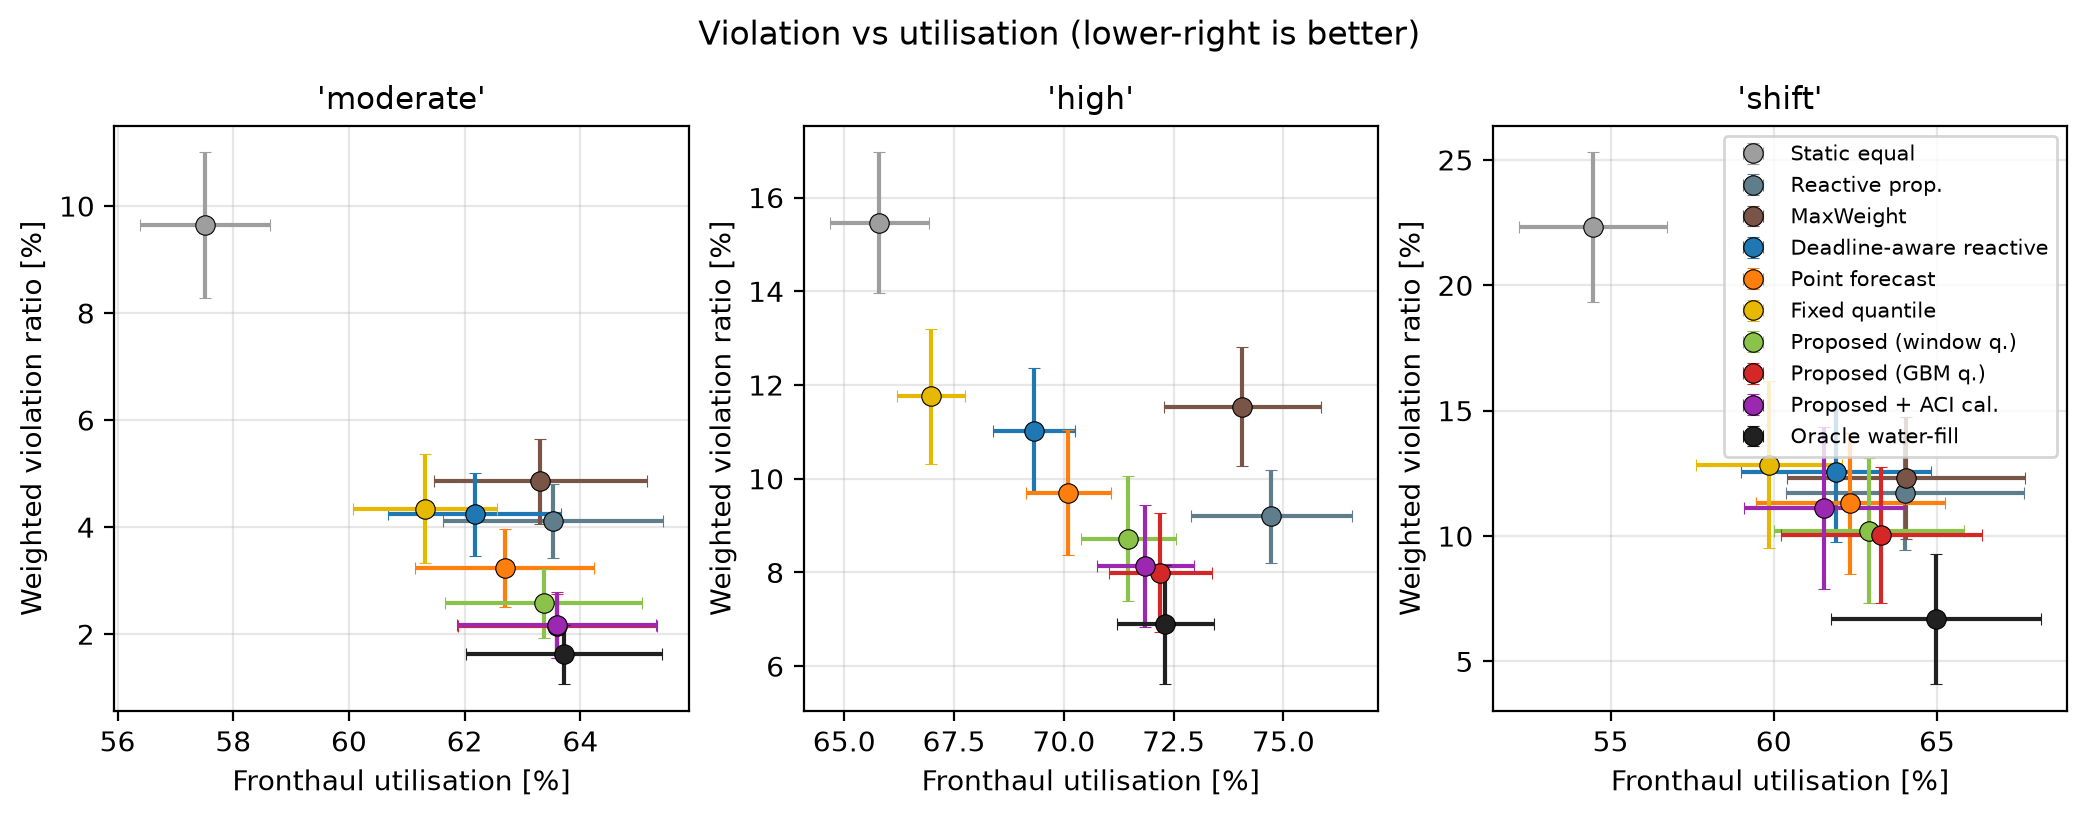
\includegraphics[width=\linewidth]{fig3_tradeoff.png}
    \end{column}
    \begin{column}{0.5\textwidth}
      \centering
      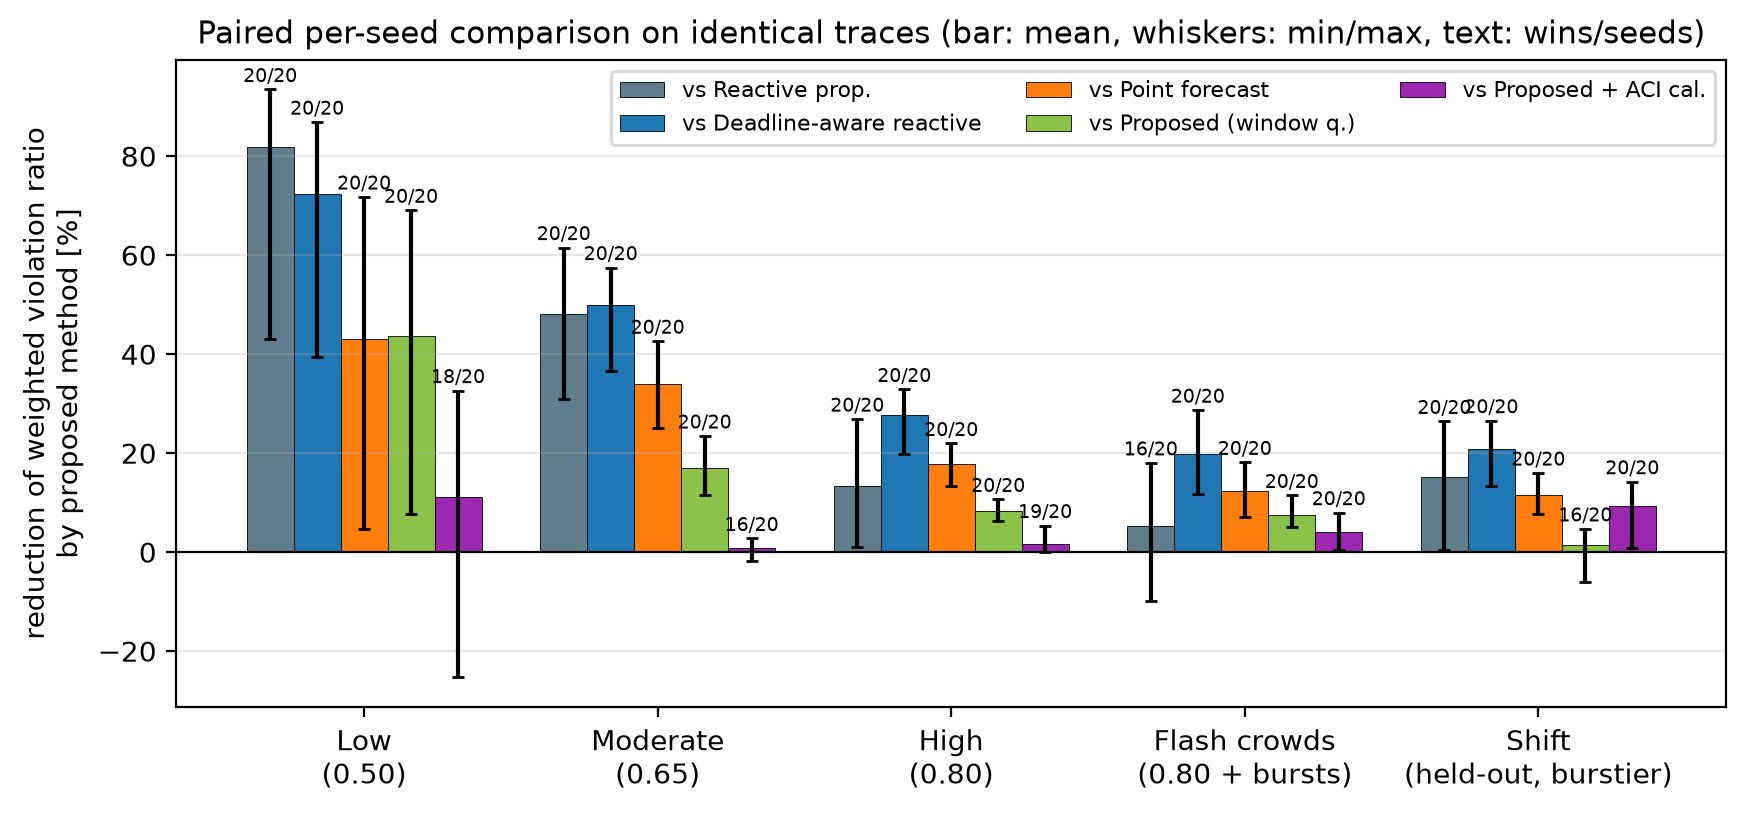
\includegraphics[width=\linewidth]{fig8_paired_reduction.png}
    \end{column}
  \end{columns}
\end{frame}

\begin{frame}[noframenumbering]{Backup: Family G figure and telemetry delay}
  \begin{columns}[c]
    \begin{column}{0.5\textwidth}
      \centering
      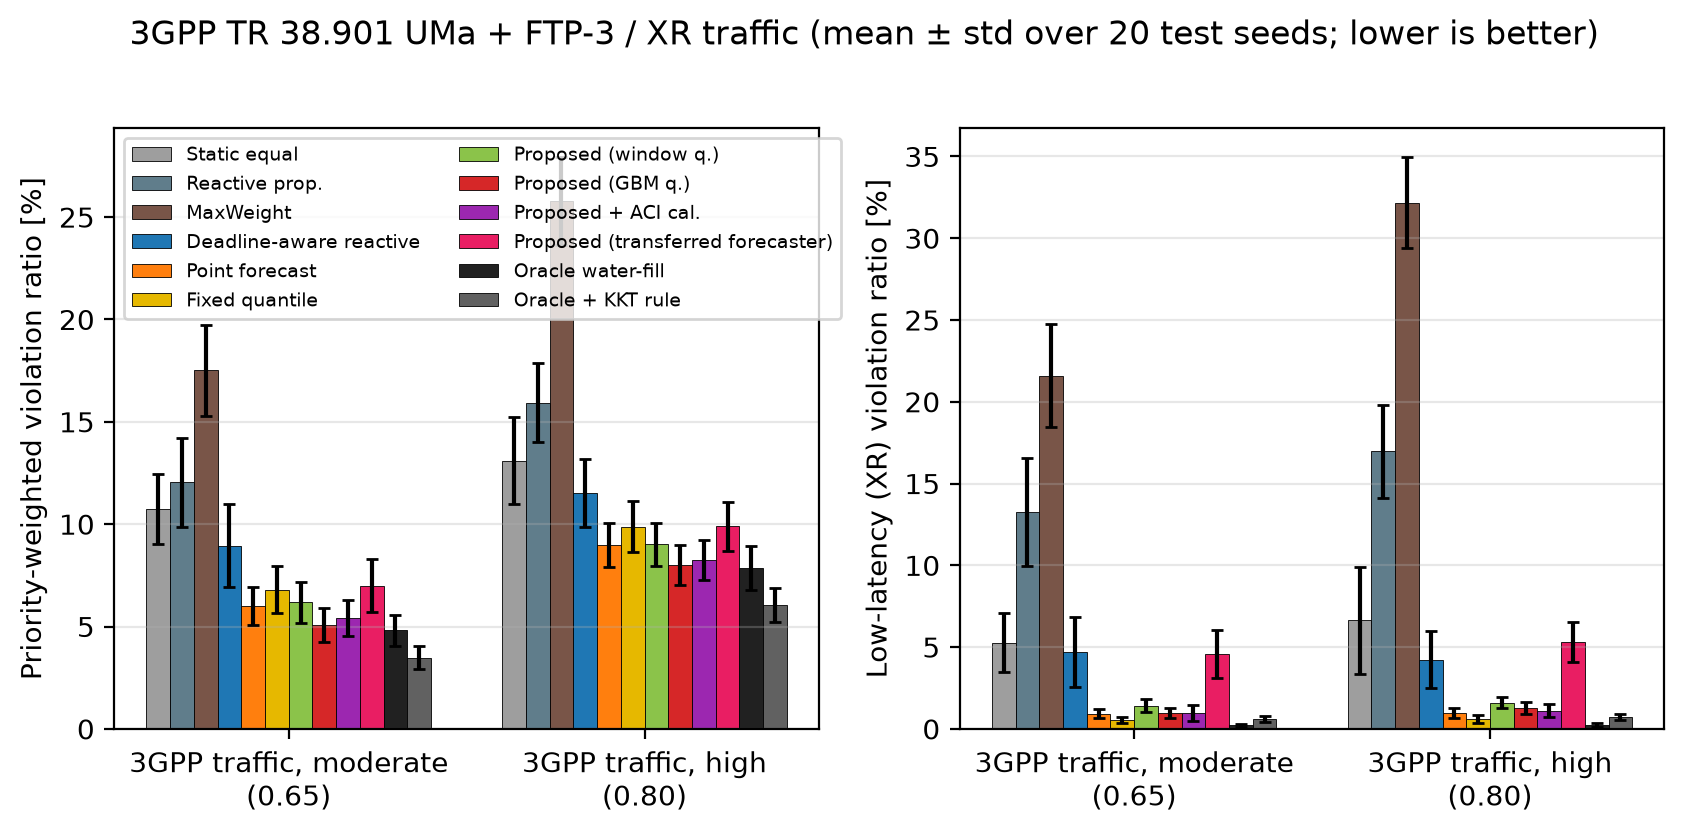
\includegraphics[width=\linewidth]{fig12_tgpp.png}
    \end{column}
    \begin{column}{0.5\textwidth}
      \centering
      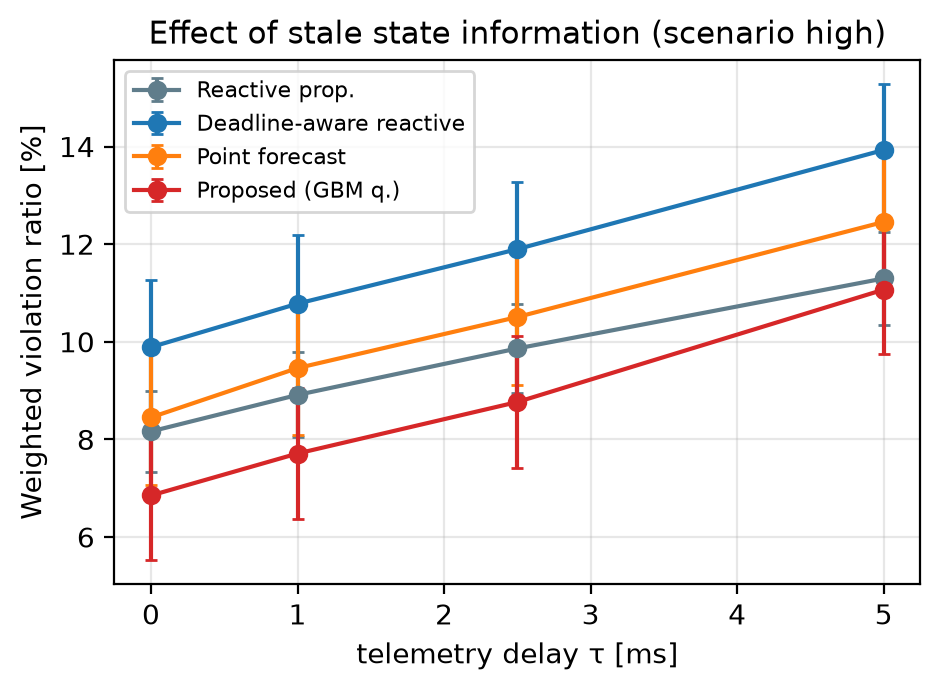
\includegraphics[width=\linewidth]{fig11_delay.png}
    \end{column}
  \end{columns}
\end{frame}

\end{document}
